\documentclass{cmspaper}
\usepackage{graphicx}
\usepackage{amssymb}
\usepackage{amsmath}
%\usepackage{draft}
\usepackage{lineno}
\usepackage[table]{xcolor}
\usepackage{url}

\linenumbers % For draft version

%----------------------------------------
% On ins�re ici les diff�rentes parties du rapport 
%----------------------------------------

\begin{document}

\begin{titlepage}
%\internalnote{IN-2013/XXX}
%\cmsnote{2007/000}
\date{\today}
\date{Draft proposal for discussions v 2.3}
\title{Development of CMS L1 Tracking Trigger Vertical Slice System Demonstration}
\begin{Authlist}
Ted Liu*, Sergo Jindariani, Nhan Tran, Lindsey Gray, Jim Hoff, Jamieson Olsen \\
Fermilab\\
Kristian Hahn*, Kevin Sung, Marco Trovato, Stanislava Sevova \\
Northwestern University\\
Ivan Furic*, Souvik Das, Michele de Gruttola, Jacobo Konigsberg\\
University of Florida\\
\end{Authlist}

\Anotfoot{*}{Denotes PI/Contact person for the corresponding institution}
%\Anotfoot{b}{INFN, Pisa, Italy}
%\Anotfoot{c}{Fermilab, USA}

\begin{abstract}
CMS plans to pursue rich physics program in the HL-LHC era. In order to fulfill these agressive goals in the environment of very high pile-up envisioned for HL-LHC, CMS must preserve its ability to identify in real time signatures of events originating from interesting physics processes. Use of tracker information in L1 provides highly efficient handle for the pile-up mitigation and will be in focus of the CMS Phase 2 upgrades. In this proposal we request funding for the R\&D program aimed at developing a tracking trigger solution for the CMS upgrade. This R\&D program will allow US to provide key contributions and lead the construction of a Vertical Slice Demonstration System, which will comprise a full tracking trigger path and will be used with simulated high-luminosity data to measure trigger latency and efficiency, to study overall system performance and to identify appropriate solutions to possible bottlenecks. Funding is requested to support engineering efforts to develop critical components of the system: the ATCA board used for data transfer/formatting, the associative memory (AM) chip for pattern recognition, and the AM chip carrying mezzanine. Funding to develop corresponding software and firmware is also included. 
\end{abstract}
\end{titlepage}
\newpage
\tableofcontents
\newpage

%
% Uncomment the part you are interested in 
%

%\section{R\&D Overview}

%\begin{center}
%{\Large\bf Introduction}
%\end{center}

%\vspace{0.5cm}

\subsection{Physics Motivations}

As outlined recently by the US P5 report as well as by the European Strategy reports and CERN management, the high luminosity LHC (HL-LHC) is one of the top priorities for the particle physics community. The CMS collaboration intends to pursue a rich physics program in the era of the HL-LHC. Precision measurements of the properties of the newly discovered Higgs boson will clearly be central to the CMS physics program.  The relatively low transverse momentum of Higgs decay products will make Higgs identification a formidable task in the harsh collision environment of the HL-LHC.

Virtual corrections to the Higgs mass imply that its natural value should be very far from the electroweak scale. In the absence of fine-tuning, the low value observed for the Higgs mass strongly suggests the presence of new physics. A variety of new physics scenarios (composite Higgs, extra dimensions and super-symmetry, for example) naturally tame radiative Higgs mass corrections. It is therefore essential for CMS to have the ability to cover a large region of phase space for potential new particle production. This phase space, like the Higgs, is near the threshold of current CMS triggering capabilities. With the existing L1 system, the higher trigger rates anticipated in the HL-LHC will necessitate significantly higher trigger thresholds, drastically diminishing the discovery potential of CMS.

Perhaps the largest open question the HL-LHC can address involves the production of dark matter. Physics analyses at the LHC are capable of confirming or denying the existence of dark matter in regions of space that direct and indirect detection experiments can not reach. Signatures of dark matter in a proton collision environment typically involve missing transverse energy (MET), a quantity that is difficult to utilize in high pileup conditions.  Recently, however, novel MET reconstruction techniques have demonstrated an encouraging degree of pileup insensitivity.  These techniques rely heavily on tracking information, and can in principle be utilized for MET calculations performed in the trigger, as well as in the offline environment.

The physics program outlined above involves signatures with relatively low energy or with poorly resolved final state objects. Such objects require low L1 trigger thresholds that are robust against the high intensity and pileup conditions expected at the HL-LHC. The trigger thresholds used in current physics analyses cannot be maintained at the HL-LHC without incorporating tracking information into the earliest stage of the event selection process. Maintaining low trigger thresholds in order to preserve high efficiency for low-pt objects is the primary physics motivation of the work proposed here.



\subsection{R\&D Overview}


\noindent 

While the discovery of the Higgs boson is a major achievement, many questions remain, including those regarding the precise mechanism of electroweak symmetry breaking and the nature of dark matter. In order to maximize the potential for discovery, CMS must preserve or improve its ability to identify, in real time, events with signatures consistent with the Higgs boson and new particle decays. This is a highly non-trivial task given the high pile-up conditions anticipated in the HL-LHC era.

At CMS, the only major detector not used in the present L1 trigger is the Silicon Tracker. It has become clear that the development of a L1 tracking trigger will be required for CMS to maintain physics acceptances for basic objects (leptons, photons, jets and MET) in the HL-LHC era. Without L1 tracking, the resolution of quantities traditionally used in L1 will seriously degrade due to pileup effects.  Trigger thresholds would need to increase in response, which would lead to unacceptable losses in trigger efficiency.  Most of the anticipated CMS physics program would slip out of reach.

Consequently, the design of the Phase-II CMS Tracker must allow for an effective implementation of the tracking trigger.  Because the construction of the Phase-II Tracker will take many years, its design must be finalized soon (by the 2017 TDR).  A silicon-based L1 tracking trigger has never been realized at this scale and thus it is imperative that its feasibility be demonstrated before the design of the Phase-II Tracker can be finalized.  Silicon-based Level-2 tracking trigger systems based on associative memory were successfully implemented in the past~\cite{bib:Rist-89}~\cite{bib:Ade-07} and are being actively explored at present~\cite{bib:FTK-TDR}. Experience with these systems will serve as useful input to the design of the CMS L1 tracking trigger. However the higher occupancies anticipated at the HL-LHC and the low latencies required at L1 (about serveral $\mu$s for the track finding stage) present us with a formidable set of challenges that must be attacked with a well organized R\&D project. The participation of CMS institutions with strong expertise in modern high-speed electronics and pattern recognition technologies will be crucial for the success of this important R\&D program. 

%The short time available for the design and implementation of the L1 tracking trigger demonstration system %poses additional challenges as it does not allow sufficient time for starting R\&D efforts from scratch. 
A number of USCMS institutions led by Fermilab have established a strong generic R\&D program in the area of silicon-based tracking trigger. This R\&D program, funded mostly by non-CMS sources until last year, has so far yielded excellent prototype results and put USCMS in the unique position to develop a working solution for the CMS L1 track trigger. The long-term goal of this R\&D effort is to develop these critical technologies to the point where we can ultimately propose them as a viable solution to the problems of HL-LHC L1 track triggering. Given the fact that Tracker Upgrade TDR is due in a few years,
the progress made so far by this R\&D has well positioned us to take the next important step to establish a Vertical Slice Demonstration System. We have proposed a new architecture and system demonstration design~\cite{bib:CMS_TT_Demo} to the CMS Phase-II Tracker community, and this has been well-received. This system will comprise a full tracking trigger path and will be used with simulated high-luminosity data to measure trigger latency and efficiency, to study overall system performance and to identify appropriate solutions to possible bottlenecks. The proposed system is not intended to be final; rather, serves the purpose of an existence proof. If a functional vertical slice can be demonstrated with today's technology, Moore's law and developments in the semiconductor industry guarantee that the tracking trigger will become less expensive and more performant as we progress toward the HL-LHC.

	Processing each beam crossing implies finding and fitting thousands of tracks starting from a collection of "stubs" (hit pairs) from the front-end Tracker sensors. 40M beam crossings per second must be processed  with a maximum latency of order of a few microseconds. The total raw computation power needed to solve this problem is huge, several orders of magnitude larger than what has ever been used for L1 triggering in the past. The problem obviously calls for massive parallelism. We choose a processing scheme in which data from different bunch crossings or from different regions of the detector in the same crossing are processed in parallel.  For the purpose of regional multiplexing, we divide the detector into 48 angular regions (6 in $\eta$ times 8 in $\phi$) we call "towers". We assign multiple processing engines to each tower so that data from that  tower and from different crossings may be processed in parallel. 
In such a parallel system, one signficant problem is how to optimally distribute data among the various processors. Data from the same crossing, coming from different detector elements, must be assembled and delivered to the same processing unit for track reconstruction. Data from different crossings, coming from the same detector element, must be delivered to different processing units for optimal time multiplexing. The subdivision of the detector into geographical towers, does not lead to an exact corresponding subdivision of the track parameter space. Data coming from a given geographical tower may need to be delivered to multiple parameter space regions. This happens, in particular, when a stub comes from a detector element close to the border between geographical towers, due to the finite curvature of charged particles in the magnetic field and finite size of the luminous region along the beam axis. 

	In addition to the complex data dispatching challenge, there is the obvious challenge of finding and fitting hundreds of billions of tracks every second. This requires extremely fast pattern recognition algorithms. The Associative Memory~\cite{bib:Rist-89} uses a massively parallel architecture to tackle the intrinsically complex combinatorics of track finding algorithms, avoiding the typical power law dependance of execution time on occupancy and solving the pattern recognition in times roughly proportional to the number of hits. This is of crucial importance given the large occupancy fluctuations typical of hadronic collisions. 
The design of an Associative Memory system capable of dealing with the complexity of HL-LHC collisions and with the short latency required by Level 1 triggering poses significant, as yet unsolved, technical challenges.
For this reason, an aggressive R\&D program at Fermilab has been lanuched to advance the state of-the-art in associative memory technology  (3D VIPRAM~\cite{bib:VIP-11} R\&D is funded by DOE CDRD program~\cite{bib:VIP-12}).

Because the Associative Memory approach is thus far the only proven solution to hardware-based tracking triggers in a hadron collider environment (albeit only for Level 2 triggers applications), it is chosen as the baseline for the demonstration in what follows.  The overall system architecture we are proposing, however, is open and flexible, and could be used to support a variety of pattern recognition engines.  This will provide for testing and direct comparisons with possible alternative pattern recognition scheme, such as the tracklet-based approach, described in a separate proposal.


%Although silicon-based tracking trigger at Level-2 trigger has been implemented successfully using the %associative memory approach, the speed of such an approach needs to be demonstrated before it can %become a viable solution for CMS L1 tracking trigger.  such as the tracklet based approach orginally %developed for the Long Barrel detector concept. The tracklet approach for Barrel-Endcap detector geometry %is now being pursued by the Cornell group.

%Overall architecture
	For the reasons above, the design of the overall architecture is focused on the need for efficient dispatching of the data for time and regional multiplexing, and on providing a common, flexible framework for pattern recognition and track fitting. Efficient data dispatch for time and regional multiplexing requires high bandwidth, low latency, and flexible real time communication between processing nodes.  A completely interconnected, ``full mesh'' backplane is a natural fit to these criteria. A custom full mesh enabled ATCA board called Pulsar II has been designed at Fermilab with the goal of creating a scalable architecture abundant in flexible, non-blocking, high bandwidth board-to-board communication channels. The Pulsar II hardware will be the workhorse for the vertical slice demonstration. The architecture we are proposing for the CMS L1 tracking trigger demonstration permits high bandwidth inter-board communication. 
The full-mesh backplane is used to time-multiplex the high volume of incoming data in such a way that I/O demands are manageable at the board and chip level. The resulting architecture will provide an early technical demonstration using existing technology, will allow for the exploration and comparison of various approaches for pattern recognition and track fitting.

% Given that Advanced Mezzanine Card (AMC) specifications are designed to work with both ATCA and %microTCA, the architecture naturally allows for the long-term integration of Tracker DAQ (AMC based) and %tracking trigger activities. 

%\noindent The purpose of this R\&D proposal is to build a vertical slice demonstration test bench to 
%demonstrate track finding and to identify possible bottlenecks and find solutions, using technology that is %available today. This "Vertical Slice" will process simulated data with HL-LHC occupancy at full speed, to %allow us to study and improve the system and tracking performance (such as latency, efficiency and fake %rate). 
%Based on past experience, we believe that the final technology choices for the final implementation of L1 %track finding can be delayed until about four years from the start of commissioning. The goal of this R\&D is %to demonstrate that the track finding can be done so that the tracker detector design can be finalized in the %near future. 

The proposed system architecture is described in the following section. We describe an affordable demonstration system that can be designed and built within 2-3 years.  We then define the ”Vertical Slice” that we propose as the deliverable of this R\&D project. Next, we describe the track finding approach we are pursuing, and discuss the advantages and challenges related to this approach.  We then discuss the work that has been accompished thus far and that which is required in the coming two years.  We close with the funding request. This USCMS R\&D project, if adequtely funded, will allow our community to focus attention on the complex challenges of L1 tracking, to compare different possible solutions to the fundamental pattern recognition and track fitting problems in the HL-LHC era, and to gain the experience necessary to design the final system.


%Main components

%Fiber data transmission,
%ATCA crates,
%Full mesh backplane,
%Fiber receivers,
%Pattern Recognition Boards,
%Pattern Recognition Mezzanines,
%AM as a possible incarnation (3d technology),
%Inter-tower communication,

%Bandwidth and latency considerations



\section{Technical Description and Deliverables}

\subsection{Introduction}


\noindent 

For CMS at HL-LHC, the bandwidth required to bring all data from the massive outer silicon detector reaches 100 Tbps.  Every 25 ns, all tracks with $p_{T}$ above $2\rm~GeV/c$ from (on average) 140 interactions need to be fully reconstructed.
Current estimates show that only a few microseconds will be available for L1 trigger processing.  This includes the time needed for data dispatch to the trigger towers, pattern recognition, track fitting.  Because each of these processes must be accomplished within a very short time, communication between processing elements in different towers requires very high bandwidth and very low latency. Extremely fast and effective track fitting is also required.  This is as high performance as computing gets.  L1 tracking for the HL-LHC will require the most advanced real time processing technology.



%As mentioned earlier, the CDF SVT-style Associative Memory chip (we will call it PRAM, Pattern Recognition Associative %Memory, to emphasis its purpose for HEP) is a departure beyond conventional CAMs. Like conventional CAMs, PRAMs store %address patterns and look for matches between incoming hits and those addresses for a given detector layer. At this level, the %match is expected to be either exact (Binary CAM) or partial (Ternary CAM) and an array of Match Flags is the typical output. A %PRAM has an array of Match Flag Latches which capture and hold the results of the match until reset for the next event. As the %hits from the various layers of the detector for the same event arrive, the PRAM is looking for matches from one candidate %address to one or more stored address patterns. The PRAM organizes stored address patterns into roads, which are linked %arrays of several stored address patterns from different detector layers. Each stored address in a road is from a different layer %in the detector system. These linked addresses represent a path that a particle might traverse through the layers of the %detector (hence the name "road"). The ultimate goal of the PRAM is to match real particle trajectories to those roads. Like a %conventional CAM, a PRAM flags a match when a candidate address matches a stored pattern address for a given detector %layer. However, before the PRAM does anything with that match, it must find matches in all (or majority of) the elements %(layers) that constitute a road. It should be emphasized that compared to commercially available CAMs, such as Network %Search Engine, the PRAM has the unique ability to search for correlations among input words received on different clock cycles. 
%This is essential for tracking trigger applications since the input words are the detector hits arriving from different layers at %different times. They arrive at the chip without any specific timing correlation. Each pattern has to store each fired layer until %the pattern is matched or the event is fully processed. Even in the case of a level-1 trigger application, which is largely %synchronous, this feature will still be important. One unique feature of this approach is that the pattern recognition of the %event is done as soon as the last hit arrives, which makes the approach a promising candidate for L1 track trigger. However, %the requirements for L1 track trigger application will be very different from that for L2, and the system interface of the chip has %to be fully redesigned and the performance has to be optimized.

In the traditional SVT-like AM approach, pattern recognition is solved by the Associative Memory, while track fitting is done in FPGAs using a linear approximation of the dependence of the track parameters on the exact location of the hits within each road. Because roads are narrow, this linear approximation works very well and the track fitting stage is much simplified and fast~\cite{bib:Ann-09} using pre-calculated track parameters for hits in the center of the road, and applying corrections that are linear in the exact position of the hits in each layer. Although roads are narrow, there is still a finite probability (especially with high occupancy at HL-LHC) that multiple hits may fall within the same road for a given detector layer, requiring multiple fits with different hit combinations and leading to longer execution times. To reduce latency, the occurrence of multiple hits from the same detector layer in the same road must minimized.  Consequently, roads must be made as narrow as possible, which requires higher number of patterns that must be stored in the AM. This is why an aggressive R\&D program focused on achieving higher AM densities is an important component of the effort needed to reach the unprecedented low latencies required for silicon based tracking at the HL-LHC.

The PRAM pattern density can be improved by optimizing the design in single-layer chips (2D), using custom cell designs with smaller feature size technology. An R\&D effort on-going at INFN aims to use 65 nm technology to improve AM design for the ATLAS FTK application (a L2 tracking trigger).  INFN now has in hand a 65 nm AM prototype, the AMchip05.  A predecessor, the INFN AM06, is expected to be submitted in Spring 2015. The AMchip05 or AM06 have not been designed or optimized for L1 track trigger applications; however, if availble, these chips could be used for the initial testing of the CMS L1 tracking trigger demonstration system.

\noindent The on-going R\&D effort at Fermilab explores the use of both conventional 2D and emerging 3D technology in the design of a future generation of PRAM chip (based on the VIPRAM~\cite{bib:VIP-11},~\cite{bib:VIP-12} approach) specifically for the needs of the L1 CMS tracking trigger. The Fermilab VIPRAM R\&D project has two goals.  The first is to increase in pattern density through the use of vertical integration and circuit and geometrical (layout) enhancements. This project will continue through FY15 for proof-of-principle of the 3D VIPRAM concept and is funded by DOE CDRD. The second is to increase speed and to improve the system interface, specifically with regard to Level 1 Tracking Trigger applications for CMS at HL-LHC.


%\noindent The architecture we propose is based on ATCA with a full-mesh backplane. The large inter-board communication %bandwidth provided by the full-mesh backplane is used to time multiplex the high volume of incoming data in such a way that %the I/O bandwidth demands are manageable at the board and chip level, making it possible for an early technical %demonstration with existing technology. The resulting architecture is scalable, flexible and open. For example, it allows %different pattern recognition architectures and algorithms to be explored and compared within the same platform. 

%For these reasons, although the system we propose is designed to allow the experimentation of different solutions to fast track %finding and fitting, we consider the Associative Memory approach as the baseline against which other new methods will be %compared. However, the design of an Associative Memory system capable of dealing with the much higher complexity of the %HL-LHC collisions, with an input event rate several orders of magnitude larger than ever done before, and with the much %shorter latency required by Level 1 triggering, poses significant, still unsolved, technical challenges. In fact, the entire system %design as well as board and chip level design will be very different for L1 tracking trigger comparing with that of L2 tracking %trigger applications.  An aggressive R\&D program is needed and is currently ongoing at Fermilab, based on quite a few years %of generic R\&D effort already done.

\noindent Establishing international collaborations within CMS to work on this project is essential. 
For most recent status of tracking trigger activities within CMS, please see presentations at the recent joint meeting of front-end, TK-DAQ and Track Finding meeting~\cite{bib:joint-meeting}, a summary of L1 track trigger progress report is also available~\cite{bib:summary}. Both INFN/Italy and Lyon/France have joined us to work on the vertical slice demonstration using associative memory approach, while others are interested in contributing or exploring possible new track finding algorithms on the same hardware platform. For example, INFN Italy has been working together with the Atlas FTK team exploring the possibility of using FTK associative memory chips for the CMS L1 tracking trigger demonstration. INFN is working closely with Fermilab to develop the pattern recognition mezzanine for the Pulsar II board to host the FTK AMchips (note that another mezzanine is being designed specifically for the associative memory chips being developed at Fermilab).  Experience gained with the FTK AMchips will be useful for guiding the design of a dedicated, CMS L1 associative memory chip at Fermilab. 

Beisdes the hardware development, one of the main activities in the coming year in USCMS (FY2015) will consist of extensive simulation efforts done by physicists, in order to to establish technical specifications based on Phase 2 physics goals. Due to the intrinsic massive parallel processing hardware nature of the AM operation, there is a clear challenge in using software based simulation to emulate the hardware performance. The development of simulation tools for the Associative Memory approach in CMS has been so far lead by the Lyon group, with significant progress made recently towards making the machinery work. The AM Simulation Camp~\cite{bib:AM-CAMP} at CERN in July 2014 has attracted many people and groups to attend, and many from USCMS. However, much of the work still remain to be done. Fermilab/LPC/USCMS have been working and will be more involved in the simulation efforts in FY2015.






\subsection{Track Trigger System Architecture}


\subsubsection{Tracker geometry and Trigger Towers }

\noindent 

Multiple challenges must be faced at the different stages of the processing chain.  First, data needs to be transferred out of the Tracker at the necessary speed.  Stubs from thousands of silicon modules must then be formatted, organized into $\eta-\phi$ trigger towers, duplicated and shared across tower boundaries as needed.  Next, pattern recognition and track fitting must be performed.  Finally, all reconstructed  tracks must be processed to form an intelligent trigger decision. A coherent system design for a Level-1 track trigger must consider each of these aspects.

For simplicity, we assume that the FEDs are upstream, receive fibers from the modules, and pass the relevant stub data to the track trigger system.  One could further consider an architecture in which the FED resides in the same ATCA shelf as the track trigger processing boards; however, the focus of this document is the Vertical Slice Demonstration System, not DAQ readout, so do not attempt to specify FED details here.
The FED interface will need to be defined for demonstration purposes, however the actual FEDs do not need to be involved in the tracking trigger demonstration.


\noindent The found stubs are sent from the modules using a block synchronous data transfer scheme which tolerates random occupancy fluctuations while bonding latency. The current plan is to have the data from 8 consecutive beam crossings as one block. The front-end designers are finalizing the baseline of the data formats after much work investigating different format variants for robustness against rate fluctuations, ease of implementation, impact on power consumption, etc. While choosing the 8 crossings scheme as our current working assumption, our strategy is to design the downstream components to be flexible enough to handle different possible formats. 


\begin{figure}[ht!]
\centering
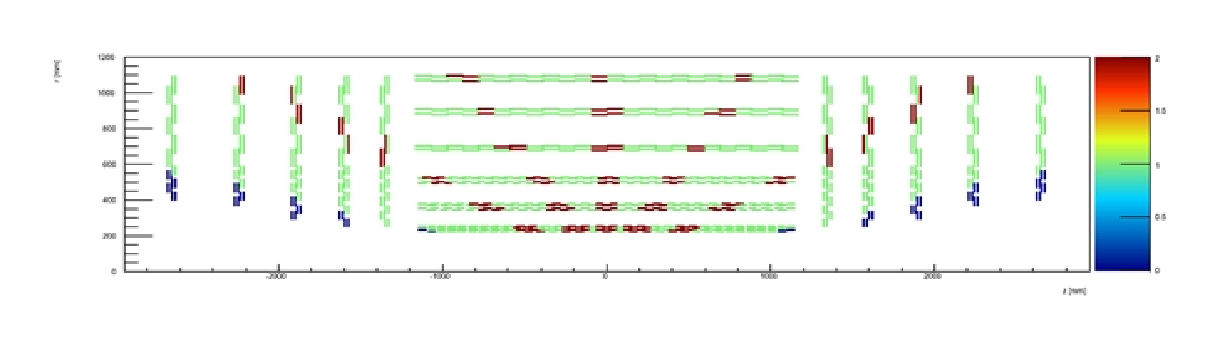
\includegraphics[width=0.75\columnwidth]{Plots/SecDef_RZ.eps}
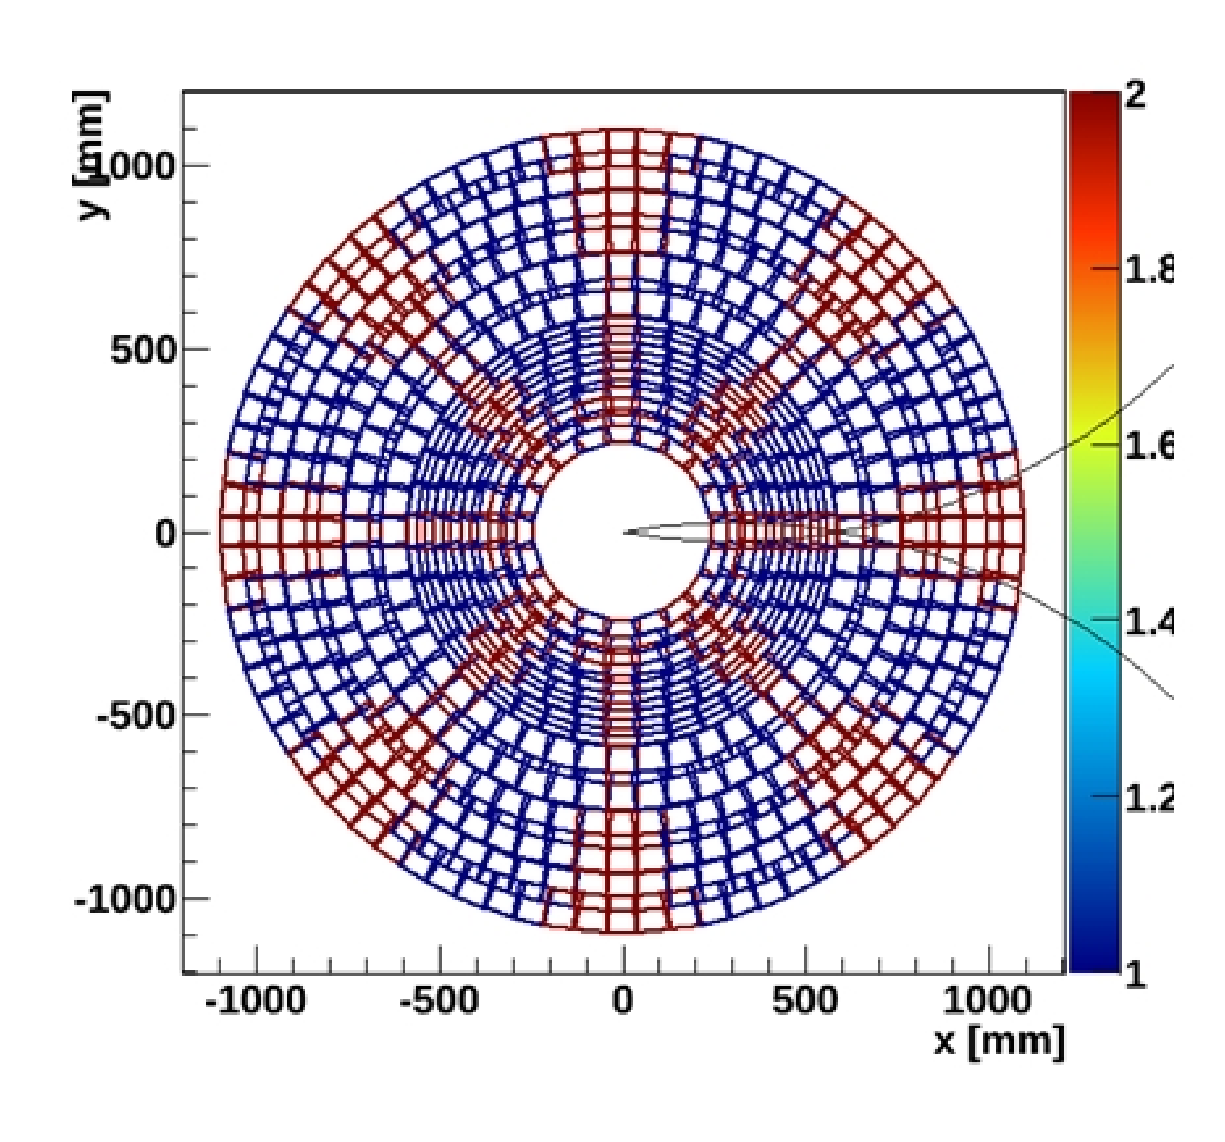
\includegraphics[width=0.2\columnwidth]{Plots/SecDef_XY.eps}
\caption{Six sectors in $\eta$ (left). Note that the symmetry around $\eta=0$ will provide for easier cable grouping. Eight sectors in phi (right).}
\label{fig:SecDef_RZ}
\end{figure}

\noindent 
Stubs from the 15K silicon modules must be delivered to the correct trigger towers.  Detailed data sharing studies have been performed for the Barrel-Endcap (BE) Tracker geometry with different trigger tower partitions.  Based on these studies, a 6 (in $\eta$) x 8 (in $\phi$) = 48 trigger tower partition has been chosen as the baseline configuration (see Figures~\ref{fig:SecDef_RZ}). Detailed studies have been performed on data sharing assuming the default 48 tower partition with a minimum $p_T$ of 2 GeV and track origin smearing in $z\pm 7$ cm. Figure~\ref{fig:TT_config} shows the number of trigger towers that stubs from a given module must be delivered to under these conditions. When a stub is in the middle of the trigger tower, it will have to be delivered to only one tower (to the native trigger tower). When a stub is near the boundary in phi or eta (but not both), it will have to be delivered to two towers. If a stub is at both the boundaries in eta and phi, it will have to be delivered to four towers. Note that four towers is the maximum number of towers any stub must be delivered to. 


\noindent The subdivision of the tracker into 48 trigger towers is shown in Figure~\ref{fig:TT_config} top, where the colored lines indicate all needed interconnections among the trigger towers. 
A unique feature of this arrangement is that any given trigger tower needs only to be connected with its immediate eight neighbors for stub sharing.  Studies have shown that this feature is essentially independent from the minimum pT threshold and track origin smearing in z. 

\begin{figure}[ht!]
\centering
%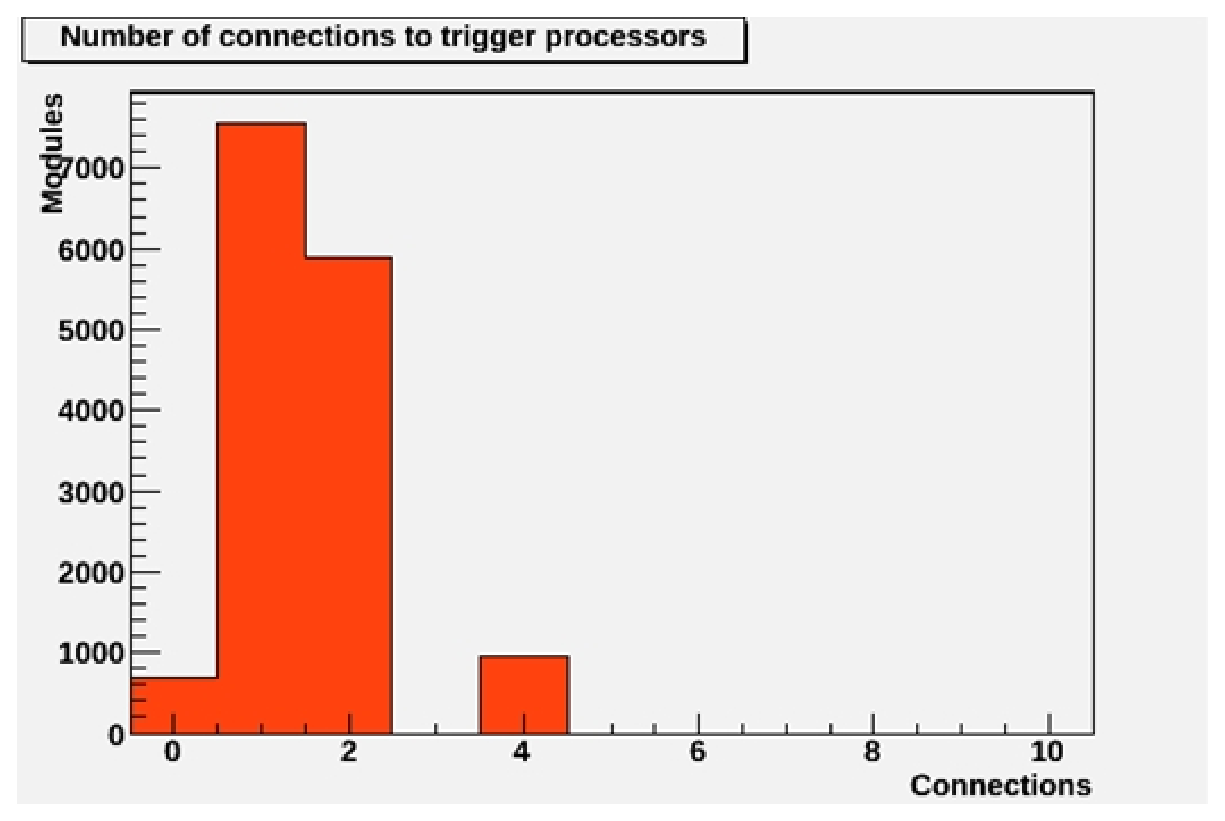
\includegraphics[width=0.45\columnwidth]{Plots/SecDef_N.eps}
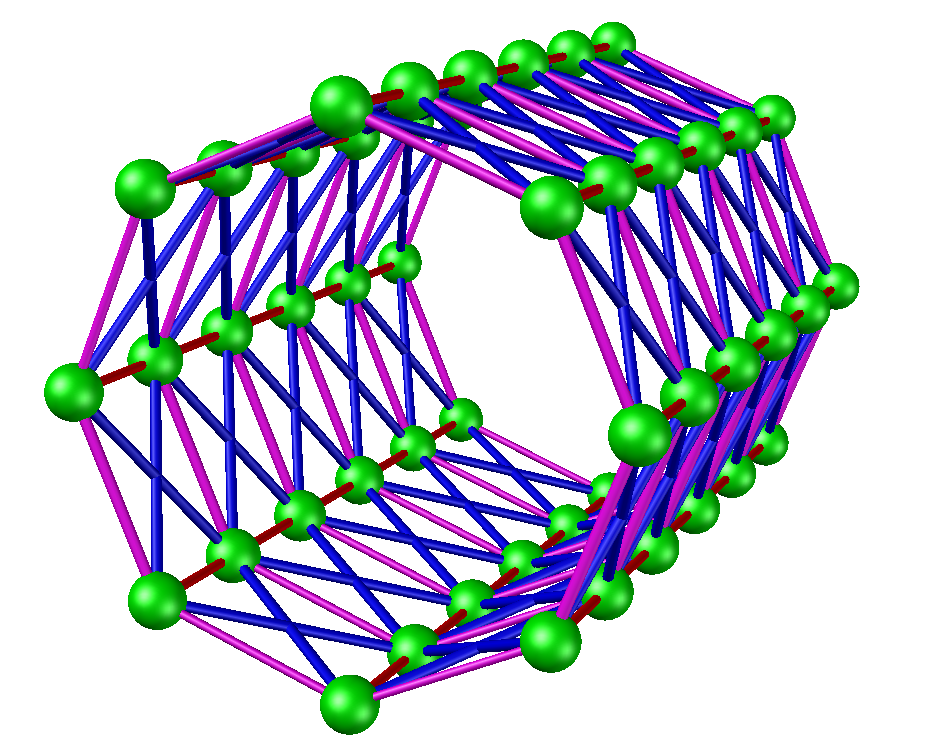
\includegraphics[width=0.4\columnwidth]{Plots/CMS_L1_48_towers.png}
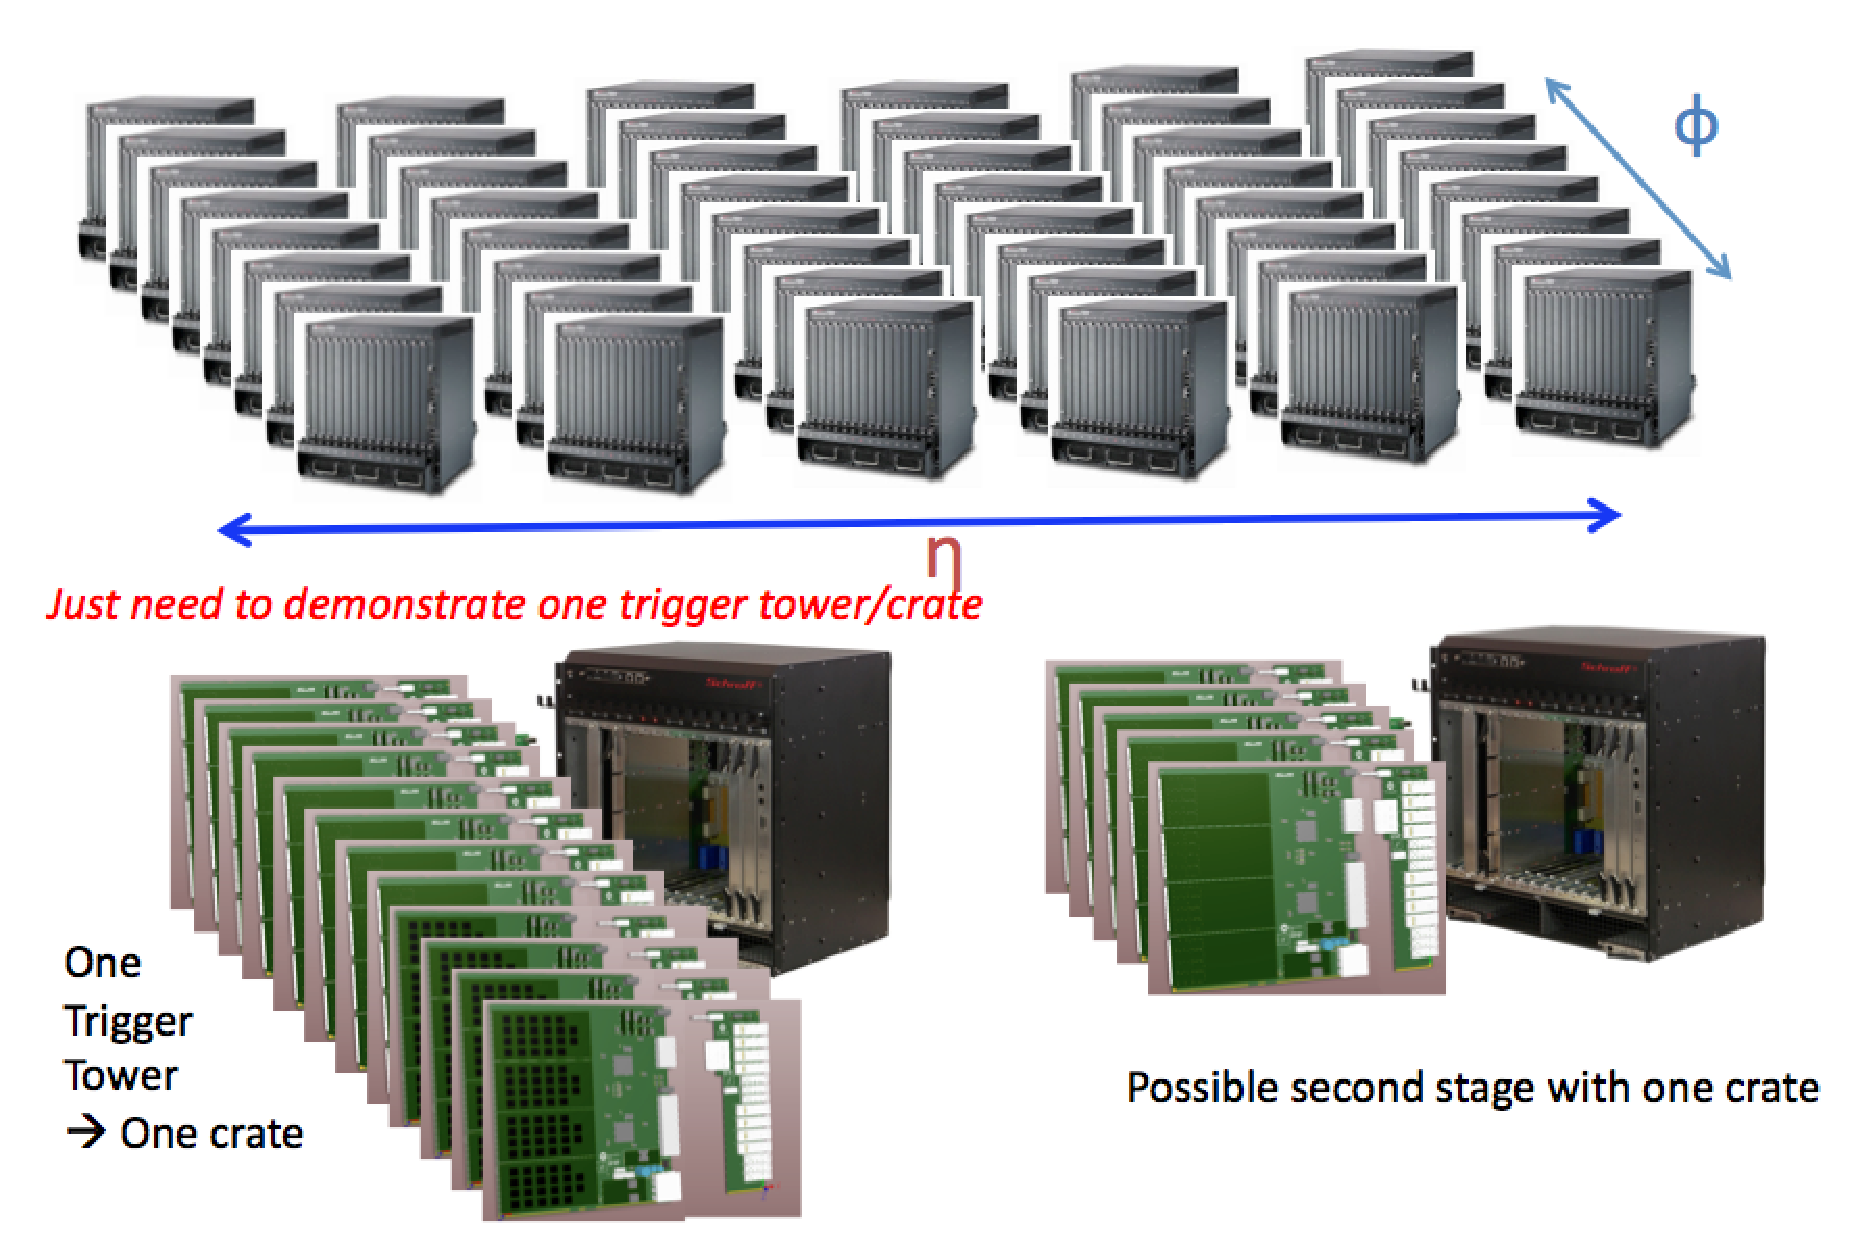
\includegraphics[width=0.7\columnwidth]{Plots/System_1.eps}
\caption{
Top: Conceptual view of the proposed CMS phase II L1 tracking trigger towers.  The formation is organized as 48 trigger towers (6 $\eta$ x 8 $\phi$).  Each node in this diagram represents a trigger tower processor engine.  Within each crate the full mesh backplane is used for time multiplexing of the incoming data, while the data sharing between towers is handled with inter-crate fiber links.
Bottom: 
A simple system configuration that can be built with today's technology assumes one 
ATCA shelf per trigger tower (the actual system will likely be smaller in the future).
}
\label{fig:TT_config}
\end{figure}

\subsubsection{System Architecture}

\noindent The tower processor platform must support large number of fiber transceivers, which are used for receiving input links and sharing data between neighboring towers.  A flexible, high bandwidth backplane is also required to quickly transfer data between boards.  The boards should be large enough to support pattern recognition engines and fiber connections. Given these requirements, we propose a full mesh 14 slot ATCA shelf to support the tower processors. An ATCA shelf is typically an air-cooled 13U rack mounted chassis consisting of 14 slots.  The first two slots are reserved for Ethernet switch blades.  Switch blades may include a fast CPU and are often used for controls and other system functions.  The remaining 12 slots are used for processor or payload blades.  In a full mesh ATCA backplane each pair of slots is directly connected with a multi-lane bidirectional serial channel capable of supporting sustained 40 Gbps data transfers.  A modern "40G" full mesh ATCA shelf has a total aggregate bandwidth of over 7 Tbps, not including external I/O.

\noindent 

For simplicity, we assume one ATCA shelf per trigger tower for the moment. Following this assumption, if the L1 Tracking Trigger system were built today, the full system would comprise 48 ATCA shevles, as shown in  Figs.~\ref{fig:TT_config}. Our assumption is, of course, very conservative.  The actual system will most likely be significantly smaller due to rapid progress in technology developement.
Note that connections between tower processor shelves are limited to eight nearest neighbors, and this can be easily achieved. 

In additon, as shown in Figure~\ref{fig:TT_config}, an additional shelf could act as a second stage processor.  Each board in this shelf could receive tracks from complete events, allowing track duplication removal to be implemented at this stage.  With more boards to sharing data over the full mesh backplane, it is also possible to implement jet related triggers, vertexing capabilities, track based MET calculations, etc.

%\begin{figure}[ht!]
%\centering
%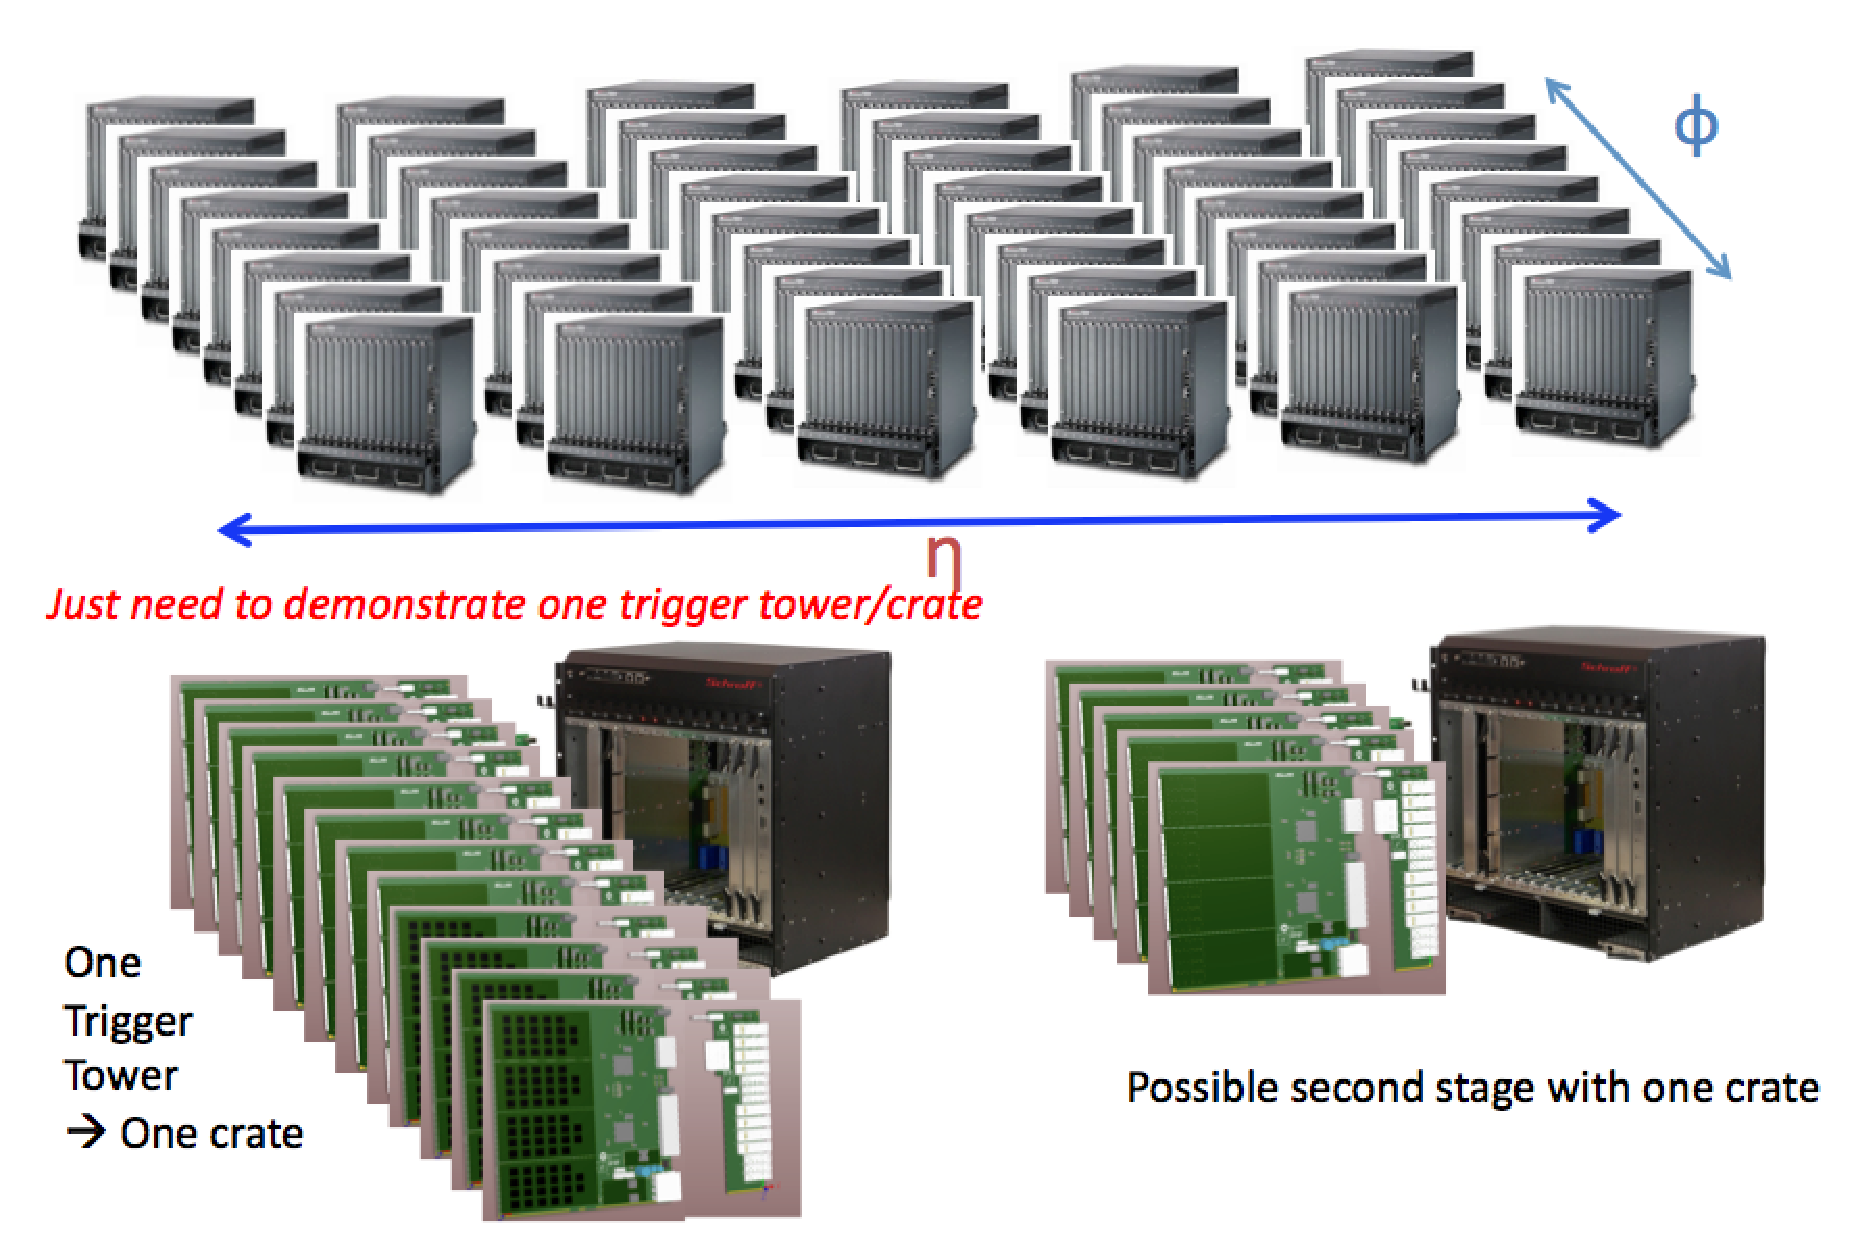
\includegraphics[width=0.7\columnwidth]{Plots/System_1.eps}
%\caption{Possible system configuration with today's technology by simply assuming one ATCA shelf per %trigger tower (the actual system will likely be smaller in the future)}
%\label{fig:System_1}
%\end{figure}

%\begin{figure}[ht!]
%\centering
%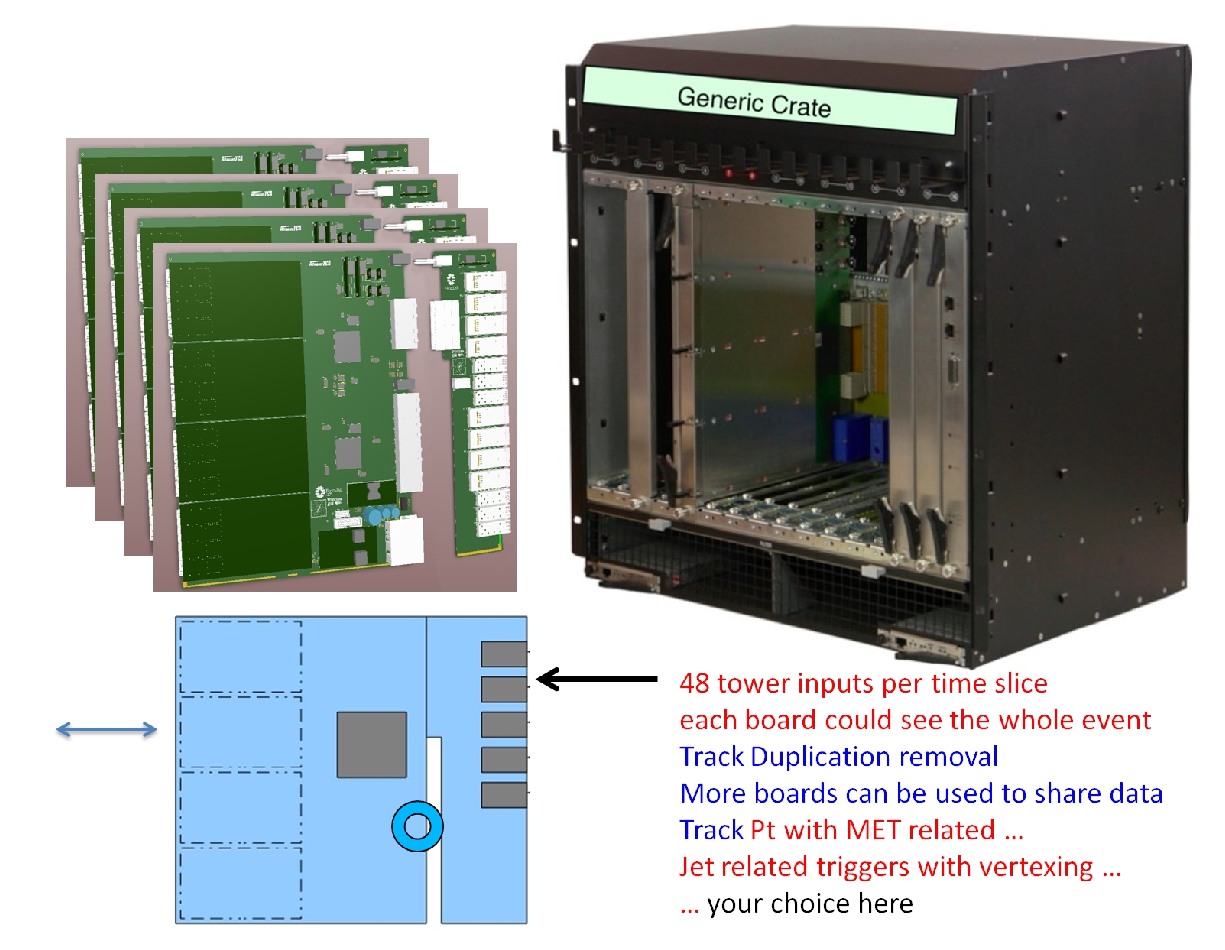
\includegraphics[width=0.5\columnwidth]{Plots/System_2.eps}
%\caption{The second processing stage shelf.}
%\label{fig:System_2}
%\end{figure}




%\begin{figure}[ht!]
%\centering
%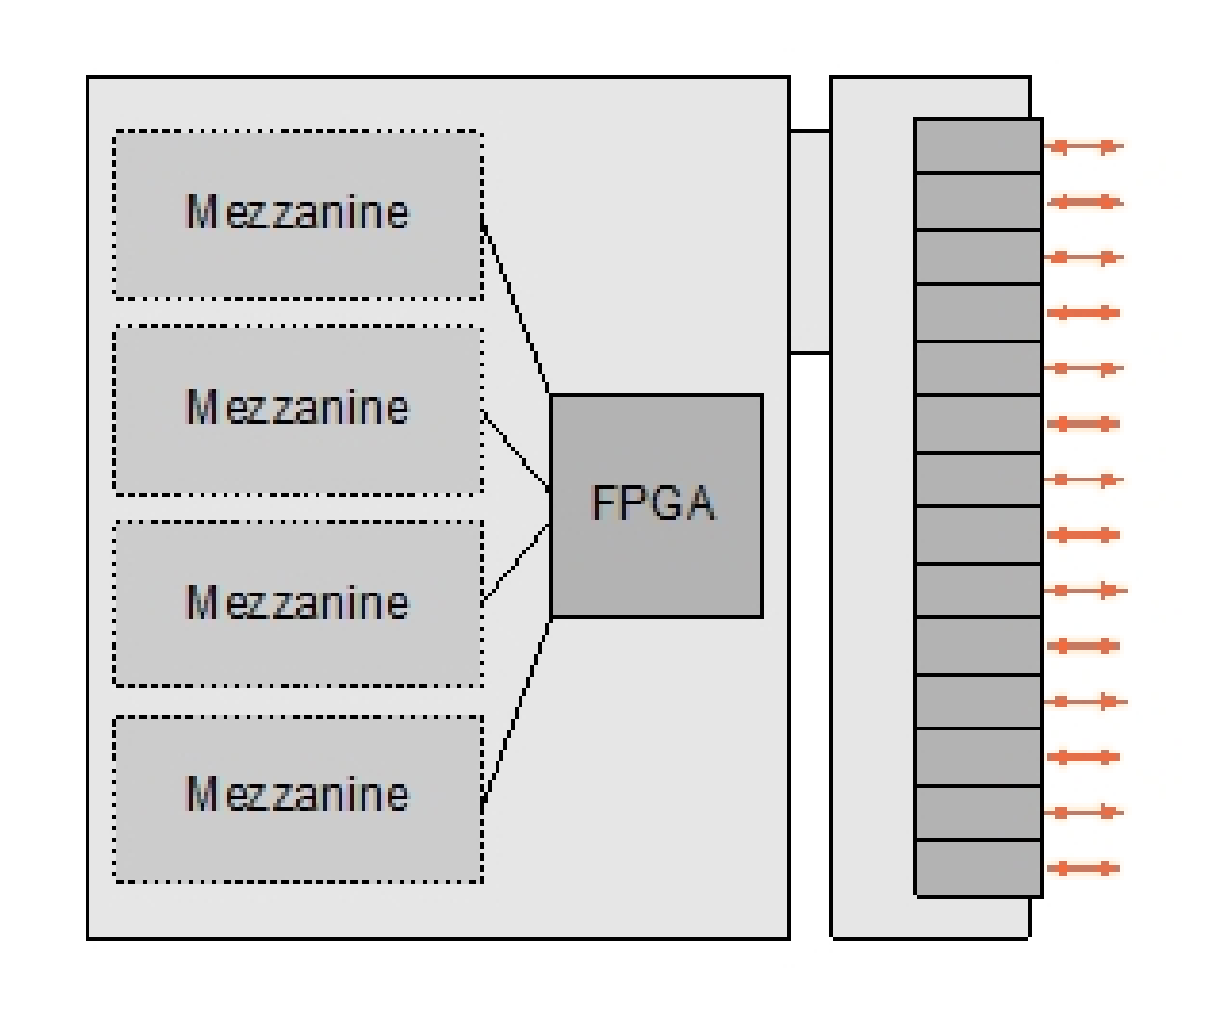
\includegraphics[width=0.4\columnwidth]{Plots/ProcBlade.eps}
%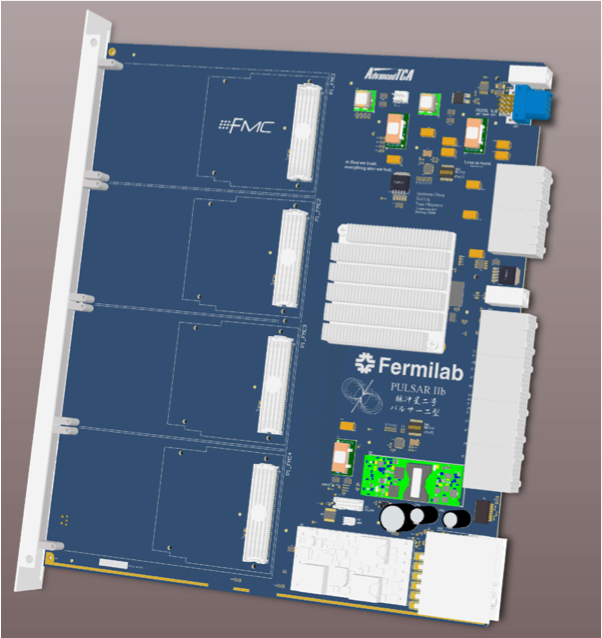
\includegraphics[width=0.4\columnwidth]{Plots/PulsarIIb.png}
%\caption{Generic processor blade concept (left), and the actual design of Pulsar %IIb~\cite{bib:PulsarII}~\cite{bib:PulsarII-weblink} at final layout stage (right)}
%\label{fig:ProcBlade}
%\end{figure}

%\begin{figure}[ht!]
%\centering
%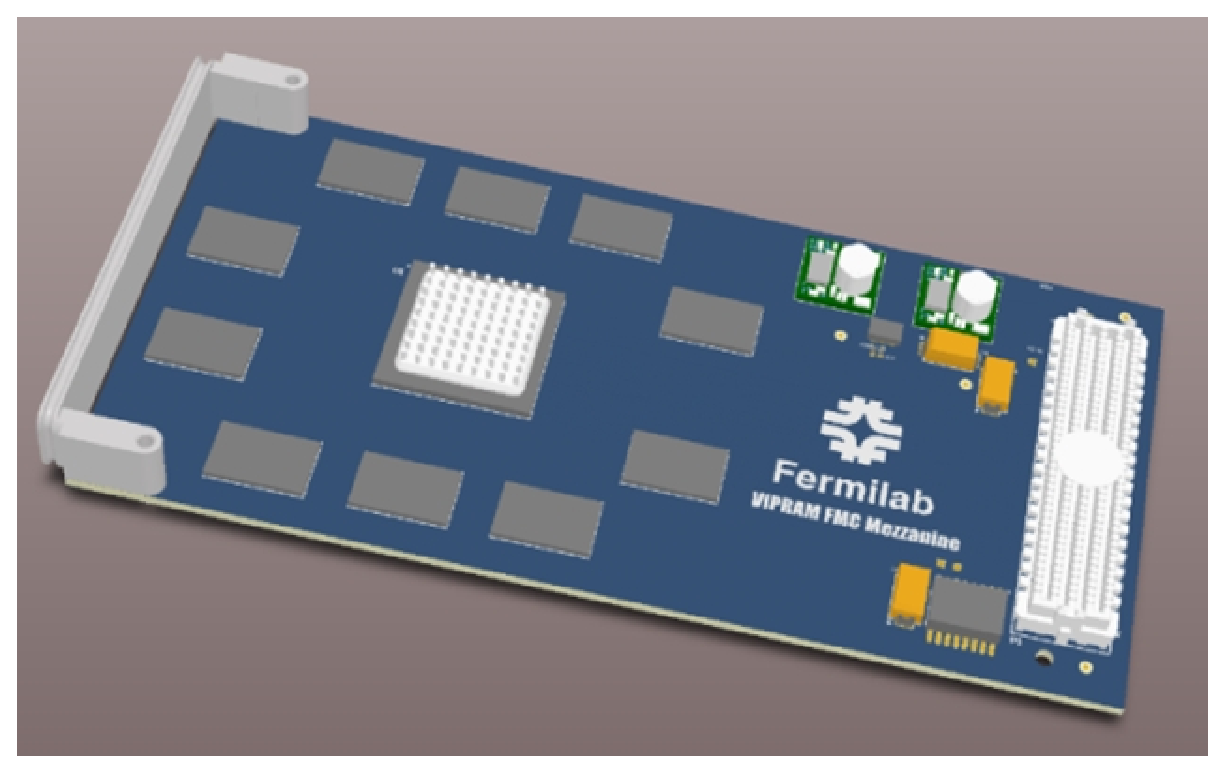
\includegraphics[width=0.4\columnwidth]{Plots/PRAM.eps}
%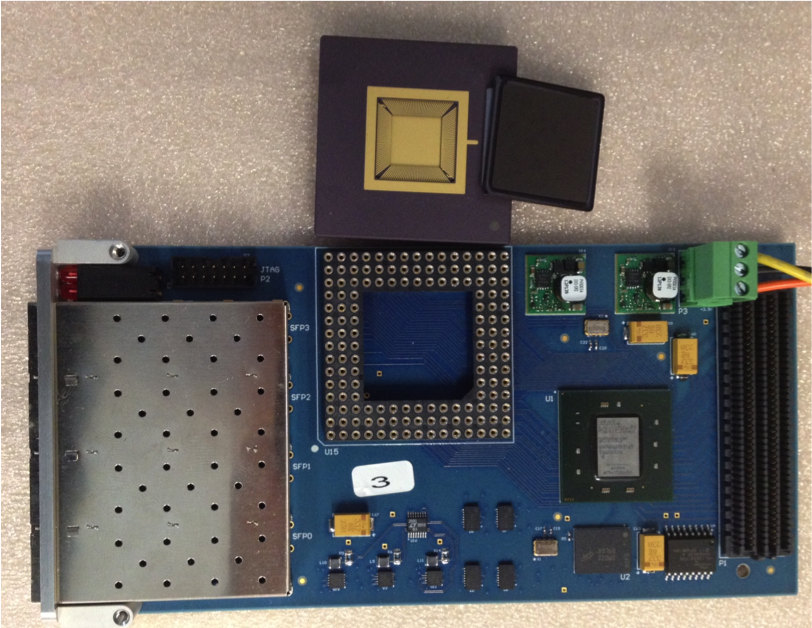
\includegraphics[width=0.4\columnwidth]{Plots/test_mezzanine.png}
%\caption{Left: Concept of a pattern recognition mezzanine design for testing different pattern recognition %algorithms.
%Right: a test mezzanine prototype designed and built at Fermilab, features four SFP+ pluggable serial %transceivers (for standalone
%data receiving), a Kintex 7 FPGA, configuration flash memory, DDR3 memory, power supplies, local %oscillators, a test socket for
%associative memory chips developed at Fermilab, and FMC connectors. 
%}
%\label{fig:PRAM}
%\end{figure}

\noindent The processor blade is the Pulsar 2b, which is shown in Figure~\ref{fig:ProcBlade}.  The front board measures 8U x 280mm and is designed around a single FPGA.  This FPGA connects directly to the full mesh backplane fabric, mezzanine cards, and fiber transceivers located on a rear transition module (RTM).  For the most part, communication channels are high speed serial point to point links and are directly supported by SERDES transceivers in the FPGA. 

\noindent The fundamental processing element or engine is a pattern recognition mezzanine (PRM) card. 
The Pulsar II supports four mezzanine cards which conform to the FPGA Mezzanine Card (FMC) standard. These mezzanine cards may contain FPGAs, pattern recognition ASICs, fiber optic transceivers, or any other custom hardware. The PRM performs both track finding and fitting. Time multiplexed data transfers into several parallel PRMs can reduce bandwidth requirement to manageable level.  PRM's using different approaches to track finding and fitting may be tested and compared within the same overall high-level system architecture and data dispatching scheme. The first prototype is shown on Figure~\ref{fig:ProcBlade} next to the Pulsar 2b.  It features four SFP+ pluggable serial transceivers (for standalone data receiving), a Kintex 7 FPGA, configuration flash memory, DDR3 memory, power supplies, local oscillators, a test socket for testing custom ASIC chips (primarily aimed at testing pattern recognition associative memory devices). This prototype mezzanine has been used extensively in FY 2014 to test the protoVIPRAM chips. Future mezzanine card designs will feature larger, more powerful FPGAs and will support multiple PRAM ASICs.  A new version of mezzanine design is in progress. 


\subsubsection{Architecture Flexibility}

\noindent

The system architecture described above is scalable, flexible and will enable us to provide an early technical demonstration of the feasibility of a L1 tracking trigger for CMS. A major advantage of the full mesh backplane is that it effectively blurs the distinction between boards, thus enabling system architects to experiment with different shelf configurations.  In the following sections we briefly illustrate two kinds of tower processor systems made possible by the flexibility of the full mesh architecture.

\paragraph{N DIB and M PRM configuration ($N+M \le 12$)}

\noindent The most straightforward tower processor architecture consists of N data input boards (DIB), which receive input links and perform zero suppression.  A DIB may be built using the generic ATCA processor blade (Figure~\ref{fig:ProcBlade}) if the data is coming from FEDs or directly from the detector modules.  
It is also possible to use a generic ATCA carrier board and several FED AMC mezzanines, if the later were to ultimately implement the DIB functionality (ie: the ability to pass stubs to the L1 track trigger PRBs).
After zero suppression, the N DIBs transfer the event data to M number of pattern recognition boards (PRB), which contain Mx4 pattern recognition mezzanine (PRM) cards.  Data transfers from the DIBs to the PRMs are time multiplexed, thus the bandwidth requirements can be significantly relaxed. For example, the bandwidth requirement for the fabric channels over the full mesh backplane can be reduced to 20 Gbps, assuming worst case scenario of 500 32-bits stubs per trigger tower per beam crossing (current studies show that on average 200 stubs are expected). 

%\noindent Data entering the PRB can be time multiplexed again and transferred to the four PRMs to further %reduce bandwidth requirements and allow for longer processing times.  The full mesh backplane fabric %supports any variant of these configurations (assuming that $N+M \le 12$), and different variants may have %different demands on hardware. Example variations are sketched on Fig.\ref{fig:System_3} and bandwidth %requirements for the worst case scenario (assuming 500 stubs per event per trigger tower) are summarized %in Table~\ref{tab:shelves}. Note that current study show that on average, we expect only about 100 to 200 %stubs per trigger tower per beam crossing, here we assumed 500 stubs to be conservative. 

%\begin{figure}[ht!]
%\centering
%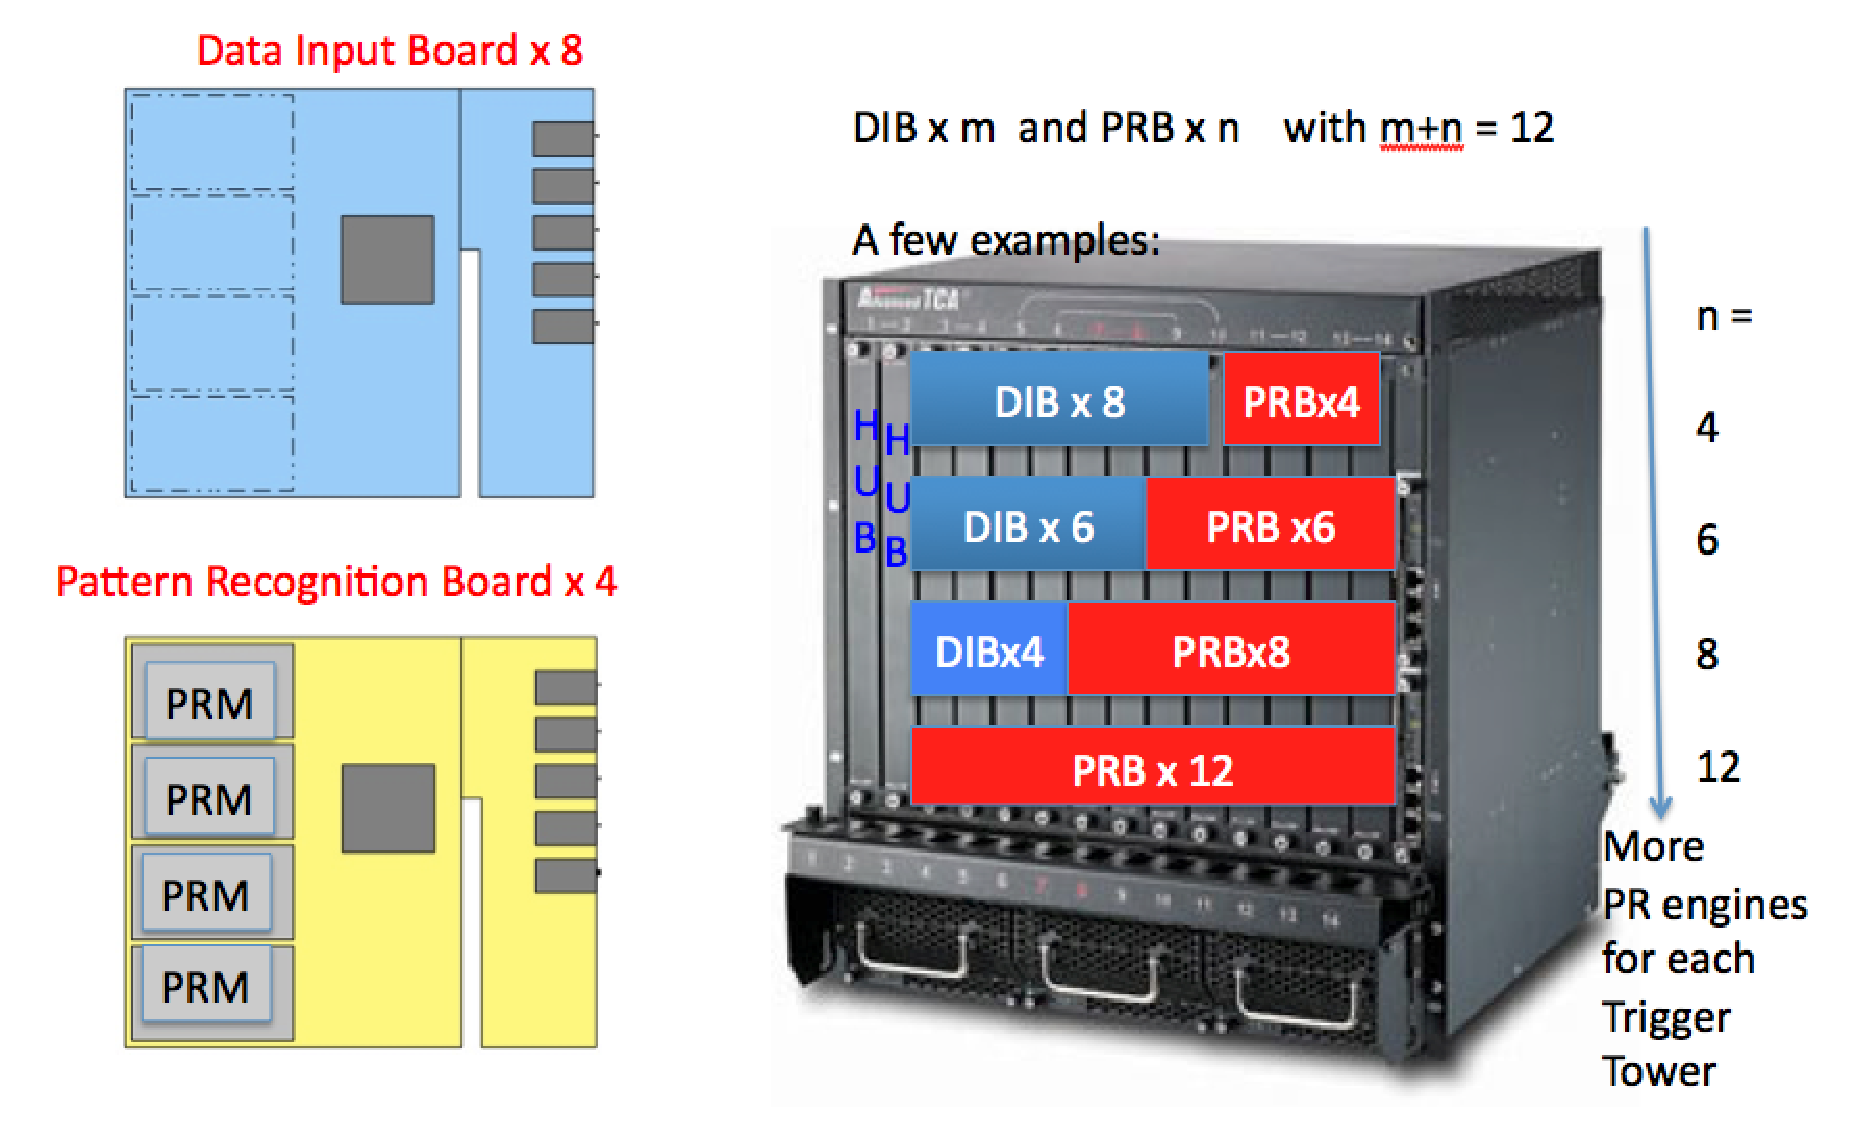
\includegraphics[width=0.7\columnwidth]{Plots/System_3.eps}
%\caption{System flexibility: many configurations possible \& being studied to select the right one for %demonstration purpose}
%\label{fig:System_3}
%\end{figure}


%\begin{table}[ht!]
%\centering\begin{tabular}{|c|c|c|c|c|}
%\hline
%DIB/PRB/PRM Count &  Fabric Channel BW (minimum)  &	PRM Input BW (minimum) \\
%8/4/16 &	20 Gbps &	40 Gbps \\
%6/6/24 &	20 Gbps &	27 Gbps \\
%4/8/32 &	20 Gbps &	20 Gbps \\
%\hline
%\end{tabular}
%\caption{Data sharing between towers occurs on the PRB board level.  Each PRB connects to the %corresponding PRB in the eight nearest tower processor shelves.  The above numbers assume a worst case %scenario of 500 32-bit stubs per trigger tower per event (every 25 ns).  An example of special configuration %with eight DIBs and four PRBs will be used as a simple example in Section 3.}
%\label{tab:shelves}
%\end{table}


\paragraph{DIB/PRB combo configuration}



%\begin{figure}[ht!]
%\centering
%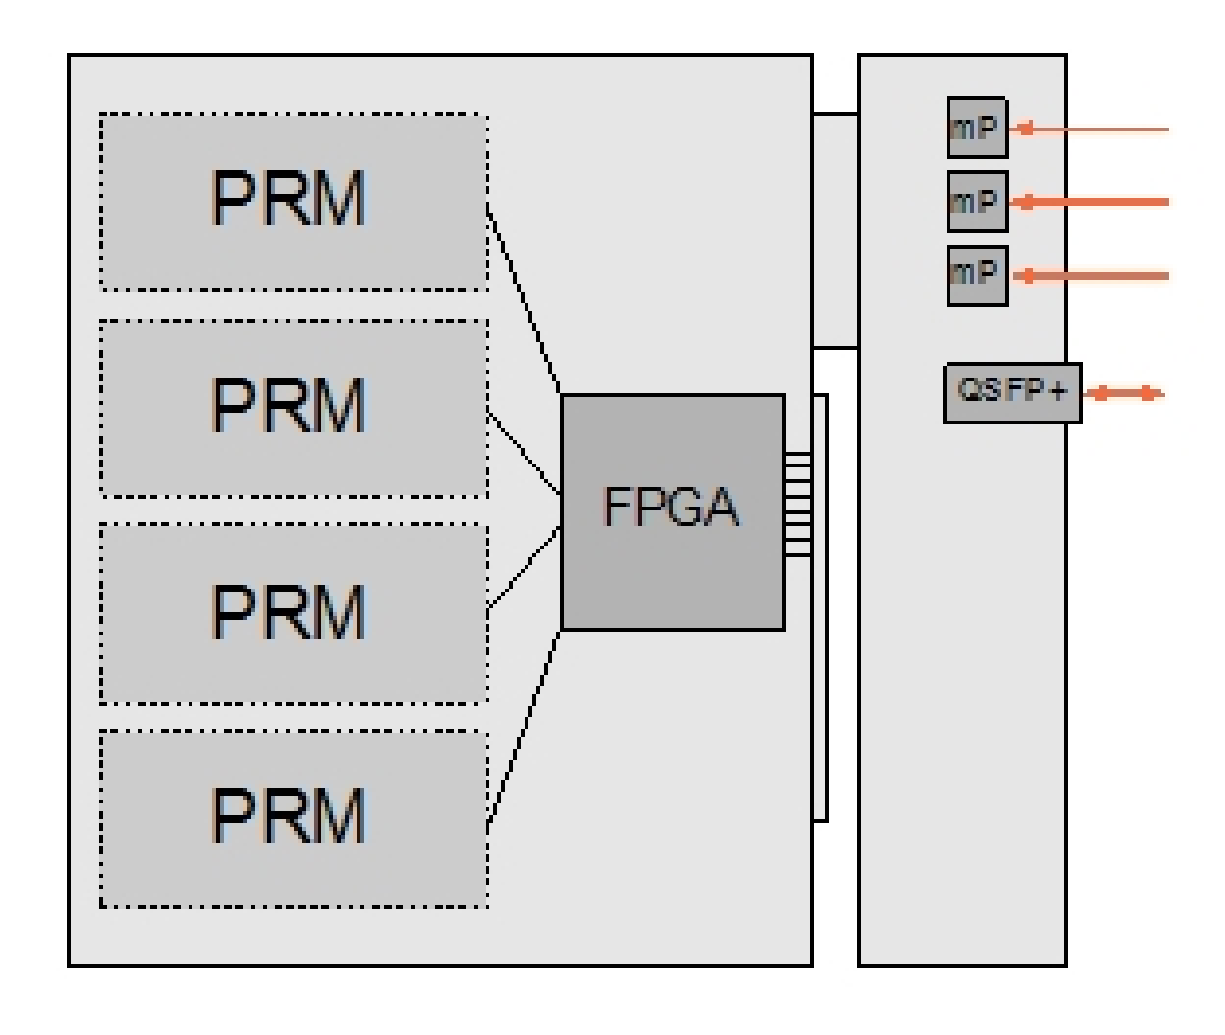
\includegraphics[width=0.45\columnwidth]{Plots/CombBlade.eps}
%\caption{Combined blade design}
%\label{fig:CombBlade}
%\end{figure}

\noindent DIB and PRB functionalities could also be combined into a single blade design, which is a special case of the "N DIB and M PRB" configuration described above (N=0 and M=12). A tower shelf would then consist of 10 Processor blades, one Gateway blade (for data sharing), and one Collector blade (for tracks found). These three different blade functionalities can be implemented in the same hardware, and Pulsar 2b is designed to meet all the requirements. The 10 Processor blades will process events in a round-robin fashion by  communicating over all available channels of the full-mesh backplane.
By using the full mesh fabric more effectively we are able to decrease the channel bandwidth requirement from 20 Gbps down to 6 Gbps with no significant latency increase. Note that Pulsar 2b has 20 Gbps fabric interface bandwidth capability, and therefore can meet the requirements in any of the system configurations described above.  


%\begin{figure}[ht!]
%\centering
%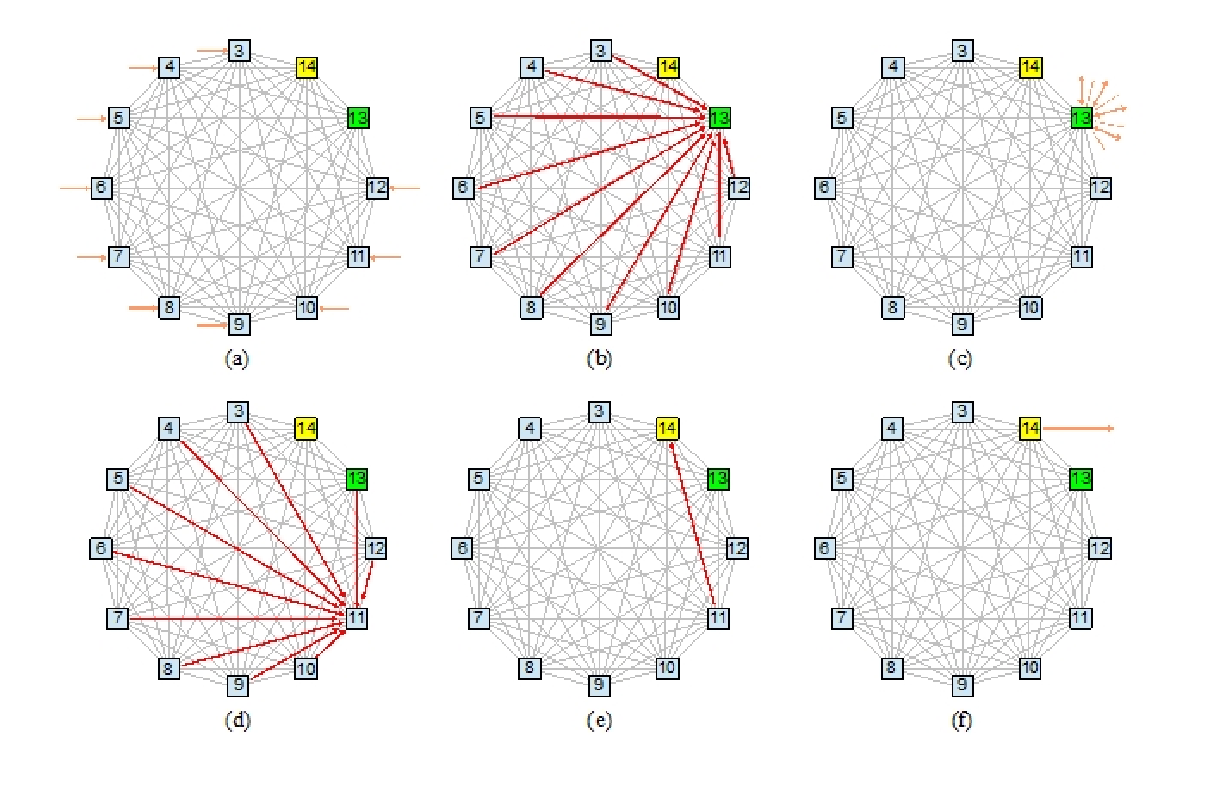
\includegraphics[width=0.9\columnwidth]{Plots/BackPlaneTr.eps}
%\caption{Backplane transfers sequences using the combined blade design. First, the input fibers are received %on the Processor blades (a).  Each Processor blade then transfers a portion of the input data to the Gateway %blade (b), where it is exchanged with neighboring towers over fiber links (c).  The Processor blades and %Gateway blade transfer the event (including neighbor data) to the target Processor blade in a time %multiplexed, round robin scheme (d).   Results from the Processor blades are then transferred to the %Collector blade (e) for any final formatting and processing before transmission downstream (f).}
%\label{fig:BackPlaneTr}
%\end{figure}
 


\subsection{Vertical Slice Demonstrator System: Overview and Methodology}

\noindent The flexible architecture described above lends itself to an early technical demonstration of the system. The main goal of the demonstration system is to identify possible problems in the architecture design and, hopefully, find solutions. We would study, measure and optimize trigger latency and efficiencies at different stages of the system using the hardware prototypes that are being developed. 
Extensive simulation work is needed to guide the hardware implementation and to establish performance expectations that can be compared with actual measurements. The proposed Vertical Slice Demonstration System is shown in Figure~\ref{fig:VS_TBench}. 

\noindent The Data Source mimics the data flow out of the upgraded Phase II outer-tracker. It will drive 300+ fibers (one/module) to the trigger tower under study exactly as if the data were coming from the real detector at high luminosity and full speed. Each fiber connection will transmit data at 3.25~Gbps payload bandwidth, i
in the same way that modules will in the Phase II Tracker. The data will be derived from simulation, appropriately formatted, stored into on-board memories, and then played back at full speed.  
The Pulsar IIb can be used for the Data Source stage, as each board has 40 optical interfaces on the RTM (all bi-drectional). Eight Puslar IIb boards can source 320 modules worth of data.

%Each stage is described in more detail in the following sections. 
%Although the architecture is flexible enough to allow for different configurations, for the sake of clarity and %simplicity, in what follows we will often use the specific configuration with eight Data Input Boards and four %Pattern Recognition Boards as an example. We will decide only at a later time which specific configuration we %will actually use for the demonstration system.

This demonstration system will be implemented in stages: at mezzanine level, board level, crate level and multi crate level. These different stages would naturally proceed in sequence, from the bottom up. This way, we will have the opportunity to learn along the way about the performance of the different components of the system before having to decide exactly how the system will be cabled. A third crate, emulating three neighbor towers, will only be introduced in the late stage of the demonstration, when studies of system dynamics are undertaken. 

\begin{figure}[ht!]
\centering
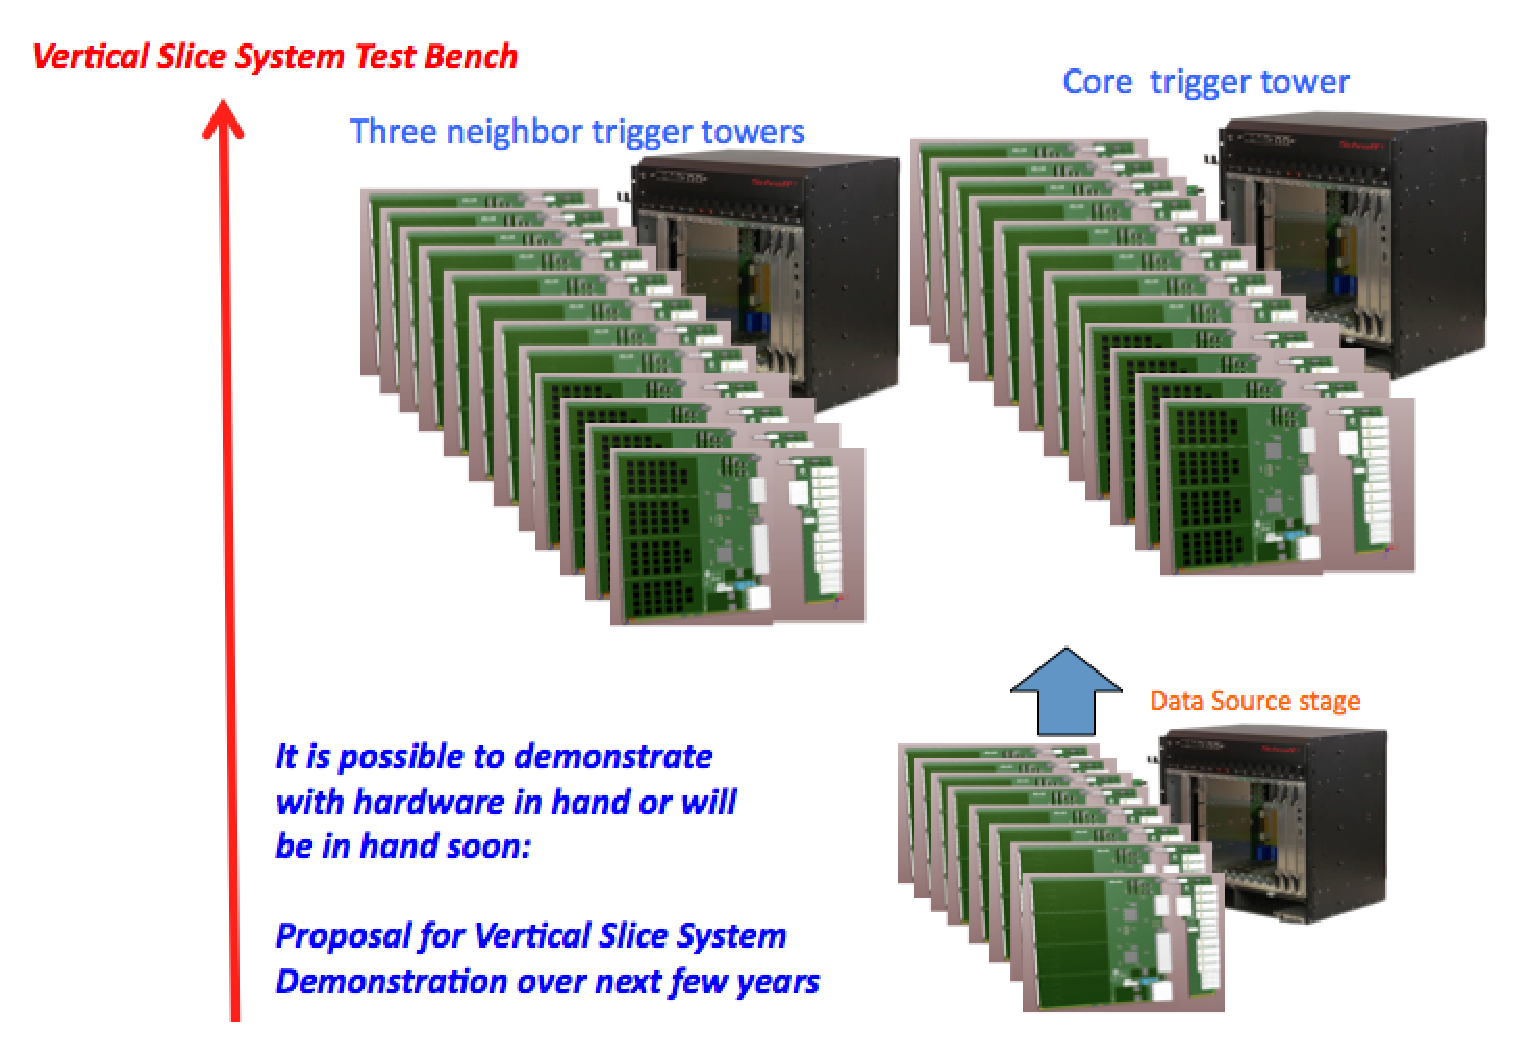
\includegraphics[width=0.8\columnwidth]{Plots/VSTBench.eps}
\caption{Vertical slice test bench principle.}
\label{fig:VS_TBench}
\end{figure}

%\subsubsection{Data Source Stage}

%\noindent The Data Source mimics the data flow out of the upgraded Phase II outer-tracker running at the %HL-LHC. It will drive 300+ fibers (one/module) to the trigger tower under study exactly as the data were %coming from the real detector at high luminosity and full speed. Each fiber connection will transmit data at %3.25~Gbps payload bandwidth, in the same way as the actual modules in the future real system. The data %will be derived from simulation, appropriately formatted, stored into on-board memories, and then played %back at full speed.  The Pulsar IIb board can be used for Data Source stage and each has 40 optical %interfaces over the RTM (all bi-drectional), and eight Puslar 2b boards can source 320 modules worth of data.

%\subsubsection{Data Input and Pattern Recognition Board}

%\noindent The Data Input Blade (DIB) is responsible for receiving data from the upstream detector %electronics (or Data Source output) and transferring them to the PRBs. Up to about 40 fiber links will be %received by each DIB. These input links may terminate on the RTM or mezzanine cards. Input fiber links are %nominally 3.25~Gb/s payload bandwidth. Again, the Pulsar IIb board can be used as DIB. The Data Input %Board will perform zero suppression, pack the stubs into a new format and send them to the PRBs. Current %estimates indicate that a rate of about 200 stubs per event per trigger tower, which yields a data rate of %roughly 256~Gb/s (200 stubs*32~bits/25~ns) entering each trigger tower on average.

%\noindent As an example, in the configuration with eight DIBs and four PRBs, each DIB will be receiving an %average of about 256/8 = 32 Gb/s of stub data (after zero suppression). Each of the eight DIBs in the shelf %sends data to four PRBs in a round-robin, time multiplexed fashion. Since data is sent to four PRBs, these %transfers can take place at a quarter of the input rate, or 32/4 = 8~Gb/s assuming 200 stubs per trigger %tower per event.

%\noindent In Figure~\ref{fig:VS_TBench}, the ATCA shelf devoted to the "core" trigger tower is shown %equipped with 8 DIB boards and 4 PRB boards while the shelf devoted to the "neighbor" towers is equipped %with 12 PRB boards, 4 PRB boards for each of the three neighbor towers. In general, each tower needs to %share data with 8 neighbors but 3 are sufficient in the demonstration system to test all possible data sharing %cases (eta, phi and "diagonal"). Simulated data corresponding to three neighbor towers are delivered from %PRB boards in the "neighbor" shelves to the corresponding PRB boards in the "core" shelf.

%\subsubsection{Pattern Recognition Board}

%\noindent Using again the special configuration above (8 DIB + 4 PRB), each PRB will be receiving 64 Gb/s %stub data on average. While receiving the data and sending them to the mezzanine cards, each PRB will %exchange data with the corresponding PRB, processing the same time slice, in the neighboring tower for %data sharing in the overlap regions. In this case, each PRB can use four 40Gb/s links (QSFP) for the %connections in the eta and phi directions, and four 10Gb/s links (SFP+) can be used for data sharing in the %"diagonal" directions. The PRB FPGA drives data received from the DIBs to the Pattern Recognition Mezzanine %(PRM) boards. This can also be done in a 4x time multiplexed fashion. The 4x time multiplexed transfers %from the PRB FPGA to the PRM would require a bandwidth of about 16Gb/s this way. Again, the Pulsar IIb %board can be used as PRB. 

 
%\begin{figure}[ht!]
%\centering
%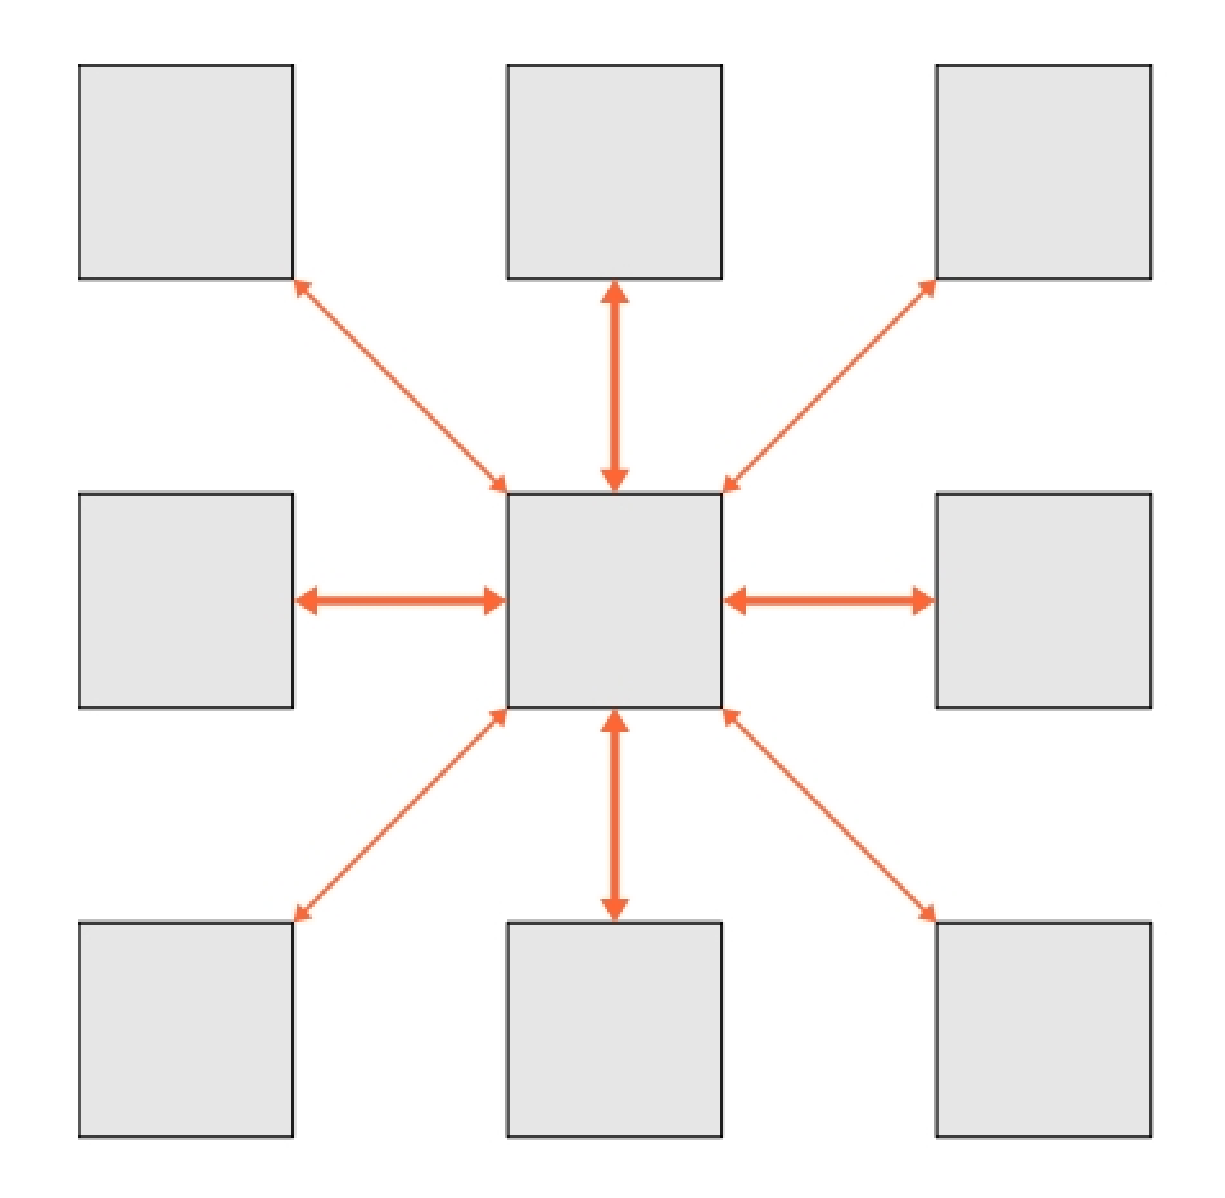
\includegraphics[width=0.4\columnwidth]{Plots/VSTBench_2.eps}
%\caption{}
%\label{fig:VS_TBench_2}
%\end{figure}


%\subsubsection{Pattern Recognition Mezzanine Card}

%\noindent Each PRB supports four Pattern Recognition Mezzanine (PRM) boards. These boards are based on %the FMC standard and support high speed LVDS and SERDES connections to the PRB FPGA. In one possible %incarnation, each PRM will contain an FPGA, on board memory to act as Data Buffer, and an array of pattern %recognition devices. In our example configuration, we need to support 16~Gb/s between the PRB FPGA and %the PRM. The FPGA-PRAM (associative memory) channel bandwidth needs will be a fraction of the PRM input %bandwidth, because only relevant stubs will be sent to the relevant pattern recognition chip covering the %relevant regions of the trigger tower.


%\begin{figure}[ht!]
%\centering
%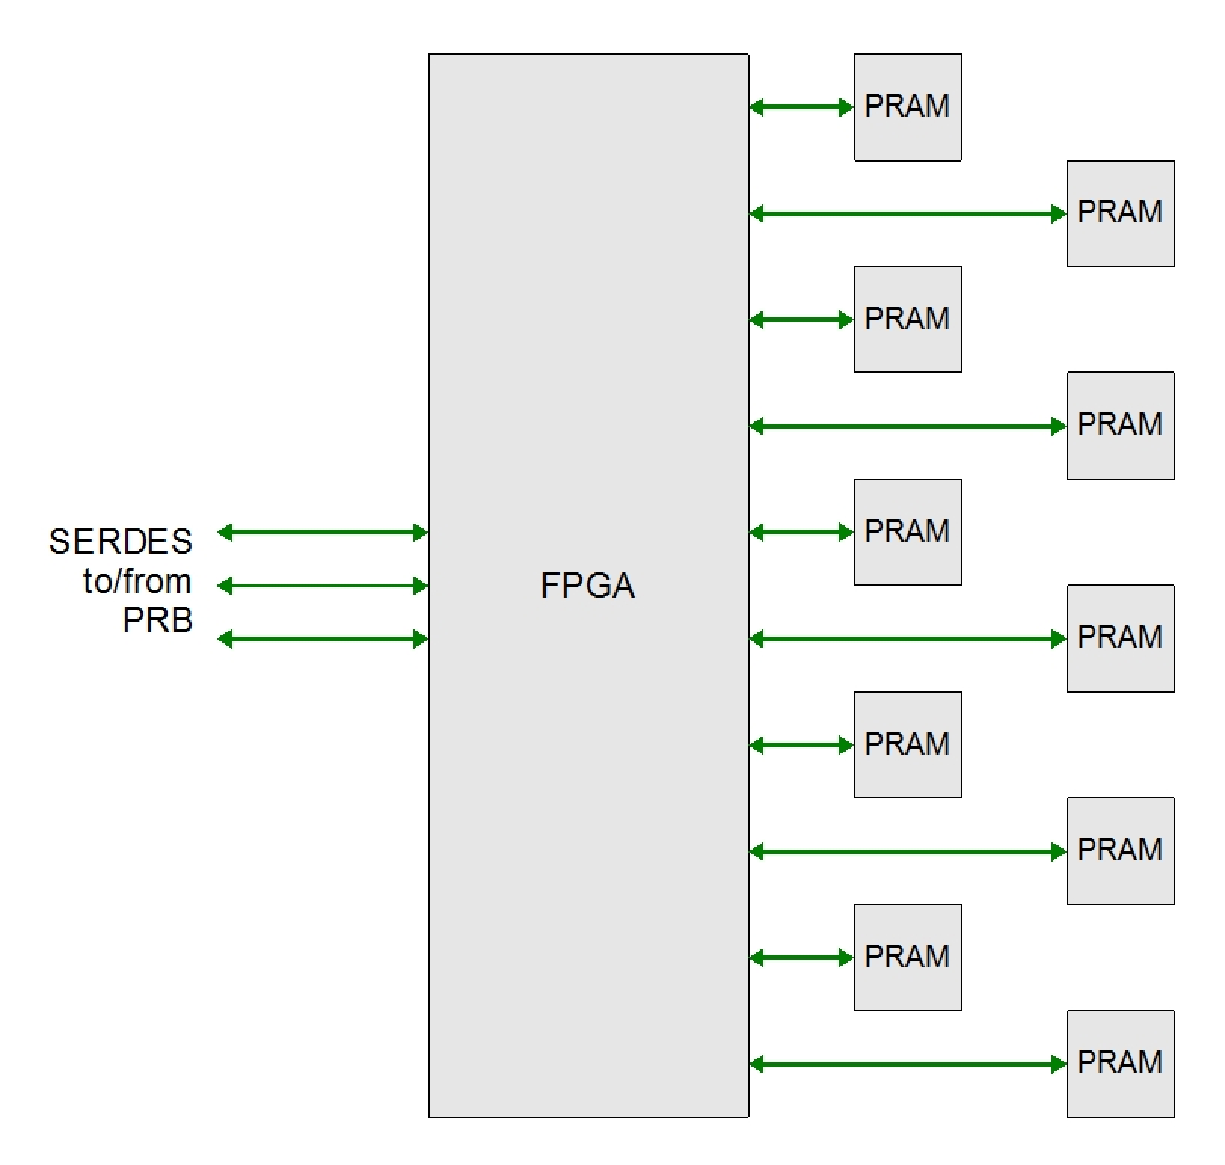
\includegraphics[width=0.6\columnwidth]{Plots/VSTBench_3.eps}
%\caption{PRM working principle}
%\label{fig:VS_TBench_3}
%\end{figure}

\noindent  
\noindent

The traditional CDF SVT/FTK-style algorithm~\cite{bib:Ann-09}  can be used to benchmark of the performance of the track fitting stage. Various experimental track fitting algorithms can also be implemented in the FPGA on the PRMs.  Each can be studied and directly compared using the same vertical slice demonstration setup.


%which is briefly described here. For a region of detector sufficiently small, a linear approximation gives helix %parameters close to those of full helical fit. In other words, for a road narrow enough that a helical fit can be %replaced by a simple linear calculation, each of the 5 helix parameters ($p_i$) can be calculated as the %vector product of prestored constants ($a_{ij}$) and the hit coordinates ($x_j$): $p_i = a_{i0} + %\sum_{i=1}^{N} a_{ij}x_{j}$  where N is the number of coordinates on the track, one for each SCT layer and %two for each pixel layer.  Since there are more than 5 coordinates, there are additional linear equations that %correspond to constraint equations, again where the constants are prestored.  There are (N - 5) such %equations. This linear approximation gives near offline resolution for regions considerably wider than a %single road.  A single set of constants will be used for each sector of the detector. The width of the sector at %each silicon layer is the size of a physical detector module.  Per sector, 5( N + 1) constants are needed for %the helix parameters, and (N - 5)( N + 1) constants are needed for the constraint equations.  The total %number of fit constants (FC) per sector is thus N(N + 1).



\section{What has been achieved in CY2014 and Plan for CY2015}


\paragraph{Pulsar II:  Pulsar IIb has been successfully tested with excellent results}

Leveraging the experience we gained through designing, building and testing the Pulsar IIa board, we have successfully designed and tested the next generation board, the Pulsar IIb (as shown in Figure~\ref{fig:ProcBlade}).
Most of the hardware design work for the Puslar II has been done in FY2014~\cite{bib:PulsarII}, including the successful design~\cite{bib:PulsarII-results}~\cite{bib:PulsarII-weblink} and testing of Pulsar IIb and its related hardware. 
The details of most recent progress report on Pulsar IIb can be found here~\cite{bib:joint-meeting}.

  The Pulsar IIb design replaces the two Kintex K325T devices with a single large Virtex-7 FPGA.  The GTH transceiver count has increased up to 80 channels, providing a significant bandwidth increase to the RTM, Fabric and Mezzanine cards. The Pulsar IIa design was originally motivated by Atlas FTK needs, but the Pulsar IIb is designed to meet the challenging requirements of CMS L1 tracking trigger demonstration. As such, the performance of the actual Pulsar IIb far exceeds the original FTK requirements. 
This includes the 80 GTH high speed (10Gbps) birectional communication channels from the Virtex-7 FPGA with challenging layout work for large ATCA board, the capability to interface with CMS TTC/FMC card, the capability to distribute TTC clock signals over the backplane so all Pulsar II based crates can run in sync with each other (important for L1 trigger applications), as well as the capability to be compatible with CMS IPBus protocol. The Pulsar IIb, as it is designed, can be used as the workhorse for the Vertical Slice Demonstration system for CMS L1 tracking trigger. The next milestone will be the full crate level testing with Pulsar IIb. Most of the Pulsar IIb design work is supported by non-CMS funds.

\begin{figure}[ht!]
\centering
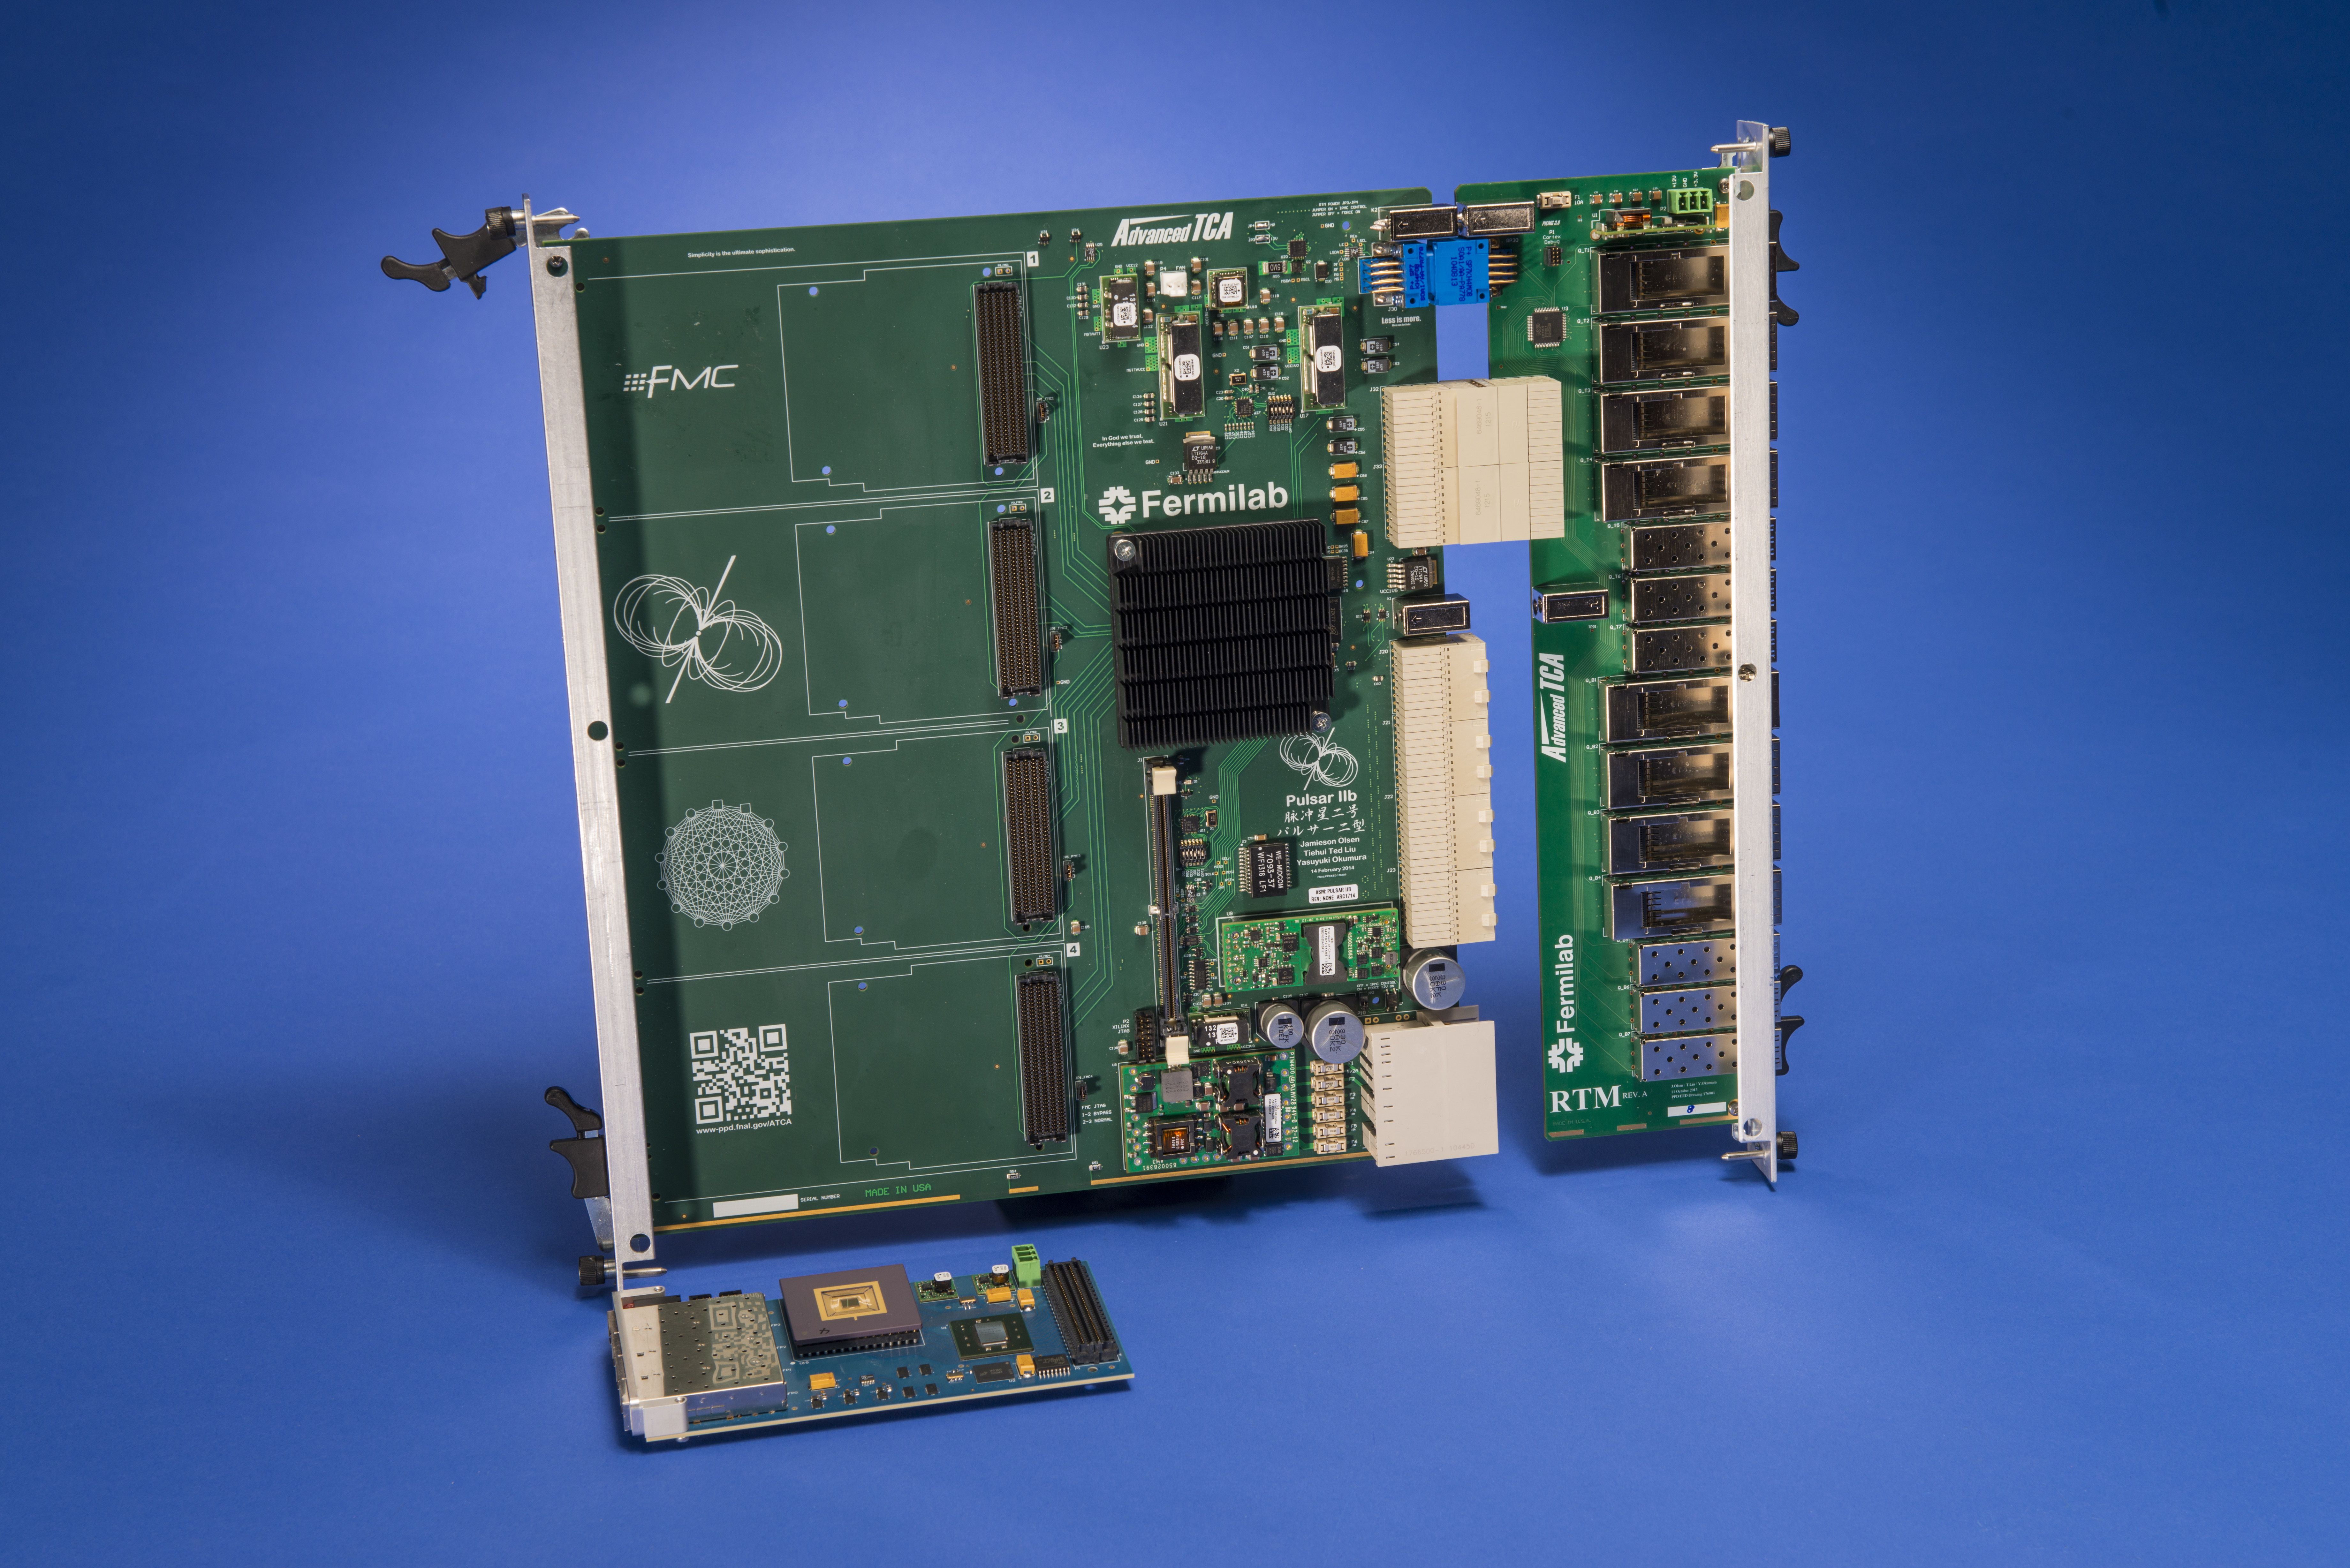
\includegraphics[width=0.8\columnwidth]{Plots/Pulsar2b-photo-compressed}
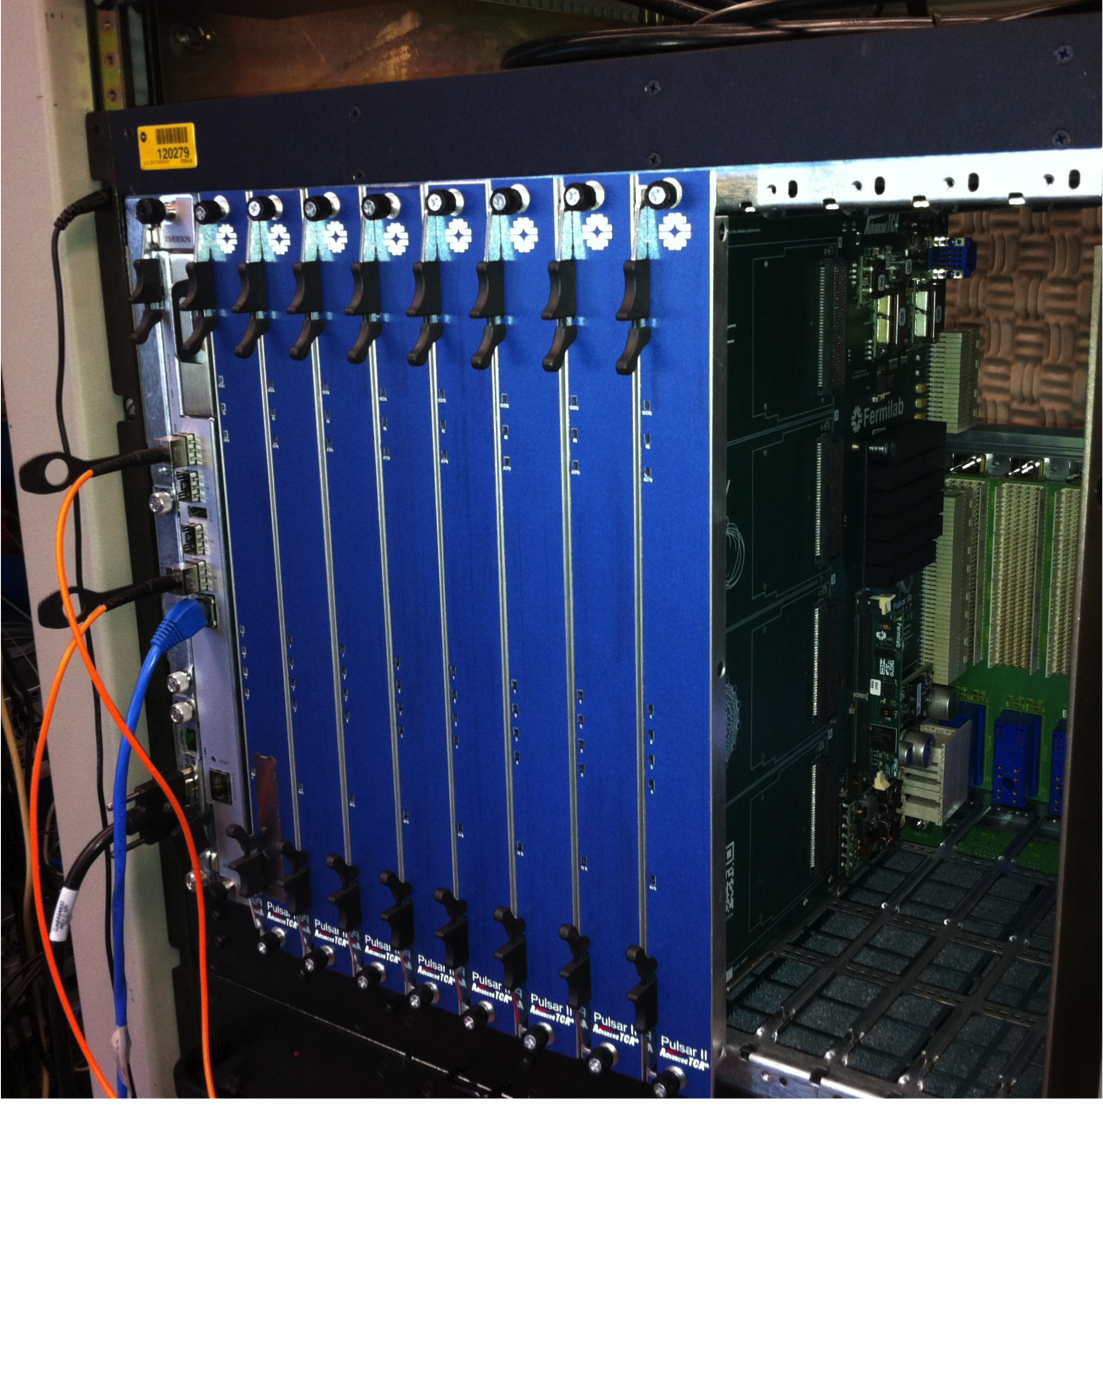
\includegraphics[width=0.2\columnwidth]{Plots/PuslarIIb-crate}
\caption{Top: The Pulsar IIb~\cite{bib:PulsarII}~\cite{bib:PulsarII-weblink} with its prototype mezzanine card.
Bottom: Pulsar IIb crate.}
\label{fig:ProcBlade}
\end{figure}


\paragraph{ATCA 40G high performance full-mesh backplane evaluation using Pulsar IIb}

Few vendors worldwide can produce ATCA shelves with a 40G high performance full-mesh backplane.
Because the Pulsar 2b fabric full-mesh performance is excellent (tested to 10 Gbps), two Pulsar IIbs are being used to evaluate the
performance of 40G ATCA crate from different vendors. The vendors are very interested in our capability to test their backplanes, and they are offering us free ATCA shelves for short term (2-3 months) evaluation purposes.  We have been testing three so far, with another due to arrive soon. Our testing results show that not all 40G full-mesh backplanes are created equal, and we will pick the best one among them.


\paragraph{Pulsar IIb new RTM, Mini-backplane, and IPMC card}

A new RTM design has been finished and submitted recently. This version has increased the channel counts from 38 to 40 (all bidirectional) to be fully compatible with the Pulsar IIb, and has improved high speed signal routing and power regulation and distribution. This version allows eight PulsarIIb boards to sink or source 320 optical links (or modules), the number of modules/fibers targeted for one trigger tower. This RTM revision work is supported by USCMS funding.

A new Mini-Backplane has been developed to loop back all fabric interface channels for high speed (10 Gbps) Pulsar IIb self testing. It also has Base Interface Ethernet ports brought out to RJ45 and SFP+, which enables single board testing on the bench top. The new mini-backplanes have been used extensively during Pulsar IIb testing, and have proven to be highly valuable.  This mini-backplane revision work is supported by USCMS funding.


An IPMC (Intelligent Platform Management Controller) mezzanine card has been developed at Fermilab. 
An IPMC is required for all ATCA boards.  The controller talks to the shelf manager to coordinate hot swap, e-keying, and to monitor various board sensors. The FNAL IPMC card has successfully powered up the Pulsar2b and RTM, and it is now part of the Pulsar IIb. This IPMC work is supported by USCMS funding.

\begin{figure}[ht!]
\centering
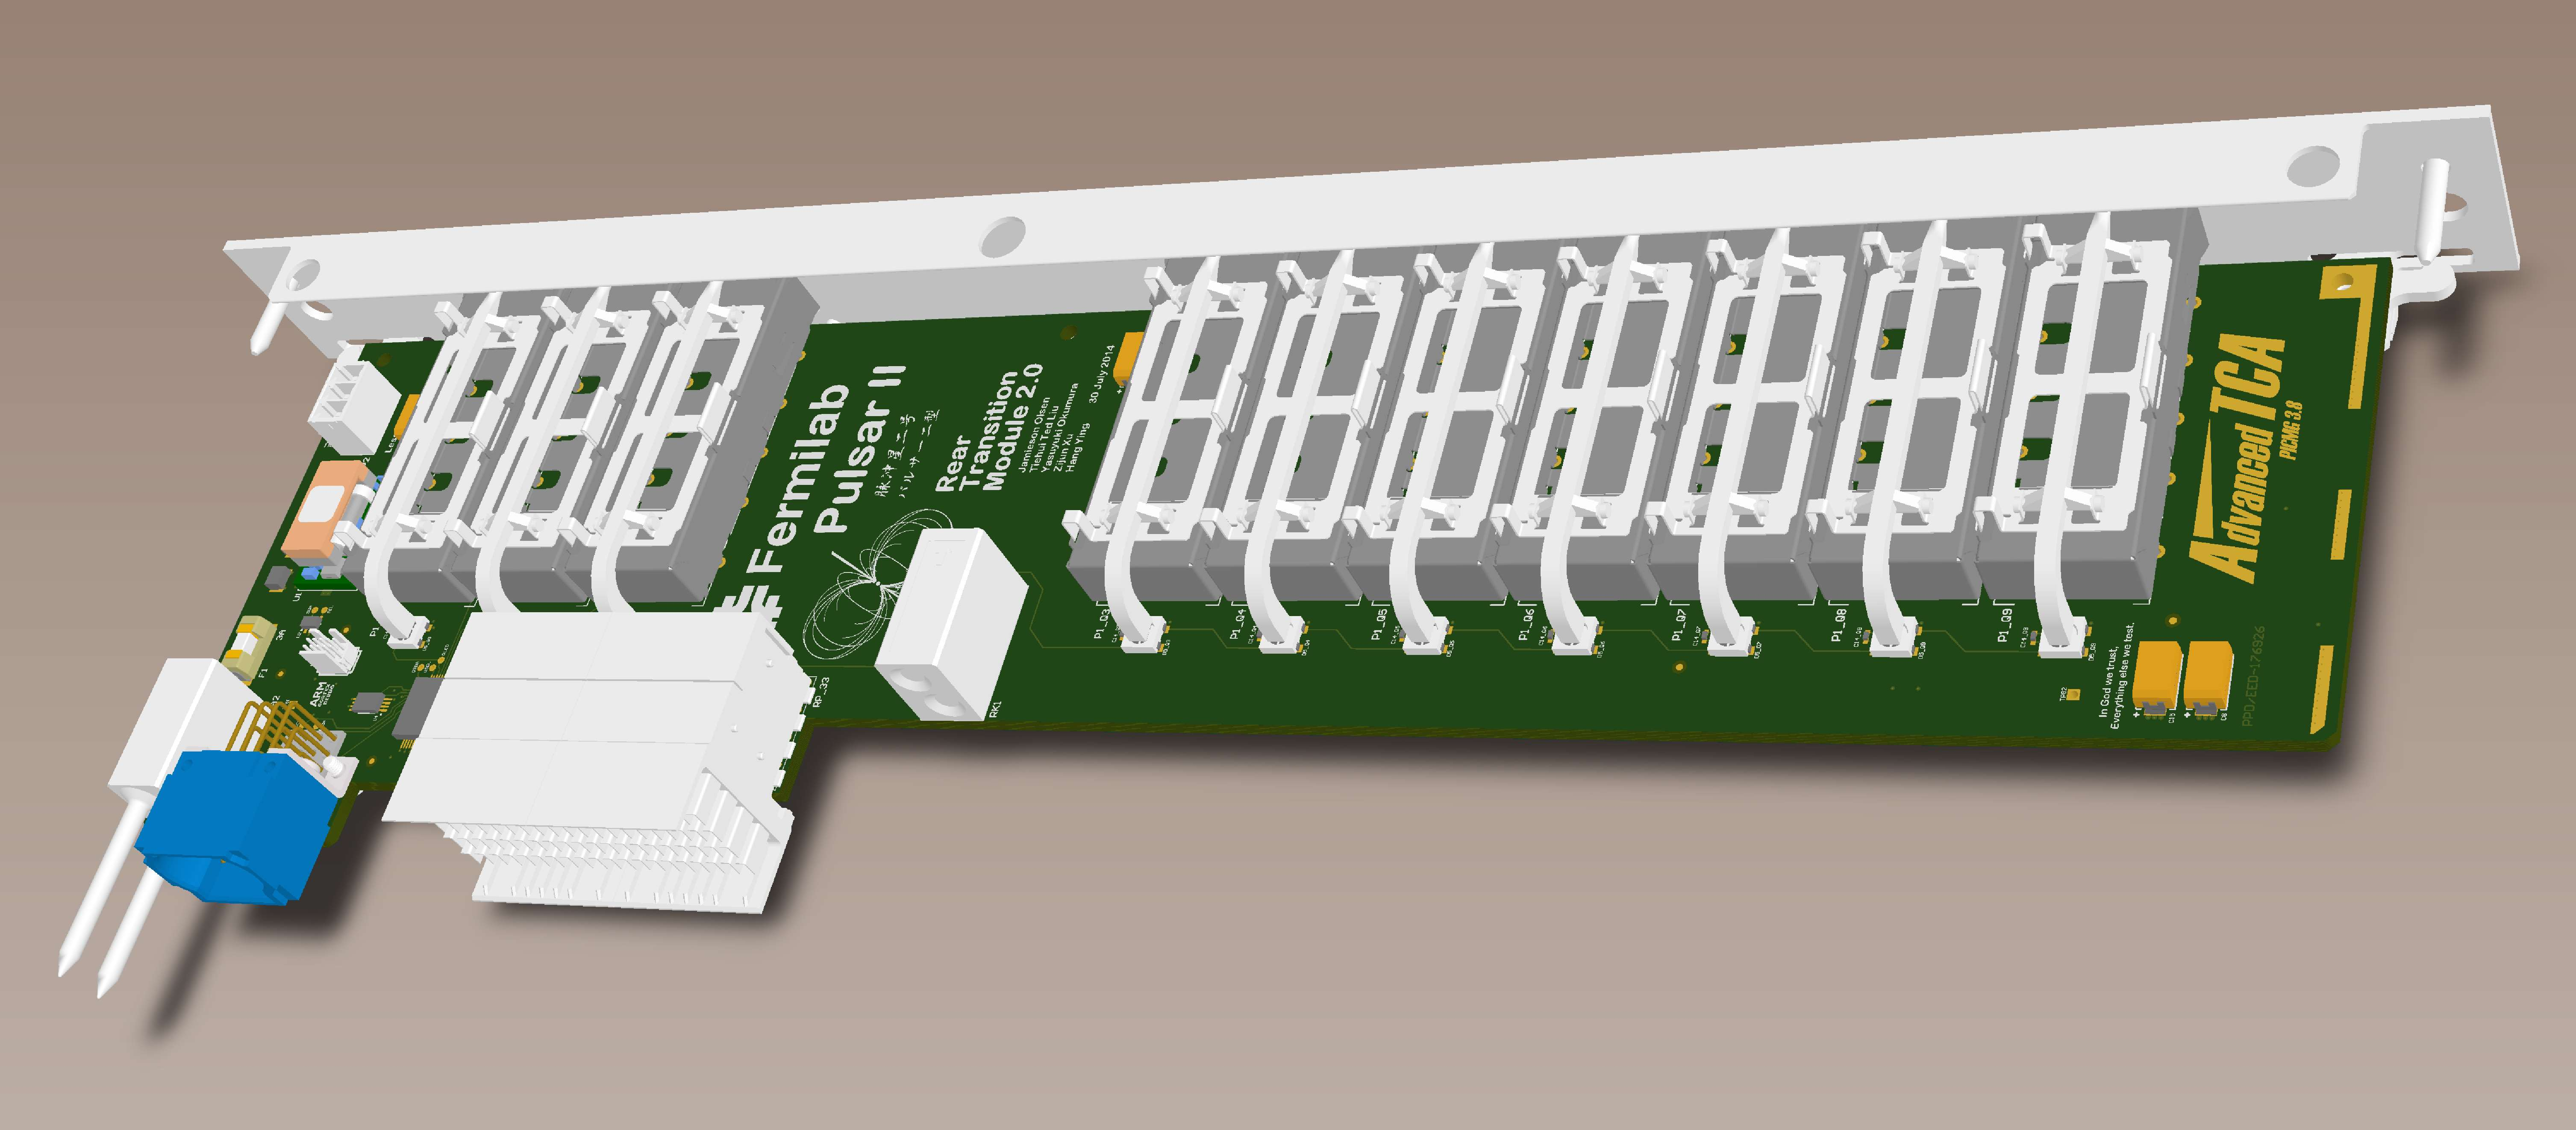
\includegraphics[width=0.8\columnwidth]{Plots/RTM_v20}
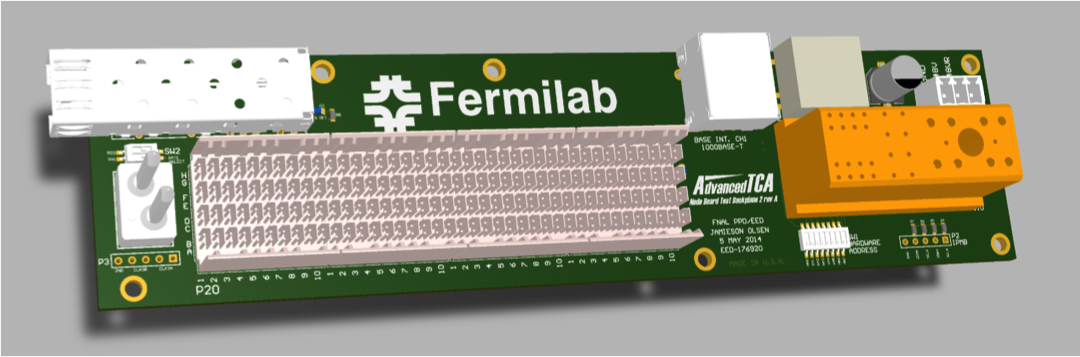
\includegraphics[width=0.4\columnwidth]{Plots/FNAL-mini-backplane.png}
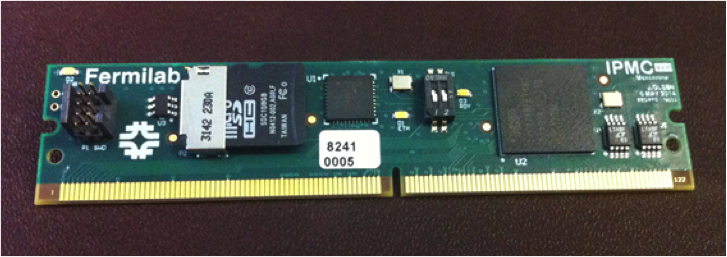
\includegraphics[width=0.4\columnwidth]{Plots/FNAL-IPMC.png}
\caption{Top: The Pulsar IIb new RTM design, just submitted. Bottom Left: Pulsar IIb new mini-backplane; Bottom Right: Pulsar IIb FNAL IPMC card.}
\label{fig:PulsarIIb-RTM}
\end{figure}



\paragraph{Next versions of Pattern Recognition Mezzanine card design in progress}

This is the core pattern recognition engine, and is being designed to host the protoVIPRAM-L1CMS chips for pattern recognition, and the latest Xilinx Ultra Scale FPGAs for high performance track fitting. This design is now in progress and will be one of the two major engineering efforts in FY2015 (the other being the protoVIPRAM-L1CMS chip design). 

Track reconstruction typically consists of two steps: pattern recognition followed by track fitting. Pattern recognition involves choosing, among all the hits present in the detector, those hits that were potentially caused by the same particle. The Associative Memory (AM) approach~\cite{bib:Rist-89} solves the combinatorial problem (due to high occupancy) inherent in this kind of pattern recognition task by employing a massively parallel architecture to simultaneously compare each detector hit to a large number of pre-calculated geometrical patterns. The AM solves the pattern recognition problem in essentially zero time, and only pass the hits of interests to track fitting stage therefore making the downstream task easier and faster.

The pattern recongition stage produces a set of hits of interest. Track fitting involves extracting track parameters from the
coordinates of these hits.  As soon as hits have been loaded in the AM, found patterns (or fired roads) are ready to be output and processed (fit) with fast FPGAs. Because each pattern corresponds to a very narrow "road” through the detector, the usual helical fit can be considerably simplified by using a pre-calculated set of parameter values for the center of the road.  Corrections are then applied as a linear function of the actual hit positions in each layer. The hits or stubs of interest within each road are combined to form tracks this way. Track helix parameters and χ2 can be extracted from the linear equations in the local silicon hit coordinates. It has been shown (by FTK and SVT) that very good performance (in terms of the resolution of the linear fit) can be achieved this way using modern FPGA DSPs. Note that the Xilinx Ultra Scale FPGAs are known for their enhanced DSP capacity, making them a suitable choice forthe pattern recognition mezzanine card.

Both the pattern recognition and track fitting stages will be implemented on the pattern recognition mezzanine card, making it the most important core pattern recogniton engine of the entire L1 tracking trigger system. The main challenge of this work is likely the firmware work due to the low latency requirement for CMS L1 tracking trigger. 

\begin{figure}[ht!]
\centering

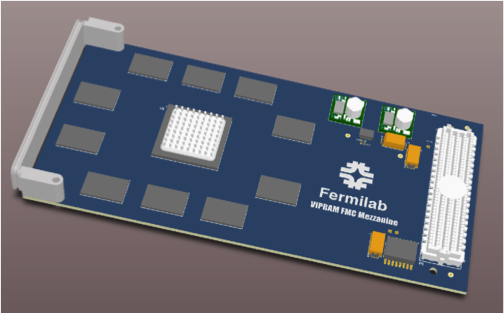
\includegraphics[width=0.6\columnwidth]{Plots/mezzanine-concept.png}
\caption{The pattern recognition mezzanine card conceptual design (compatible with Pulsar II). The new mezznine card being designed is double width mezzanine.}
\label{fig:mezzanine-concept}
\end{figure}


\paragraph{VIPRAM R\&D: ProtoVIPRAM 2D chip has been successfully tested}

The numerous advantages of an Associative Memory-based track trigger are well established.  Its primary limitations lie in pattern density and in readout speed for Level 1 trigger applications.  A secondary challenge is to minimize power consumption.  Vertical Integration is an emerging technology which offers dramatic improvements in all these areas.  The overall objective of the VIPRAM project at this point is to make steady progress towards a final solution.  This requires a strategic approach to architecture and layout that permits near term solutions in classical VLSI technology and long term solutions in aggressive Vertical Integration. 

From the beginning, our design methodology has been to develop concepts and circuitry in 2D to confirm functionality as economically as possible and then to translate, where necessary, those ideas into 3D.  The first step taken by the VIPRAM Project was the development of a 2D prototype (protoVIPRAM1) in which the associative memory building blocks were laid out as if this was a 3D design.  Room was left for as yet non-existent Through Silicon Vias and routing was performed to avoid these areas.  
%In protoVIPRAM1, there are four independent but identical CAM cells for each Control cell arranged into a unit called a protoLeg.  Each protoLeg %contains all the memory, comparison circuitry and evaluation logic necessary to perform the pattern recognition algorithm for one complete 4-layer %road.  protoVIPRAM1 is an array of 32 by 128 protoLeg cells.  
The readout circuitry is deliberately simplified to allow direct performance studies of the CAM and Control cells.  The protoVIPRAM1 was designed and fabricated in a 130nm Low Power CMOS process.  The design was thoroughly simulated at all levels before submission and the teststand was fully ready before the chips arrived. In fact, we were able to correctly observe found patterns the day after the first prototype chip became available for testing. 

The first prototypes of the protoVIPRAM verifies the CAM and majority logic designs for future use in more application specific chips. The testing results match the simulation studies and show that these building blocks are ready for 3D stacking.  The results have been presented at the Front-end electronics workshop (FEE 2014).  More detailed testing results of the prototype will be presented at TWEPP 2014. This work is supported by DOE CDRD funds.


\begin{figure}[ht!]
\centering
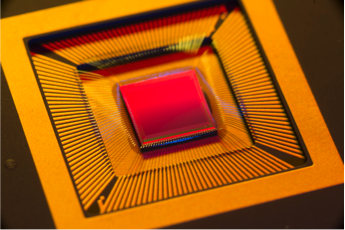
\includegraphics[width=0.3\columnwidth]{Plots/ProtoVIPRAM-photo.png}
\includegraphics[width=0.6\columnwidth]{Plots/ProtoVIPRAM-mezzanine.png}
\caption{The protoVIPRAM and its testing mezzanine card (compatible with Pulsar II). This prototype mezzanine has been used extensively in FY 2014 to test the protoVIPRAM chips.}
\label{fig:ProtoVIPRAM}
\end{figure}


\paragraph{VIPRAM R\&D: Next versions of ProtoVIPRAM design in progress}

The VIPRAM approach has, from the beginning, attempted to increase pattern density and decrease power density through Vertical Integration.   To mitigate issues implicit in adopting an emerging technology, a flexible architecture has been developed that can be implemented in either conventional or Vertically Integrated VLSI.  This allows us to bring the system interface to maturity at an early stage while, at the same time, making steady progress towards the final VIPRAM solution.  This is particularly important for Level 1 Tracking Trigger applications. The protoVIPRAM1 is the first step to developing the next generation AM chips for L1 applications. 
The next two steps will be performed in parallel. We now have two designs in progress:  protoVIPRAM3D and protoVIPRAM-L1CMS.

The protoVIPRAM3D takes the circuitry designed in protoVIPRAM1 and vertically integrates it.  The Control cells are moved onto a Control Tier and the CAM cells become a CAM Tier.  Since the basic building blocks are already fully tested in 2D, what we will be testing with protoVIPRAM3D is the 3D design and process. The chip interface will be kept the same as the protoVIPRAM1, so that the testing can be done in the same way, allowing us to compare directly the 3D version performance with that of the 2D. This work is supported by DOE CDRD funds.

The protoVIPRAM-L1CMS for CMS, on the other hand, attempts to improve the data input and readout speed of the associative memory chips and bring the system-level interface to maturity using conventional 2D VLSI. The flow of VIPRAM’s tasks can be divided into two broad categories: 1) Pattern Recognition Associative Memory (PRAM), and 2) input/output and control (IOC).  The former consists of CAM Cells, Majority Logic Cells, and pattern and critical signal distributions.  This was the focus of protoVIPRAM1, a 2D implementation of the 3D-compatible cells necessary for the final design.  The IOC consists of data input handling, slow control, road match capture, sparsification, and road output.  During operation, silicon data is sent to the VIPRAM followed by a unique End-of-Event signal.  At the arrival of the End-of-Event, the road match capture logic in the IOC snaps a picture of the state of the PRAM, freeing the PRAM to begin collecting data for the next event, if necessary.  The captured road match snap shot is sparsified, placed in a FIFO, serialized and driven off-chip to the track fitting logic.

Design in Vertical Integration is, in a sense, the logical partitioning of functionality into a third dimension. To make an architecture that can be either 2D or simple 3D or more aggressive 3D, the partitioning must also be adjustable so that its granularity can be changed to fit the desired implementation with the present available technology in a cost effective way.  The PRAM structure, intrinsically, is adjustable in the 3rd dimension from the full road level down to the individual CAM level.  The IOC, being logically separable from the PRAM, can be implemented on its own tier as well, leaving more space for a high performance system interface. This flexible architecture is fully compatible with our long-term goal of high-density 3D stacking while, at the same time, achieving our near-term need of a functional chip for a CMS Level 1 Tracking Trigger demonstration.

This design is dedicated for CMS Level 1 trigger applications.  Several of the ideas introduced in the protoVIPRAM1, most notably the square layout of the CAM cells and the simplified readout architecture, will be used as stepping stones for increasing readout speed and flexibility. For example, Figure~\ref{fig:protoVIPRAM-L1CMS-pattern} (right) is the layout of the 8-layer pattern core of protoVIPRAM-L1CMS, which is the basic building block that includes all circuitry necessary to match layer addresses to pattern addresses and then to associate matched addresses to road matches.  It is approximately 1600 transistors in an area of 70x70 microns.  
%Address data comes from all sides.  For example, layer 1 and layer 2 address data comes from the right, layer 3 and layer 4 address %data comes from the bottom, etc.  This not only distributes the power consumption in the periphery uniformly, but it also allows us to %spread the sense lines apart, reducing sidewall capacitance and increasing speed.  
This pattern footprint size allows us to connect it to the readout architecture either by 3D methods or by classical bump bonding.  The image shown is for 3D Direct Bond Interconnect (3DDBI).  This is indicated by the array of small octagons across the pattern block.  Note that configuring this for bump bonding does not require a new layout.  Foundries permit extra wafers to be fabricated using metal redistribution (RDL) layers for bump bonding.  In short, the same mask set can fulfill more than one objective. The protoVIPRAM-L1CMS design is supported by USCMS funding. 




\begin{figure}[ht!]
\centering
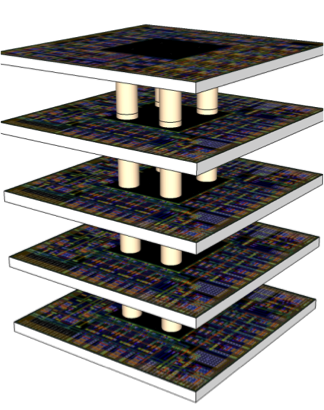
\includegraphics[width=0.2\columnwidth]{Plots/VIPRAM-3D.png}
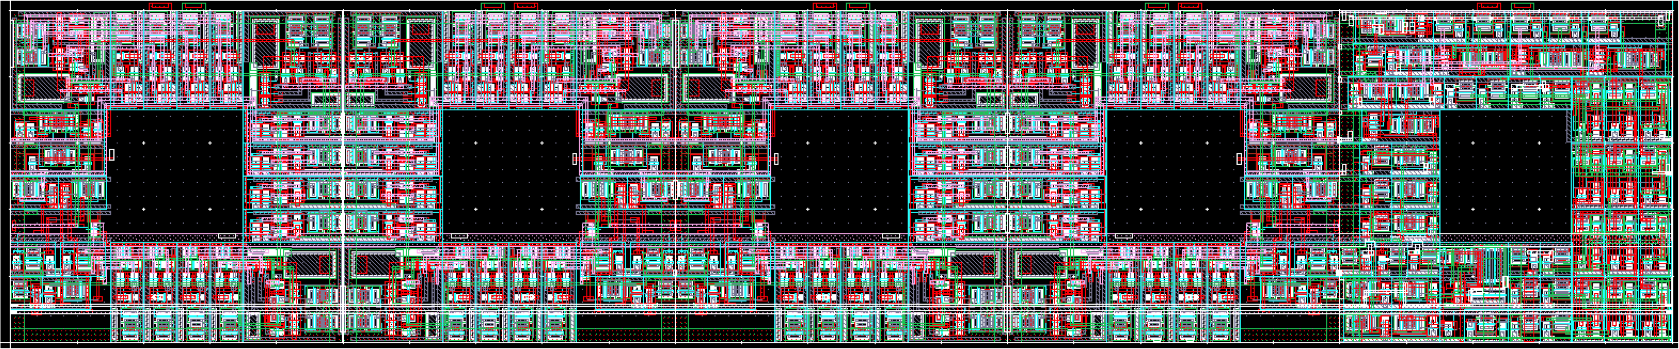
\includegraphics[width=0.3\columnwidth]{Plots/protoVIPRAM-2D.png}
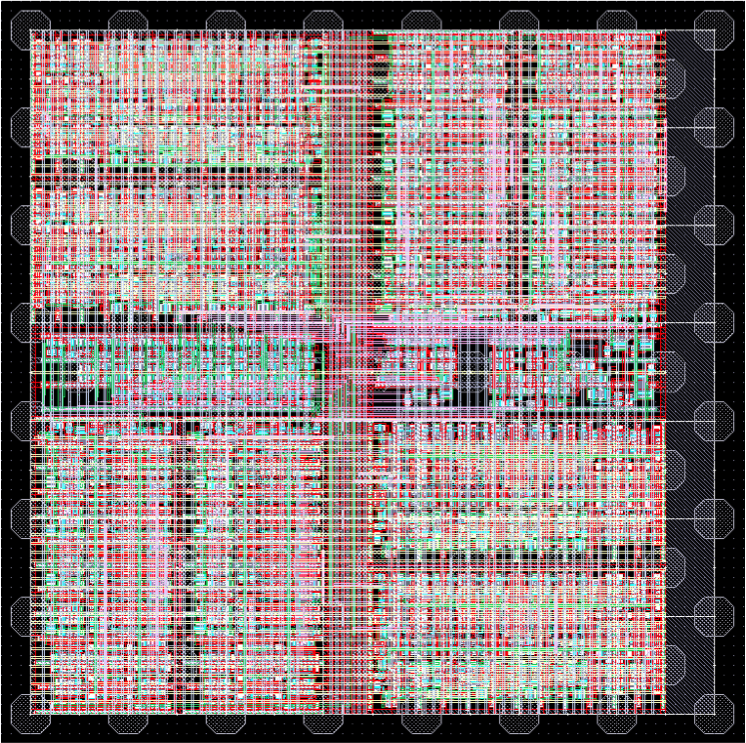
\includegraphics[width=0.2\columnwidth]{Plots/protoVIPRAM-L1CMS-pattern.png}
\caption{Left: We started with a 3D VIPRAM concept~\cite{bib:VIP-11} a few years ago and followed with a generic R\&D project~\cite{bib:VIP-12} funded by DOE CDRD.
Middle:  The first step taken was a 2D prototype (protoVIPRAM1) in which the associative memory building blocks were laid out in 2D as if this was a 3D design. A four layer AM pattern design in 130 nm for protoVIPRAM1, with a layout footprint of 25um X 125um size.
Room was left in the middle for as yet non-existent Through Silicon Vias and routing was performed to avoid these areas.
Right: One full eight layer AM pattern design in 130 nm for protoVIPRAM-L1CMS, with 70um x 70um size. Note there is no room left for TSVs in this case. One can then tile these pattern blocks on one tier uniformally, and have readout of fired roads on the second tier. The two tiers can be connected either via conventional bump bonding, or using the 3D DBI technology. Current plan is to have the design compatible with both approaches.}
\label{fig:protoVIPRAM-L1CMS-pattern}
\end{figure}

Both designs are in progress in CY2014 and will continue into CY2015, with chip submission expected in CY2015. Both designs will be on the same MPW run. To realize substantial savings in fabrication costs, protoVIPRAM-L1CMS will share wafer space with two additional chips being developed at Fermilab. One is our own protoVIPRAM3D, the other is the VIPIC (Vertically Integrated Photon Imaging Chip) designed to address the challenges of X-ray Correlation Spectroscopy (XCS). The VIPIC project is funded by BES.
Figure~\ref{fig:VIPRAM-MPW} shows the division 2:1:2 (area ratio) of a reticle between the protoVIPRAM-L1CMS (HEP/CMS), protoVIPRAM3D (HEP) and VIPIC (BES) projects on the planned 3D run. The total cost of the MPW is \$450K, and protoVIPRAM-L1CMS share is \$180K while the protoVIPRAM3D is \$90K. The protoVIPRAM3D work is supported by generic R\&D funds so far. 
The processing cost following the wafer stage is \$80K for protoVIPRAM-L1CMS, bringing the total cost to \$260K. We are requesting USCMS funds to cover the cost for protoVIPRAM-L1CMS.

\begin{figure}[ht!]
\centering
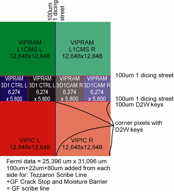
\includegraphics[width=0.35\columnwidth]{Plots/VIPRAM-MPW.png}
\caption{A drawing showing the division of a reticle between the VIPRAM (HEP) and VIPIC (BES) projects on the planned 3D run.
}
\label{fig:VIPRAM-MPW}
\end{figure}




\paragraph{Fermilab URA fellowships for VIPRAM R\&D and engineering students}

Last year, one URA fellowship was awarded to SMU Electrical Engineering graduate student for one year to work on the power and thermal analysis of the protoVIPRAM design. The work done by the student (from Prof. Ping Gui's group) 
has laid the foundation for the power and thermal analysis of the chip. This year another URA fellowship was awarded to Northwestern Electrical Engineering graduate student (from Prof. Seda Memik's group) to continue this work for one more year, this time with an emphasis on the protoVIPRAM3D power and thermal analysis. In addition, one visiting engineering student from BIST/India worked on
VIPRAM project for more than one year with extensive simulation and testing work done for the VIPRAM project.
This work was supported by generic R\&D funding. Over the past year, there has been three engneering master degree theses on VIPRAM. 

\paragraph{Work done by the Northwestern group}

The Northwestern group (lead by K. Hahn) has made significant progress over the past year on key aspects of system integration and data formatting/transfer.  Their integration efforts include the development of IPBus firmware and software for the Pulsar II based ATCA platform.  IPBus is a flexible, scalable application layer protocol that will become the primary means of DAQ/trigger slow control in Phase-2.  The group has developed a functioning implementation of IPBus firmware for both the Pulsar 2a and 2b, and has demonstrated control of Pulsar hardware with IPBus routed through a commercial ATCA switch.  The group's IPBus implementation is an important milestone for the AM-based Tracking Trigger project, and has facilitated the testing of AM prototypes at FNAL.

Northwestern is additionally developing and testing firmware that will integrate the Pulsar platform with the CMS/LHC TCDS system.  The firmware enables the Pulsar to receive LHC signals and clock and to distribute these within the ATCA shelf.  The team has successfully tested a basic version of the firmware with a $\mu\rm TCA$ GLIB and a legacy TTC system at CERN.  Their effort is now focused on transitioning the firmware to the Pulsar hardware.  A demonstration of TTC distribution over ATCA will be jointly conducted by Northwestern and FNAL at CERN in the near future.

With regard to data transfer, the Northwestern group is performing an extensive evaluation of the Aurora family of protocols from Xilinx.  These protocols are an industry-standard for low-latency, multi-gigabit serial communication.  The team is assessing the suitability of Aurora for application in the L1 trigger environment by simultaneously characterizing link latency and signal integrity.  Northwestern has shown that the Aurora 8b/10b protocol can be used to achieve $\sim130\rm~ns$ latency for point-to-point Pulsar communication over the ATCA backplane (Figure~\ref{fig:scope}).  The team has recently embedded a microblaze soft-processor in their Aurora test-bench to enable the in-system collection of link quality statistics as a function of transceiver/protocol configuration.


%-----------------------------------------------------------------
\begin{figure}[h]
\begin{center}
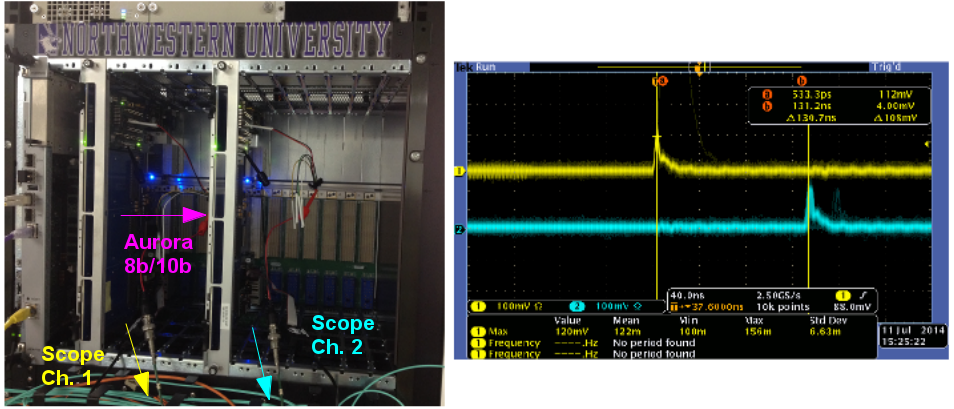
\includegraphics[width=0.80\linewidth]{Plots/crate_and_scope.png}
\caption{Left: Northwestern ATCA test-stand configured for Aurora link testing.  Right: scope trace showing $\sim 130\rm~ns$ latency for Aurora 8b/10b Pulsar-to-Pulsar communication over the ATCA backplane.}
\label{fig:scope}
\end{center}
\end{figure}
%-----------------------------------------------------------------

Northwestern has designed and proposed a data formatting scheme for the communication of stubs from the Tracker front-end to and within the Pulsar II ATCA-based trigger towers.  The proposed format was recently endorsed by the Tracker DAQ, Electronics and Tracking Trigger groups.  Northwestern (working closely with FNAL) is now developing a first firmware implementation of the corresponding data formatting pipeline for the Pulsar. Northwestern's work has been performed with Xilinx evaluation kits and two ATCA test-stands (one at the university and another at the Tracker Integration Facility at CERN) that the group has established.  To date, all equipment, IP licensing and personnel support for Northwestern's work has been privately funded.

The Northwestern group requests \$70K to hire a firmware engineer to support their on-going integration and development activities.  Hahn has a commitment from the University for an additional \$70K in matched funds for this purpose.  The combined funds will be sufficient to support a qualified junior engineer for 1-1.5 years.  The engineer will be based at Fermilab, which will facilitate the coordination and integration of his/her work with that of the overall project.

Northwestern also requests 12 months of COLA at \$1K per month for CERN-based postdoc Kevin Sung.  Kevin built and is responsible for the Northwestern test-stand at CERN.  This system is an important ``beachhead'' for the project at the lab.  The test-stand is located in the TIF next to a legacy TTC system, and thus has naturally become the center of the project's TTC integration efforts.  Soon, a new $\mu TCA$ CMS TCDS crate will also be installed at the TIF, and the Northwestern test-stand will be employed for integration testing with that system.  The CERN-based test-stand includes a $\mu TCA$ shelf, which provides a means of interface testing and development with Phase-2 Tracker FED prototypes.  As with the legacy systems, we anticipate that most of the hardware and operational expertise for the new TCDS and Tracker DAQ systems will be concentrated at CERN.



\paragraph{AM Simulaiton Work by USCMS}

Due to the intrinsic massively parallel processing nature of the AM operation, there is a clear challenge in using software based simulation to emulate the hardware performance and to aid its design. Here we are attempting to simulate the hundreds of million-fold parallelism of the L1 tracking trigger system (a non-von Neumann machine) with commercial CPUs (von Neumann machines).
Significant simulation preparation work has been done witin CMS in FY2014~\cite{bib:AM-CAMP}, and extensive simulation work is expected to be done in FY2015 in order to properly specify the demonstration system.  Fermilab/LPC/USCMS have been active in this area and will beome more heavily involved in the simulation efforts in FY2015. In particular, the Florida group (working closely with the Fermilab group through LPC) has a dedicated effort that attempts to significantly improve the performance of the simulation tool.
Three new groups have joined the project recently, TAMU, Rutgers, and UIC, and each plans to involve themselves in the simulation effort.

The existing simulation tools have been developed by different groups at various times. While they do provide a framework to perform studies, there are lots of room for improvement, specifially with regard to the memory required to simulate the AM hardware and the time required to generate test tracks. Improvement in the software would facilitate a dramatic improvement in how quickly the performance of the system can be studied and tested. This increase in efficiency would affect nearly all aspects of the project development. For this reason, a new software professional hire (with funding at 50\% FTE) is requested by both TAMU and Florida groups to stength the USCMS effort in this area. This would enable USCMS to drive the systematic evaluation of the performance requirements of the project. This work will optimize the number of roads required from the AM hardware, the data volumes and data links that must be handled, and the tracking performance requirements for physics output. The link between the hardware specifications from the tracker and AM to the physics performance requirements involves many tradeoffs that must be studied in a systematic way, with an understanding of the required trigger latencies and project cost. 



\section{Schedule, Milestones, and Resources}
\subsection{Overall Schedule}

The schedule of the proposed program is driven by the current state of the R\& D efforts, the CMS desire to perform the Vertical Slice Demonstration by 2017 and (of course) available funding.  In order to meet the aggressive deadline, we have to finalize design of the hardware in CY 2014 with year CY2015 dedicated mainly to the firmware development, setting up the demonstration test-stand and performing the actual testing. This was the goal stated in our previous proposal, and so far we are more or less on schedule meeting this aggressive goal for CY2014. This is only possible because we have already done so much tracking trigger R\&D over the past few years (mostly with non-CMS funds). 

Currently the Pulsar IIb prototypes are undergone extensive testing over the past few months and the results have been very promising, we expect to perform crate level testing of Pulsar IIb in Fall 2015 to make sure the design is good enough for the demonstration. It is likely that based on the results of the testing so far, there is no need for another round of prototyping (Pulsar IIc). Either way, we expect the design will be finalized with production as early as in late 2014, followed by the production version testing in early 2015. 

Similarly, the first prototype of the associative memory chip using conventional 2D technology has been successfully tested for the core functionalities together with the prototype mezzanine cards. 
As outlined above, this prototype chip was intended for testing all the important design blocks of the core functionalities of associative memory. For this purpose the design was kept simple and for this version we intentionally did not include all features needed for L1 applications. Engineering work to adjust the 2D chip design to accommodate higher pattern density, faster speed and sparsified readout needed for L1 applications has started and has been taking into consideration results of the protoVIPRAM1 testing. We expect protoVIPRAM-L1CMS to be submitted in spring 2015 with delivery late 2015.

Design of the Pattern Recognition Mezzanine card is proceeding in parallel and in close communication with the protoVIPRAM-L1CMS development. Submission will likely take place at the end of 2014.  Since production of the card is expected to take less time than for the ASIC, the new mezzanine prototype is expected to be available for testing early 2015, prior to the arrival of protoVIPRAM-L1CMS chips. Extensive and challenging firmware work will be done during much of the CY2015. Due to the reduced (50\%) FY2014 funding for engineering effort, the protoVIPRAM-L1CMS progress was slowed. As a result, the next version of pattern recognition mezzanine card design also slowed because the design requires the full specification of the protoVIPRAM-L1CMS chip. Both the protoVIPRAM-L1CMS and the pattern recognition mezzanine card designs are crucial for the L1 tracking trigger demonstration and having adequate funding for these efforts in FY2015 is very important to the overall success of this project. 

The data flow and data format within the Pulsar II based tracking trigger demonstration system has been specified in FY2014. The main work left for Pulsar IIb for the vertical slice demonstration will be firmware implementation in FY2015. Much of the CY 2015 will be dedicated to the final tests of the production Pulsar II related hardware components, firmware implementation and initial integration. It is expected that most of the engineering effort will be spent on the firmware development for the Pulsar and  PRM cards. Different versions of firmware will be needed for the Pulsar board to function as DIB and PRB, as well as to source data. Iniital integration is expected to take place over Summer 2015 followed by initial crate-level testing and 
measurements of system performance parameters. Of course, the overall schedule of the demonstration system will depend on the schedule of the protoVIPRAM-L1CMS chips. 

\subsection{Milestones}
\begin{itemize}

\item Pulsar-II/RTM design finalized: by end of CY2014
\item Pulsar-II/RTM final design tested: by early CY2015
\item Initial Pulsar-II firmware for DIB, PRB finished: early CY2015
\item Pattern Recognition Mezzanine card design finished:  end of CY2014
\item Pattern Recognition Mezzanine card testing:  early CY2015
\item Demonstration system initial specification through simulation:  early CY2015
\item ProtoVIPRAM-L1CMS initial design dedicated for CMS L1 Track Trigger finished: early CY2015
\item ProtoVIPRAM-L1CMS prototype available for testing:  late CY2015
\item Crate level test-stand setup: summer CY2015
\item Initial system level integration: end of CY2015

\end{itemize}

\subsection{Facilities, Equipment, and Other Resources}

The proposed R\&D would be carried out as a collaborative effort among Fermilab, Northwestern, University of Florida, TAMU, Rutgers, UIC, and Tezzaron Semiconductor~\cite{bib:Tezzaron}. Some of the physicists in this collaboration have been involved in the original design, building, commissioning, operation and upgrade of the CDF SVT system, as well as the design work of the FTK system. Others have a long history of involvement with the current CMS Tracker and CDF SVX detector. A few years ago, Fermilab also collaborated closely with INFN Pisa and Frascati in Italy on the 2D development of AMchip04~\cite{bib:AMchip04} in 65 nm.  Fermilab contributed to the new Majority Logic design as well as the pattern readout algorithm using a Fisher Tree approach. The extensive experience developed with the associative memory approach within the collaboration will be important for carrying out this R\&D project.  In addition, this proposal will leverage unique areas of engineering expertise at Fermilab. 

The Fermilab ASIC Design Group is a leader in 3D ASIC design, and has expertise with the design of the memory cells.  The preliminary protoVIPRAM design work already done by the group would be a starting point for the design of a
dedicated associative memory device for the CMS L1 tracking trigger demonstration, using conventional 130nm technology to keep costs low.

The LPC at Fermilab has been and will be providing an intellectural and physical focal point to this project. The groups involved have resident physicisits at LPC or are frequent visitors. 

We believe that, with adequate funding in FY2015, we are reaching a critical mass of technical and scientific expertise within USCMS to move forward with the design and construction of the vertical slice demonstration for the CMS Level 1 tracking trigger. So far we have attracted many collaborators over the past year within and outside USCMS, 
and we continue to actively look for more collaborators to join the project.

\subsection{Outlook}

While this tracking trigger R\&D proposal is fully dedicated to the CMS HL-LHC Phase II upgrade, it is useful to consider a perspective that extends beyond the LHC.  Generally speaking, the ultimate physics reach of any higher energy hadron collider (given a center-of-mass energy) will be governed by its maximum instantaneous luminosity. Given the huge cost associated with any future higher energy hadron collider, it is crucial to push for higher luminosity (similar to HL-LHC or beyond). This is to maximize the new physics reach of the huge investment already made, before a new higher energy collider can be proposed or built. Because tracking information is the most effective means for high pile-up mitigation, a high performance, real time tracking trigger will be mandatory. From this perspective, the USCMS-led tracking trigger project is truly a pioneering effort; not only will it be crucial for the success of CMS physics program in the HL-LHC era, it also lays the technological foundation for the future of the field. In some ways, perhaps the present situation is similar to the case of CDF in the 1980s, when the silicon detector was first developed for hadron collider despite huge technological challenges.  

%As that example attests, History smiles on those with foresight!




\section{Budget Requests for FY2015}

The fully loaded funding request for FY2015 is \$1294K. This consists of \$716K of labor and \$578K of M\&S including travel to CERN. 
The FY2015 requested funds are for: 

\begin{enumerate}
\item Pulsar II pattern recognition mezzanine (Fermilab engineer-III time, 1FTE): \$270,376.00 fully loaded
	\begin{itemize}	
	\item	Pulsar II pattern recognition mezzanine hardware design, compatible with protoVIPRAM-L1CMS chip
        \item       Pulsar II pattern recognition mezzanine firmware (core engine)
	\end{itemize}

\item The design of 2D protoVIPRAM-L1CMS (Fermilab engineer-III time, 1FTE): \$270,376 fully loaded
	\begin{itemize}
	\item	protoVIPRAM-L1CMS chip design dedicated for CMS L1 track trigger
	\end{itemize}

\item ProtoVIPRAM-L1CMS submission: \$260,000.00 
	\begin{itemize}
	\item	Shared cost of Fermilab dedicated MPW run in CY2015: 40\% of \$450,000 total = \$180,000
        \item       Extra processing cost:   \$80,000
	\end{itemize}	

\item Pulsar II ATCA related Hardware needs: \$178,000.00 
	\begin{itemize}
	\item	One ATCA shelf for the core trigger tower at Fermilab teststand
	\item	One crate (Twelve slots) worth of Pulsar II/RTMs and one HUB board
       \item        Ten Pattern Recongintion Mezzanine card prototypes
	\end{itemize}	

\item Pulsar II firmware work (Northwestern junior engineer time, 1FTE): \$70,000.00 fully loaded
	\begin{itemize}
        \item       Pulsar II firmware and system integration 
        \item       Northwestern University will match \$70,000.00
	\end{itemize}

\item Travel for Fermilab Engineers

\begin{itemize}
	\item	Fermilab engineers:  four trips to CERN (one week per visit). \$14,892.00 including all overheads. 
	\end{itemize}	

\item COLA request by Northwestern 

	\begin{itemize}
        \item 12 months of COLA at \$1K per month for CERN-based postdoc Kevin Sung.  
        \item Kevin Sung built and is responsible for the Northwestern Pulsar II test-stand at CERN.  
	\end{itemize}


\item Funding request for TAMU to work on AM simulation 
	\begin{itemize}
	\item	 A new software professional hire (50\% FTE funding request) : \$45,360 including all overheads
        \item       TAMU will match the cost for the other half.
	\item	Travel to attend critical meetings at CERN. Two trips requested, \$7,446.00 including all overheads
	\end{itemize}	

\item Funding request for Florida to work on AM simulation  (waiting for the actual numbers from Jaco tonight).
	\begin{itemize}
	\item	 A new software professional hire (50\% FTE funding request) : \$60,000 including all overheads
        \item       Florida will match the cost for the other half.
	\item	Travel to attend critical meetings at CERN. Two trips requested, \$7,446.00 including all overheads
	\end{itemize}	


\end{enumerate}



%\section{Conclusion}

\clearpage



%----------------------------------------
% Pour la bibliographie
%----------------------------------------

\newpage
\thispagestyle{empty}

\begin{thebibliography}{99}

%\bibitem{bib:Abb-11} D.~Abbaneo {\it for the CMS collaboration} - {\it "Upgrade of the CMS Tracker with tracking trigger"} - CMS CR -2011/284 (2011)

\bibitem{bib:Rist-89} M. Dell Orso, L. Ristori - {\it "VLSI Structure For Track Finding"} - Nucl.Instr. and Meth. A278 (1989), 436; L.~Ristori and G.~Punzi, Ann.~Rev.~Nucl.~Part. Sci. 60, 595-614 (2010).


\bibitem{bib:Ade-06} J. Adelman {\it et al.} - {\it "Real time secondary vertexting at CDF"} - Nucl.Instr. and Meth. A569 (2006), 111

\bibitem{bib:Ade-07} J. Adelman {\it et al.} - {\it "The Silicon Vertex Trigger upgrade at CDF"} - Nucl.Instr. and Meth. A572 (2007), 361

\bibitem{bib:Koh-87} T. Kohonen - {\it "Content-Addressable Memories"} - 2nd edition, New York, Springer- Verlag (1987)

\bibitem{bib:Pag-06} K. Pagiamtzis, A. Sheikholeslami - {\it "Content-Addressable Memory (CAM) Circuits and Archtectures: A Tutorial and Survey"} - IEEE Journal of Solid-State Circuits, Vol. 41, No. 3 (2006), 712


%\bibitem{bib:XML_wiki}\url{https://twiki.cern.ch/twiki/bin/view/CMSPublic/SWGuideGeomDevelopersGuide}

%\bibitem{bib:XML_oscar}\url{https://twiki.cern.ch/twiki/bin/view/CMSPublic/SWGuideOscarProducer}

%\bibitem{bib:G4SHits_cfi}\url{http://cmssw.cvs.cern.ch/cgi-bin/cmssw.cgi/CMSSW/SimG4Core/Application/python/g4SimHits_cfi.py?view=markup}

\bibitem{bib:Ann-06} A. Annovi {\it et al.} - {\it "A VLSI Processor for Fast Track Finding Based on Content Addressable Memories"} - IEEE Transactions on Nuclear Science, vol. 53, no. 4 (2006), 1

\bibitem{bib:Ann-09} A. Annovi {\it et al.} - {\it "The GigaFitter: A next generation track fitter to enhance online tracking performances at CDF"} - Nuclear Science Symposium Conference Record (NSS/MIC), 2009 IEEE (2009), 1143

\bibitem{bib:VIP-11} T.~Liu {\it et al.} - {\it "A New Concept of Vertically Integrated Pattern Recognition Associative Memory (VIPRAM)"} - FERMILAB-CONF-11-709-E, Proceedings of TIPP 2011 conference, Volume 37, 2012, Pages 1973

\bibitem{bib:VIP-12} T.~Liu {\it et al.} - {\it "Development of 3D Vertically Integrated Pattern Recognition Associative Memory (VIPRAM)"} - FERMILAB-TM-2493-CMS-E-PPD-TD

\bibitem{bib:FTK-10}  - {\it "FTK: A Hardware Track Finder for the ATLAS Trigger"} - Technical Proposal (2010)

%\bibitem{bib:Kar-91} V.~Karimaki - {\it "Effective circle fitting for particle trajectories"} - Nucl.Instr. and Meth. A305 (1991), 187

\end{thebibliography}
%----------------------------------------
% Annexes
%----------------------------------------
\newpage
\appendix
%\section{State of the art and on-going R\&D}

\noindent Motivated by the challenges described above, over the past few years, a number of institutions in CMS have been working on R\&D projects related to the development of fast tracking based on the Associative Memory and tracklet-based approaches.

\noindent The AM device solves the combinatorial problem, inherent to this kind of pattern recognition algorithms, by employing a massively parallel architecture to compare each detector hit to a large number of pre-calculated geometrical patterns simultaneously. Then, the selected patterns are processed using fast FPGAs to perform track fitting. Since each pattern corresponds to a very narrow "road" through the detector, the usual helical fit is much simplified and fast by using a pre-calculated set of parameter values for the center of the road and applying corrections that are a linear function of the actual hit positions in each layer. 

\noindent INFN has been working together with the Atlas FTK team exploring the possibility of using FTK associative memory chips for CMS applications. Development of the simulations for the Associative Memory approach in CMS was started by the Pisa and Lyon groups with significant progress made towards making the machinery work in the standalone mode. Now, together with Padova, they are migrating the tool into CMSSW. Lyon group has been also focusing on the possibility of using a new algorithm, based on Hough's transforms, to replace the conventional SVT-style, linearized track fitting algorithm. 

\noindent Fermilab carried on a focused R\&D program to advance the state-of-the-art of pattern recognition and track reconstruction for fast triggering. Specifically, Fermilab has been developing a new Data Formatting system based on full-mesh ATCA and exploring new Associative Memory VLSI structures based on new technologies both 2-dimensional and 3-dimensional. The 3D approach to Associative Memory implementation is particularly appealing because adding the "third" dimension opens up the possibility for new architectures that would dramatically increase the achievable density of patterns and the pattern recognition power. 

\noindent The long-term goal of this R\&D efforts is to develop all necessary critical technologies to the point where we can ultimately propose them as a viable solution to the CMS L1 tracking trigger problem for HL-LHC. Major progresses have been made recently. INFN has done the initial measurement of AMchip03 latency, Lyon's group had already initial success with the simulation of the Associative Memory and has performed some detailed studies on an algorithm based on Hough's transform. Fermilab has successfully tested the first Data Formatting system components (ATCA motherboard nicknamed Pulsar-IIa, RTM and mezzanine cards) and they all work well, actually better than expected. Fermilab is now ready to test the first Associative Memory 2D prototype chips expected to be delivered at the end of 2013.  Pulsar II hardware design is flexible enough to be used as the main workhorse to build the Vertical Slice Demonstration System.

\subsection{PRAM and its Development}
  
\noindent As mentioned earlier, the CDF SVT-style Associative Memory chip (from now on we will call it PRAM, Pattern Recognition Associative Memory, to emphasis its purpose for HEP) is a departure beyond conventional CAMs. Like conventional CAMs, PRAMs store address patterns and look for matches between incoming hits and those addresses for a given detector layer. At this level, the match is expected to be either exact (Binary CAM) or partial (Ternary CAM) and an array of Match Flags is the typical output. A PRAM has an array of Match Flag Latches which capture and hold the results of the match until reset for the next event. As the hits from the various layers of the detector for the same event arrive, the PRAM is looking for more than simple matches from one candidate address to one or more stored address patterns. The PRAM organizes stored address patterns into roads, which are linked arrays of several stored address patterns from different detector layers. Each stored address pattern in a road is from a different layer in the detector system and these linked arrays represent a path or road that a particle might traverse through the layers of the detector (hence the name "road"). The ultimate goal of the PRAM is to match real particle trajectories to those roads. Like a conventional CAM, a PRAM flags a match when a candidate address matches a stored pattern address for a given detector layer. However, before the PRAM does anything with that match, it must find matches in all (or majority of) the elements (layers) that constitute a road.

\noindent It should be emphasized that compared to commercially available CAMs, such as Network Search Engine, the PRAM has the unique ability to search for correlations among input words received on different clock cycles. This is essential for tracking trigger applications since the input words are the detector hits arriving from different layers at different times. They arrive at the chip without any specific timing correlation. Each pattern has to store each fired layer until the pattern is matched or the event is fully processed. Even in the case of a level-1 trigger application, which is largely synchronous, this feature will still be important. One unique feature of this approach is that the pattern recognition of the event is done as soon as the last hit arrives, which makes the approach a promising candidate for L1 track trigger. However, the requirements for L1 track trigger application will be very different from that for L2, and the system interface of the chip has to be fully redesigned and the performance has to be optimized.

\noindent The PRAM pattern density can be improved by optimizing the design in single-layer chips (2D), using custom cell designs with smaller feature size technology. There is an R\&D effort by INFN using 65 nm technology to improve design for Atlas FTK application for L2 trigger (AMchip05 or 06). INFN has now in hands a 65 nm version prototype, developed for FTK purposes, which could be used for initial testing. INFN AM05 has been submitted recently, and the AM06 will be submitted in the Spring 2014. INFN AM06 for FTK with 128 Kpatterns is expected to become available in 2015.

\noindent  There is also an on-going R\&D effort at Fermilab using both conventional 2D and the emerging 3D technology to design future generation of PRAM chip~\cite{bib:VIP-11},\cite{bib:VIP-12} specifically for the needs of the L1 CMS tracking trigger needs (ProtoVIPRAM series). The first 2D prototype chip (ProtoVIPRAM01) is expected to arrive by the end of 2013.

\subsection{Track Fitting} 

\noindent The traditional CDF SVT/FTK-style track fitting stage can be used to benchmark the performance of this stage. We are exploring other new approaches as well, such as Hough transform algorithm and tracklet-based algorithm. All track fitting algorithms can be implemented in FPGA on the PRMs, therefore they can be studied and compared directly using the same vertical slice demonstration setup. More detailed description of the two new approaches will become available in this section later. As a reference, the traditional SVT/FTK-style track fitting is described below~\cite{bib:FTK-10}.

\noindent For a region of detector sufficiently small, a linear approximation gives helix parameters close to those of full helical fit. In other words, for a road narrow enough that a helical fit can be replaced by a simple linear calculation, each of the 5 helix parameters ($p_i$) can be calculated as the vector product of prestored constants ($a_{ij}$) and the hit coordinates ($x_j$): $p_i = a_{i0} + \sum_{i=1}^{N} a_{ij}x_{j}$  where N is the number of coordinates on the track, one for each SCT layer and two for each pixel layer.  Since there are more than 5 coordinates, there are additional linear equations that correspond to constraint equations, again where the constants are prestored.  There are (N - 5) such equations.  

\noindent This linear approximation gives near offline resolution for regions considerably wider than a single road.  A single set of constants will be used for each sector of the detector. The width of the sector at each silicon layer is the size of a physical detector module.  Per sector, 5( N + 1) constants are needed for the helix parameters, and (N - 5)( N + 1) constants are needed for the constraint equations.  The total number of fit constants (FC) per sector is thus N(N + 1).

\noindent Will add some description here about CDF Gigafitter performance with FPGAs~\cite{bib:Ann-09} etc. also with FTK most recent performance with modern FPGAs.
%\section{Pattern recognition and track fitting approaches}

\subsection{Introduction to associative memory approach}

\noindent The SVT approach at CDF was the first hadron collider experiment in HEP to incorporate a fast secondary vertex track trigger~\cite{bib:Ade-06}, \cite{bib:Ade-07} to find all tracks produced in each collision and precisely measure their properties within about 30 microseconds from the time of the collision. The SVT significantly extended the physics reach of CDF opening the way to measurements that would have been impossible otherwise.

\noindent The CDF SVT-style associative memory approach, later adopted for FTK, consists of two sequential steps of increasing resolution.  In step 1, pattern recognition is carried out by a dedicated device called the Associative Memory (AM) which finds track candidates in coarse resolution roads.  When a road has stubs on all layers or all except one, step 2 is carried out in which the full resolution hits within the road are fit to determine the track helix parameters and a goodness of fit.  Tracks that pass a  2 cut are kept.  If there are hits in all layers and the  2 fails the cut but is not extremely large, the track is refit a number of times with the hit on one of the layers dropped each time.  This "majority recovery" allows for the loss of a single hit/stub due to detector inefficiency with a random hit picked up instead. 

\noindent Note that there has been more than a decade of experience in HEP with this approach from both CDF and Atlas, though all with silicon-based tracking trigger for Level 2 where trigger latency requirement is much more relaxed.  Therefore, one of the key issues for L1 implementation or demonstration will be the overall tracking trigger latency. Both the pattern recognition at the AM stage (hits delivery) and track fitting stage will have to be fast enough.


\subsubsection{From pattern recognition to track fitting}

\noindent The pattern recognition step is usually the most time consuming task, because one needs to test many combinations of hits to find those that potentially come from the same track and typically these tests are done sequentially (e.g. in software). The associative memory approach allows the testing of all hit combinations in parallel against a set of known patterns. To illustrate the concept of patterns in the associative memory approach, one can use an oversimplified case with a simple detector consisting of six detector layers, as shown in Fig.~\ref{fig:AM_principle_1}. A charged track crossing the detector would produce a set of hits (pattern). A finite set of distinct patterns can be generated this way using valid tracks for a given experiment, and such sets are often called the pattern bank. 

\begin{figure}[ht!]
\centering
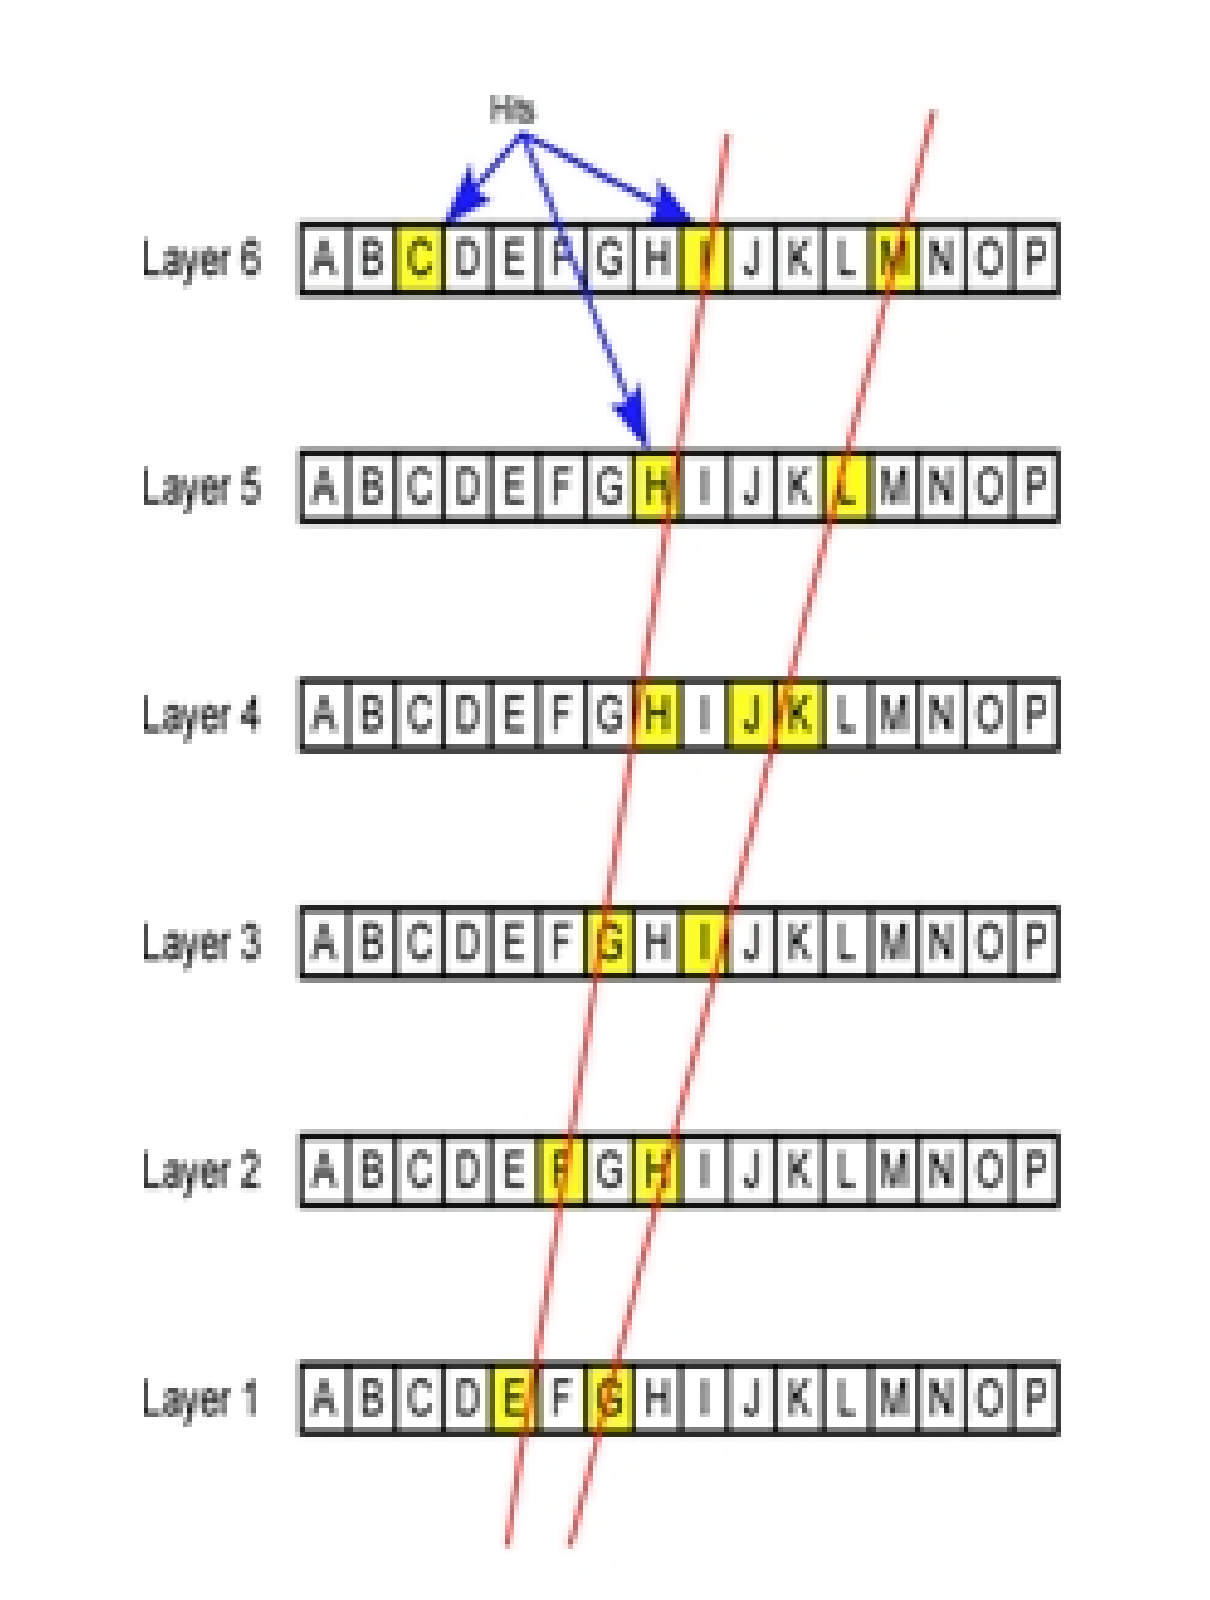
\includegraphics[width=0.4\columnwidth]{Plots/AM_pple2.eps}
\caption{Tracks in a tracking detector}
\label{fig:AM_principle_1}
\end{figure}

\noindent The Associative Memory (AM) architecture is based on Content Addressable Memory (CAM) cells~\cite{bib:Koh-87,bib:Pag-06} to efficiently identify track patterns (roads) at high speed using coarse-resolution 'hits' recorded in the tracking detector. A block diagram~\cite{bib:Rist-89} of the Associative Memory architecture is shown in Fig. 2 (for a case with four detector layers).  Each pattern (shown as a cell) is composed of four hit coordinates each of which is stored in the CAM word for a given layer, and only four patterns (cell 0 to 3) are shown in Fig.~\ref{fig:AM_principle_2}. 

\begin{figure}[ht!]
\centering
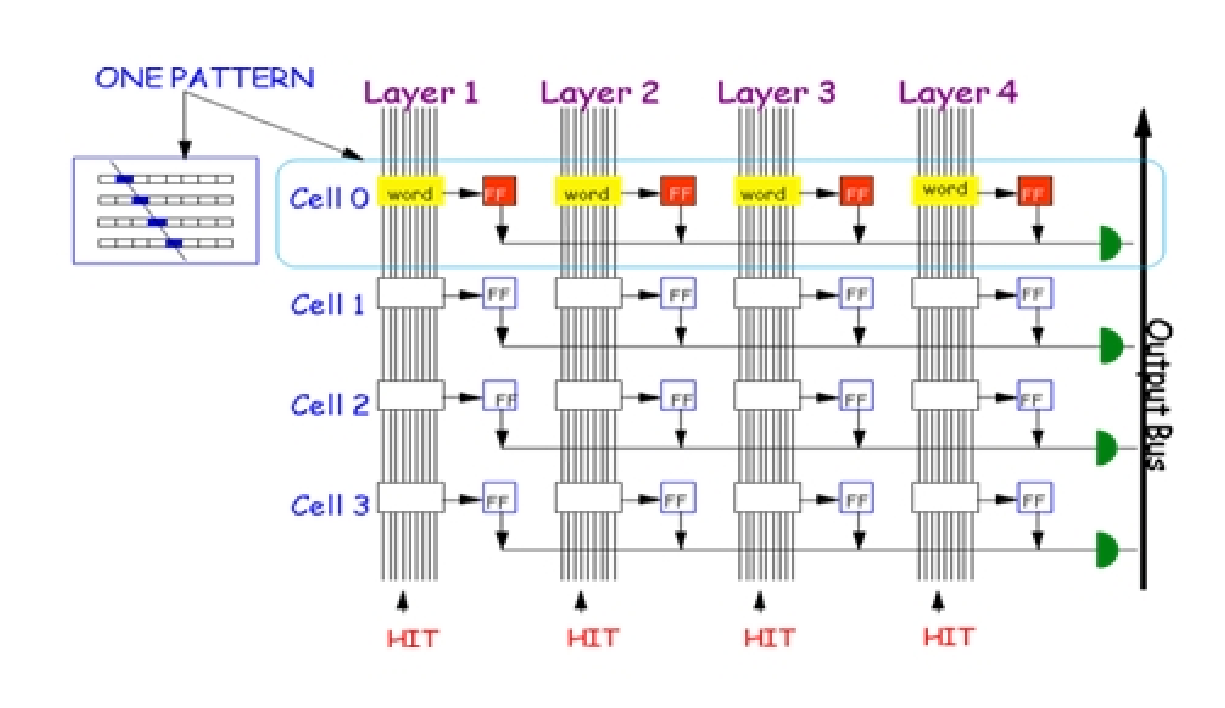
\includegraphics[width=0.9\columnwidth]{Plots/AM_pple.eps}
\caption{A block diagram on an associative memory chip. The CAM cells are shown as white (or yellow) boxes. The majority/glue logic is shown to the right as semi-circles.}
\label{fig:AM_principle_2}
\end{figure}

\noindent An incoming hit from a given detector layer is transmitted to the corresponding layer and the hit coordinate is compared against the stored words for all patterns in parallel for that layer. Any match to each incoming hit will be latched for that layer an
d for that pattern until reset (to rearm for next event). This process is repeated for all the incoming hits for each detector layer as the hits arrive one after the other. As soon as all hits from the same event are received, the hit matching stage is done and all latched matches for each pattern (or cell) will be fed into a majority logic stage where a fired road will be found if the number of matched layers reaches a programmable threshold. 
 

\noindent Associative Memory is sometimes called PRAM, Pattern Recognition Associative Memory. The AM method solves the combinatorial challenge inherent to the pattern recognition by exploiting massive parallelism of associative memories that can compare tracking detector hits to a set of pre-calculated patterns simultaneously. The found patterns or "fired roads" are then processed using fast FPGAs to perform track fitting with full detector resolution using all combinations of the "hits of interest" from the fired roads. Because each pattern or road is narrow enough, the usual helical fit can be replaced by a simple linear calculation. The track fitting stage for each matched pattern is much simplified and can be very fast~\cite{bib:Ann-09}.

\subsection{Trigger Tower, Sector, superstrip, and pattern banks}

\noindent We have described the concept of Trigger Tower in Section 2. Here we will describe the concept of sector, superstrip and pattern banks for the AM approach.

\noindent The pattern generation procedure starts by identifying first the sectors, which consists of one silicon module in each detector/logical layer. The list of sectors is determined with a training procedure that uses a large number of single muon (negative and positive) events, to cover all possible combinations of modules compatible with tracks coming from a region around the nominal beam spot position. The concept of sector is important because it is the region in which the linear track fit with one set of constants is performed (see later track fitting stage).

\noindent Each pattern is made of one superstrip per layer. A superstrip is a group of strips/pixels, and is therefore heavily constrained by the detector itself. Once the superstrip definition has been set, its position information is coded in a N-bits word: the superstrip address. It is important to realize that the AM-based pattern recognition is using these addresses, and is therefore independent from the detector geometry. As the addresses are transmitted to the AM independently for each layer, layer number doesn't have to be in the address word. 

\begin{figure}[ht!]
\centering
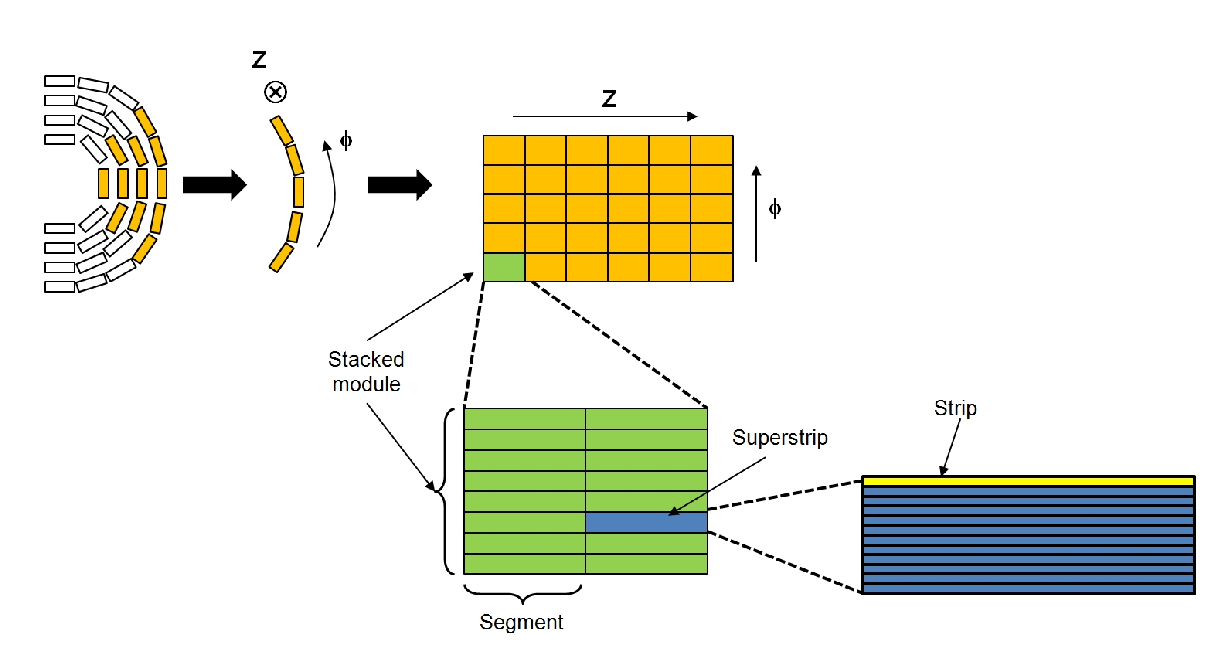
\includegraphics[width=0.8\columnwidth]{Plots/SStripDef.eps}
\caption{Geometric definition of a superstrip (barrel example).}
\label{fig:Det_to_SS}
\end{figure}
\begin{figure}[ht!]
\centering
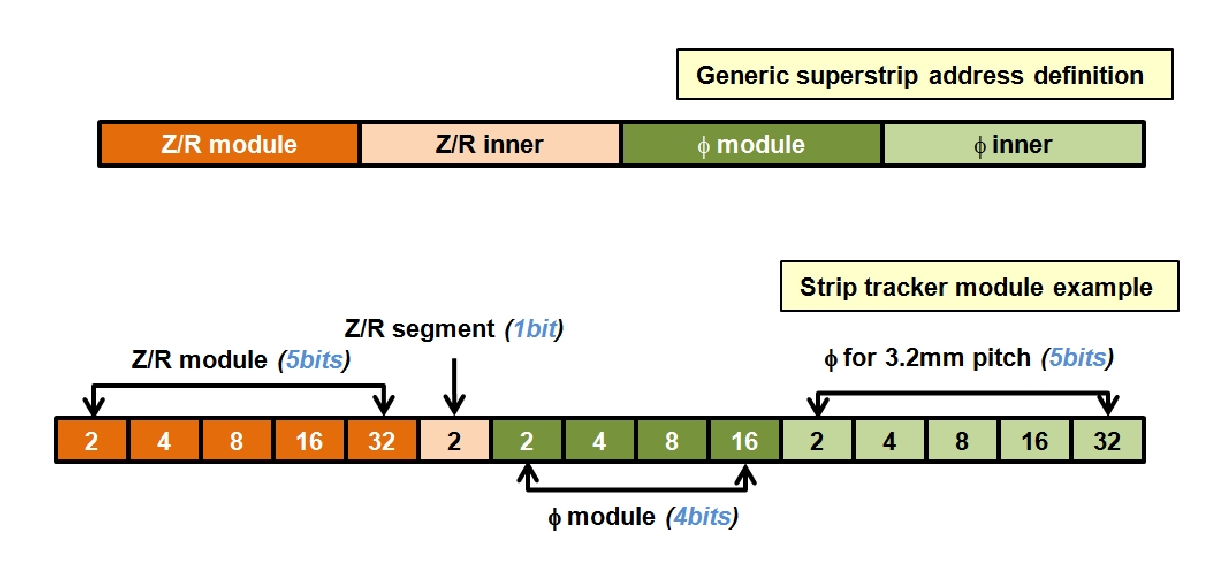
\includegraphics[width=0.6\columnwidth]{Plots/SSaddress.eps}
\caption{Address definition of a superstrip.}
\label{fig:SS_def}
\end{figure}

\noindent In order to understand the address definition, Fig.~\ref{fig:Det_to_SS} shows how a superstrip is defined in the barrel part of the tracker. Figure~\ref{fig:SS_def} shows the address definition of a superstrip. The number of bits necessary reflects the superstrip granularity and is constrained by the maximal word size acceptable by the AM chip (default is 15 bits). A first set of bits provides the module number along the corresponding coordinate: 5 bits for Z (one could have up to 24 modules in Z in one sector) and 4 for ? (up to 11 modules per sector in the outermost layer). Then, for each coordinates, a second series of bits provide the superstrip position within the module. Fig. 6 shows a tracker strip module (in green), divided into 2 segments in Z and 1024 strip in ?. Therefore in order to describe all the position, one would need only 1 bit for Z, and 10 bits for ?. In practice, a certain number of strips are grouped to form the superstrip, in our case 32, thus leading to 5 in the address. For the endcap the coding is the same, with z being replaced by r (equivalence is made between disks and layers, ladders and rings). 



\clearpage

%\section{Simulation tool development}

\subsection{The importance of simulation tools}

\noindent AM-based L1 tracking is a relatively complex task requiring a precise modelization before going to hardware implementation. This modelization is done via a dedicated simulation framework comprising:

\begin{itemize}
\item The model of the new tracker geometry implemented within the official CMS software chain (CMSSW)
\item The definition of the trigger tower
\item The definition and the production of the pattern banks for each trigger tower
\item The emulation of the AM-based pattern recognition within CMSSW
\item A set of track fitting procedures compatible with an FPGA implementation, coded within CMSSW
\end{itemize}

\noindent The following sections of this part are providing a description of the different steps necessary to setup this modelization. 

\subsection{Tracker geometry and trigger tower definition}

\noindent The geometry description and the trigger sector definition is provided by a standalone program: the TkLayout tool~\cite{bib:TkLayout}. For the geometry, this tool builds the xml files necessary to the CMSSW simulation stage. Then, using rates obtained from simulation and L1 tracking trigger requirements (in particular the minimal $p_T$ required for the tracks), the TkLayout tool can be used to optimize the trigger towers definitions. The goal here is to define the largest possible towers with a reasonable input data rate per layer, and to minimize the data sharing between towers. After performing this task, the TkLayout tool provides a simple text file containing, for each sector, a list of the tracker modules belonging to that sector. This file defines the structure of the track trigger system, and is hence is the basis of the L1 tracking stage.
  
\subsection{Pattern bank generation}

\noindent Bank generation is done via a dedicated standalone C++ program~\cite{bib:AMEmulator}. The main bank generation procedure is sketched on Fig.~\ref{fig:BkGen}. In order to produce a bank, two inputs are needed: a large simulated sample of single particle gun events (traditionally muons) covering the whole L1 track trigger acceptance requirements, and the TkLayout file providing the trigger towers definition.

\begin{figure}[ht!]
\centering
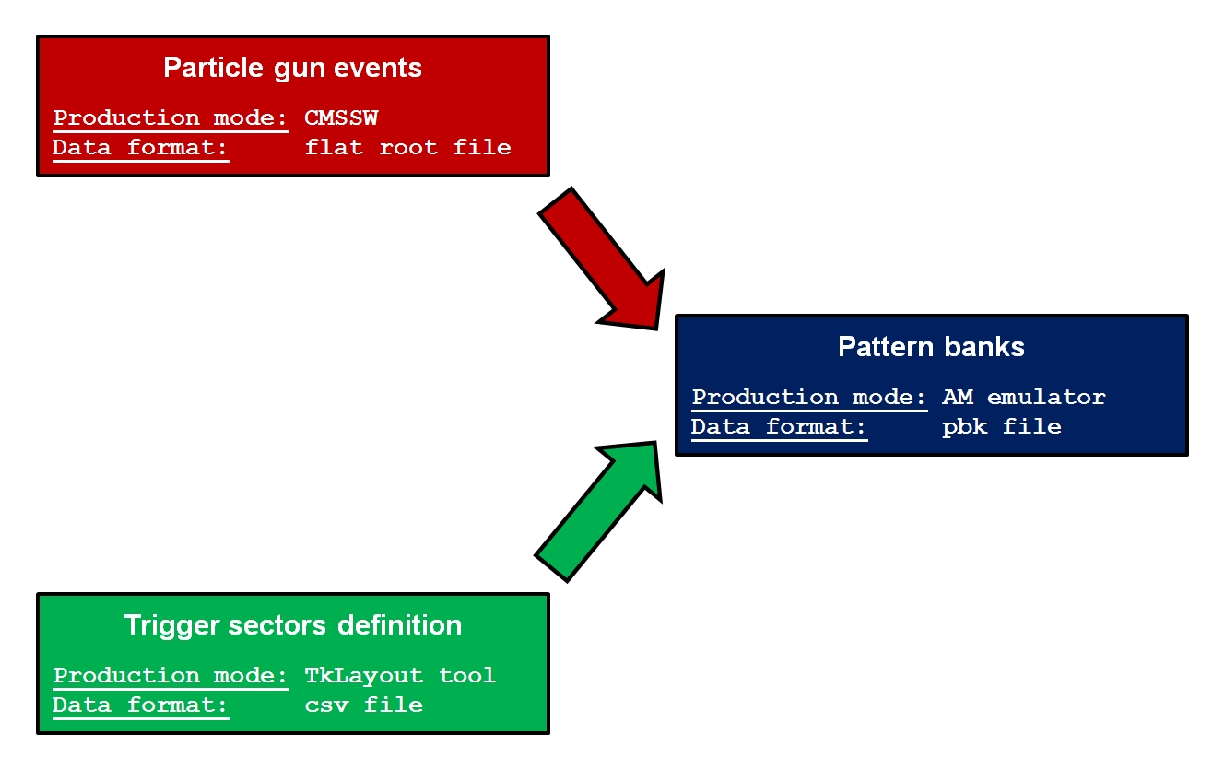
\includegraphics[width=0.6\columnwidth]{Plots/BankGen.eps}
\caption{Pattern bank generation principle}
\label{fig:BkGen}
\end{figure}

\noindent Based on these inputs, the code is able to produce a pattern bank for any trigger tower. Bank parameters can be set in the configuration file of the generation job. A complete description of the available option is provided in~\cite{bib:AMEmulator}.  

\noindent The bank generation algorithm, as it is implemented in the emulator, is summarized on Fig.~\ref{fig:BkGenDet}.

\begin{figure}[ht!]
\centering
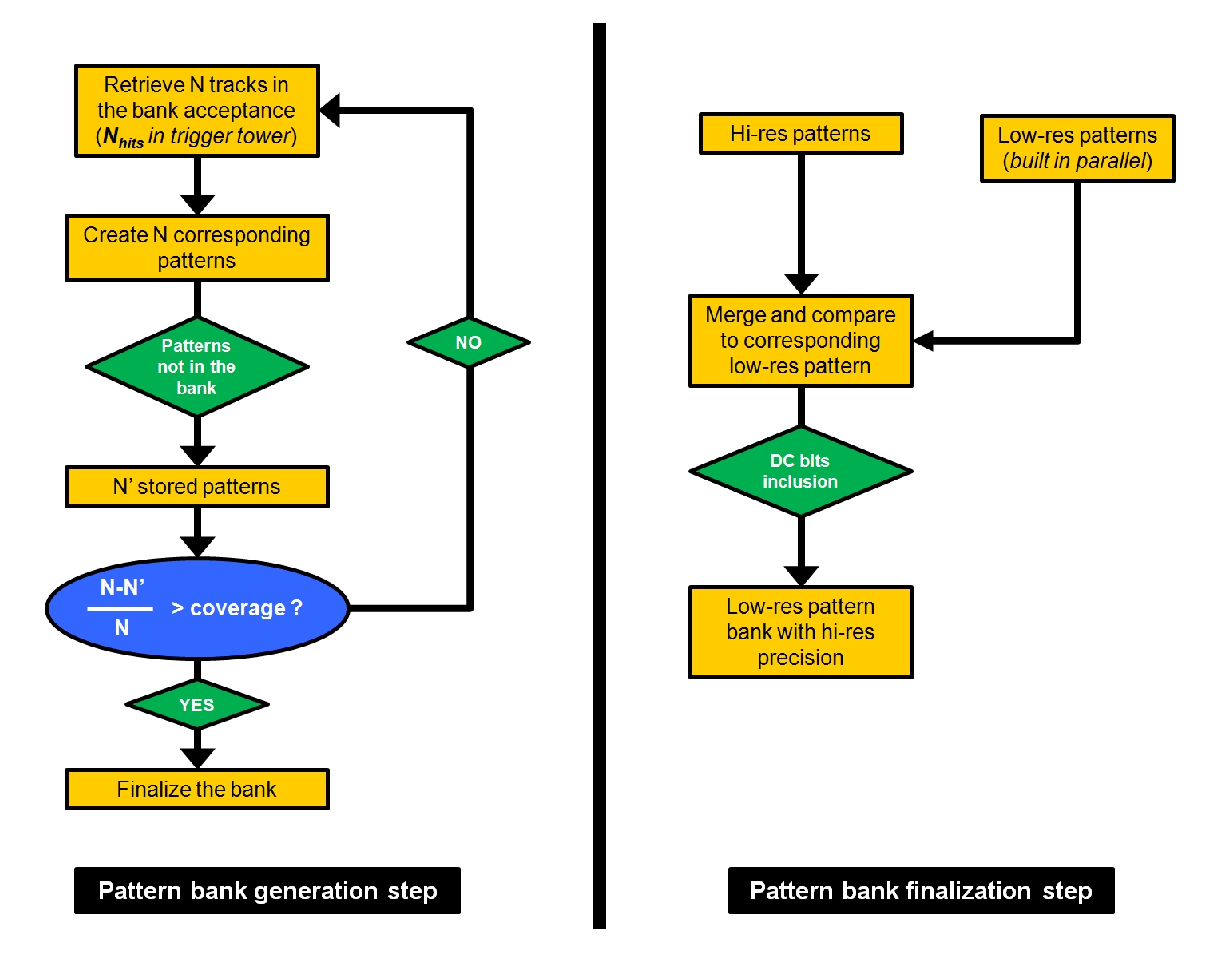
\includegraphics[width=0.6\columnwidth]{Plots/BankGenDetail.eps}
\caption{Pattern bank generation workflow: from track sample to pattern bank}
\label{fig:BkGenDet}
\end{figure}

\noindent This algorithm can be divided into two steps: bank production and bank finalization. As shown on the left diagram, the bank production is performed iteratively. An iteration starts by the collection of a set of $N$ tracks satisfying the pattern bank acceptance requirements in the input data sample (in our case $N=40000$). This acceptance requirement is defined by the parameter $N_{hits}$, which corresponds to the number of different layer/disks in which the particle has induced stubs in the trigger tower considered\footnote{This number should not be confused with the total number of stubs induced by the particle. If a track induces two stubs in a given layer (for example in an overlap area), these stubs will just count as one in $N_{hits}$.}.

\noindent A track can be used to produce a pattern only if its $N_{hits}$ value is equal to the pattern size set in the job configuration. Of course the pattern made from the track is stored in the bank only if not already in. Iteration ends when $N$ tracks have been collected. At this point, the proportion of tracks collected which were leading to an already stored pattern is computed. If this proportion, defined as the bank coverage, is larger than the coverage initially required, the iteration stage stops.

\noindent Once the required coverage has been reached, the bank is finalized. The procedure is described in the right part of Fig.~\ref{fig:BkGenDet}. At this point, it's not one, but two banks which have been built. Indeed, each new pattern is automatically linked to a low-resolution mother pattern. The resolution of this mother pattern is direclty related to the number of DC bits. The width of the low-res patterns is indeed $2^{N_{DC}}$ larger than the width of the high-res ones. For example, if one requires 2 DC bits, and built pattern with a superstrip size of 32 strips, the width of the low resolution patterns will be 128 strips. 

\noindent The low-res bank building follows the same procedure than the hi-res bank. But in addition, each low-res patterns is linked to a set of hi-res patterns. Before storing the low-res pattern in the banks, hi-res patterns belonging to it are merged. The merging result is then compared to the low-res pattern, and the hi-res granularity is kept whenever possible. On the other hand, if all the super-strips are used in a given layer, corresponding DC bits are applied.

\noindent Using this procedure provides the possibility to get high-resolution precision for the price of a low resolution bank. 


\subsection{Pattern recognition}

\subsubsection{Software principle}

\noindent The pattern recognition is done using the same code than the bank generation. This code has been interfaced with the CMS software framework (CMSSW). It uses the official CMSSW stubs and stores the patterns as official CMSSW track seeds. For debugging purposes, the pattern recognition code can also work standalone, starting from plain rootuple containing the stubs of a given event. 

\noindent The code is working for a given sector. The complete pattern recognition of a given event therefore requires to run in parallel jobs for every trigger tower. The data merging is performed afterwards, so that the final output contains for each event the pattern recognition outcome for all the towers. 


\subsubsection{Estimation of the pattern recognition efficiencies and fake rates}

\noindent The basis of the pattern recognitionefficiency is the number $N$ of matchable tracks. This number is depending on the size of the patterns stored. For patterns made of 6 superstrips, if a missing hit is accepted, any track crossing at least 5 layers in the tower will matchable. 

\noindent The number of layers/disks crossed by the particle within one tower is therefore an important parameter. From now own, it will be mentioned in all the notations. For example, $N_{5}$ corresponds to the number of tracks crossing at least 5 layers/disks in one of the trigger tower.

\noindent Starting from there, the efficiency for a given threshold could be defined as the number of tracks matched in a pattern divided by the total number of tracks: 
\begin{equation}
\epsilon_i = \frac{N^{matched}_i}{N_i}
\end{equation} 

\noindent Then, we define the fake rate as the proportion of patterns which are not containing a good track. 
\begin{equation}
\rho_i = \frac{N^{bad patterns}_{i}}{N^{patterns}_{i}}
\end{equation} 

\noindent This fake rate definition doesn't account for the duplicated patterns. This value is measured by the redundancy,which corresponds to the average number of patterns activated by each good track. The ideal pattern bank for a given threshold $i$ is the one for which $\epsilon_i = 1$ and $\rho_i = 0$.

\noindent Such a bank exists, this is the one for which each possible track in the detector corresponds to one pattern. However, the size of such bank will be prohibitive. On the other side, one could imagine the simplest bank with 1 single pattern defined by the whole detector. Such a bank will have $\epsilon=1$, $\rho = 0$ and $r = 1$, but $\epsilon_{hits}$ will be close to 0. Such a solution would be highly inefficient, as TF would be impossible to process. Therefore the optimal solution lies in between, and one realizes that a parameter will be very important: the size of the patterns. The patterns will have to be sufficiently small in order to get a reasonable $\epsilon_{hits}$, but also sufficiently large in order get a reasonable pattern bank size. 

\noindent Finding the optimal bank is a complex exercise which will be done for the TDR, and hence is beyond the scope of this preparatory note. In this document we present preliminary results obtained using a simple set of pattern banks, which where produced using a large sample of particle gun $\mu^{\pm}$ produced within the following phase space:
\begin{itemize}
\item $0 < \eta_0 < 2.2$.
\item $1.95GeV/c < p_{T_0} < 100GeV/c$, generated randomly in $1/p_T$.
\item $-15cm < z_0 < 15cm$.
 \item $-1mm < d_0 < 1mm$.
\end{itemize}  

\noindent In order to cover correctly the whole $pT$ phase space the sample was divided into three $pT$ ranges: 1.95 to 5 GeV/c, 5 to 20, and 20 to 100. Patterns were made from 32 to 256 strips-wide superstrips (we generate 32 strips banks and used 3 DC bits) in order to get banks of ~1M patterns for each trigger tower. The total number of patterns necessary to cover all the tracker in this configuration is 64~Millions. 

\noindent The following table summarizes the overall efficiencies and fake rates obtained for simple single particles with $p_T>2GeV/c$ using the banks described previously, for $N_{hits}=5$.

\begin{table}[ht!]
\centering
\begin{tabular}{|c|c|c|c|}
  \hline
  Particle type & Muons & Pions & Electrons \\ \hline
  Efficiency ($\epsilon_5$, in \%) &  &  &  \\ \hline
  Fake rate ($\rho_5$, in \%) &  &  &  \\\hline
\end{tabular}
\caption{Stub repartition in the tracker, measured with PU=200 events.}
\label{tad:dev}
\end{table}

\noindent Figures~\ref{fig:PRMU} and {fig:PRELE} shows a summary of the pattern recognition outcome for muons and electrons respectively. The broader turn-on for electrons is mainly due to multiple scattering.

\begin{figure}[ht!]
\begin{minipage}[t]{7.5cm}
\centering
%\includegraphics[width=0.75\textwidth]{Plots/Muon.eps}
\caption{Pattern recognition efficiency for single muons}
\label{fig:PRMU}
\end{minipage}
\hfill
\begin{minipage}[t]{7.5cm}
\centering
%\includegraphics[width=0.75\textwidth]{Plots/AdapSec.eps}
\caption{Pattern recognition efficiency for single electrons}
\label{fig:PRELE}
\end{minipage}
\end{figure} 

\noindent In order to evaluate the fake rate, two types of events were used. Both were overlaid with an average of 140 minimum bias events. In the first set, a single muon was added to minbias contents, whereas in the other sample, a four tops final state was added. This last sample could be considered as a worst case scenario for tracker occupancy, and is therefore particularly useful for studying the maximum rates per modules.   

\noindent The pattern recognition efficiency was also tested, as shown on Fig.~\ref{fig:PR_4tops} for the 4 tops events. As expected, the efficiency is robust against pileup. If a pattern is matched, it will always match independently from the stubs you add around it. What will change is the fake proportion. The fake rates, for both samples are summarized in the following table:

\begin{table}[ht!]
\centering
\begin{tabular}{|c|c|c|c|}
  \hline
  Particle type & Muons & Pions & Electrons \\ \hline
  Efficiency ($\epsilon_5$, in \%) &  &  &  \\ \hline
  Fake rate ($\rho_5$, in \%) &  &  &  \\\hline
\end{tabular}
\caption{}
\label{tad:dev}
\end{table}

\subsubsection{Bank efficiency definition}


\subsection{Further developments and improvements}


\clearpage

%\section{Track Trigger Performance Requirements}

\subsection{Tracking performance}

\subsection{Performance on trigger objects}

\subsection{Selected physics cases}

\clearpage


\end{document}
